%% Love at First Sprite: the Yi Town paper.
%% Build: pdflatex love-at-first-sprite && bibtex love-at-first-sprite && pdflatex love-at-first-sprite && pdflatex love-at-first-sprite
%% (TinyTeX: export PATH="$HOME/Library/TinyTeX/bin/universal-darwin:$PATH")
\documentclass[sigconf,nonacm]{acmart}

\usepackage{CJKutf8}
\usepackage{tikz}
\usetikzlibrary{arrows.meta,positioning,fit,calc,shapes.geometric}
\usepackage{subcaption}
\usepackage{booktabs}
\usepackage{multirow}
\usepackage{enumitem}
\usepackage{balance}

% Chinese in a Latin paper: Arphic Song for running text, Arphic Kai for quoted verse.
\pdfmapfile{+gbsnu.map}
\pdfmapfile{+gkaiu.map}
\newcommand{\zh}[1]{\begin{CJK*}{UTF8}{gbsn}#1\end{CJK*}}
\newcommand{\kai}[1]{\begin{CJK*}{UTF8}{gkai}#1\end{CJK*}}

% The town's palette, used in the diagrams.
\definecolor{navy}{HTML}{0B2036}
\definecolor{gold}{HTML}{D3A557}
\definecolor{cream}{HTML}{F6EFE2}
\definecolor{rose}{HTML}{C74B5F}
\definecolor{meadow}{HTML}{5F9E5A}
\definecolor{sky}{HTML}{3F7FB3}

\newcommand{\yt}{Yi Town}
\newcommand{\code}[1]{\texttt{\small #1}}
\newcommand{\dc}[1]{\textsc{D#1}}

\settopmatter{printacmref=false, printccs=true, printfolios=true}
\renewcommand\footnotetextcopyrightpermission[1]{}
\setcopyright{none}

\begin{document}

\title{Love at First Sprite}
\subtitle{A Pixel Town for Two, Thirteen Hours and One Ocean Apart}

\author{Jingyi Chen}
\affiliation{\institution{Yi Town}\country{}}

\author{Yifan Yang}
\authornote{Corresponding author.}
\affiliation{\institution{Yi Town}\country{}}
\email{yyf990925@gmail.com}

\renewcommand{\shortauthors}{J. Chen and Y. Yang}

\begin{abstract}
Two people met on 20 September 2026 and have since lived thirteen hours and one Pacific Ocean
apart, one in Shenzhen, China, the other in College Station, Texas. This paper reports the
design and implementation of \yt{}, a bilingual, browser-only game made by this couple for
themselves, first as a birthday gift and then as a shared artefact that keeps growing. Each
player walks a pixel avatar through a small town whose nine houses are levels, and each level
turns one shared memory into a game mechanic: a vow spoken aloud and recognised in the browser,
street views to be named on a map of six places, a tattoo handwritten on a drawn arm, a timeline
to put back in order, Gomoku endgames whose answers trace a heart, songs named from a passage,
the stars of two birth signs joined by hand, missing characters restored to classical Chinese love
poems, and a procedurally modelled ring tried on through hand tracking. A birthday prologue and a
wedding finale play as pixel cutscenes. Using research through design and autobiographical
design, we state six design commitments (memory as mechanics, earned access, intimacy without a
server, parity between the two languages, art drawn in code, and secrecy as narrative tension)
and show how the system realises each of them. Progress is modelled as a grow-only set, so
merging two devices' progress needs no server. It travels between phones as a code of at most
four characters guarded by an ISO~7064 MOD~37,36 check character. The sky follows each player's
own clock, and a unit test keeps the final surprise out of every string shown before it. The
system comprises about 8{,}400 lines of strict TypeScript and 153 unit tests and was built in 109
commits over five days. We reflect on what designing for an audience of exactly one other person
reveals about privacy, asynchrony and ceremony in intimate computing.
\end{abstract}

\begin{CCSXML}
<ccs2012>
<concept><concept_id>10003120.10003121.10003129</concept_id>
<concept_desc>Human-centered computing~Interactive systems and tools</concept_desc>
<concept_significance>500</concept_significance></concept>
<concept><concept_id>10003120.10003130.10003131</concept_id>
<concept_desc>Human-centered computing~Collaborative and social computing theory, concepts and paradigms</concept_desc>
<concept_significance>300</concept_significance></concept>
<concept><concept_id>10010405.10010476.10011187.10011190</concept_id>
<concept_desc>Applied computing~Computer games</concept_desc>
<concept_significance>300</concept_significance></concept>
</ccs2012>
\end{CCSXML}
\ccsdesc[500]{Human-centered computing~Interactive systems and tools}
\ccsdesc[300]{Human-centered computing~Collaborative and social computing theory, concepts and paradigms}
\ccsdesc[300]{Applied computing~Computer games}

\keywords{intimate computing, long-distance relationships, autobiographical design, research through design,
games for two, local-first software, bilingual interfaces, pixel art, ceremony, surprise}

\begin{teaserfigure}
  \centering
  \begin{subfigure}[b]{0.25\textwidth}
    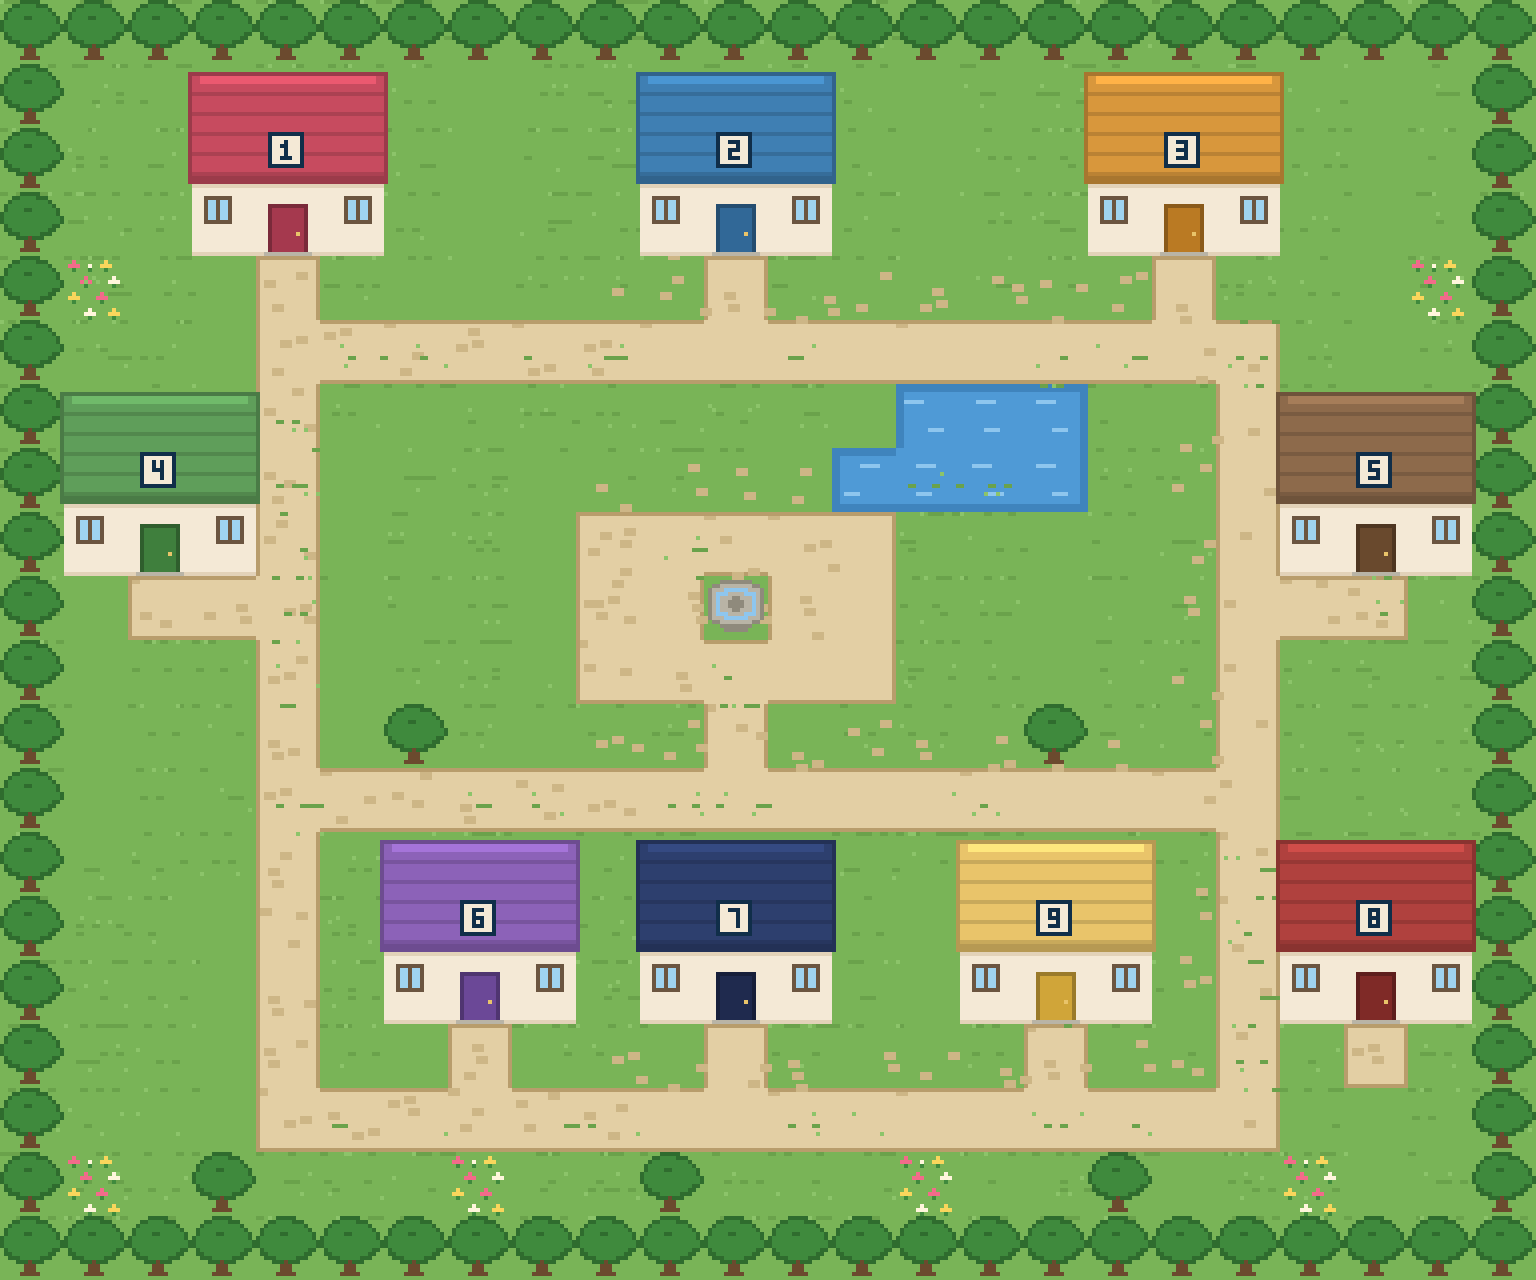
\includegraphics[width=\linewidth]{figures/art-town.png}
    \caption{The whole town, drawn in code}\label{fig:teaser-map}
  \end{subfigure}\hfill
  \begin{subfigure}[b]{0.235\textwidth}
    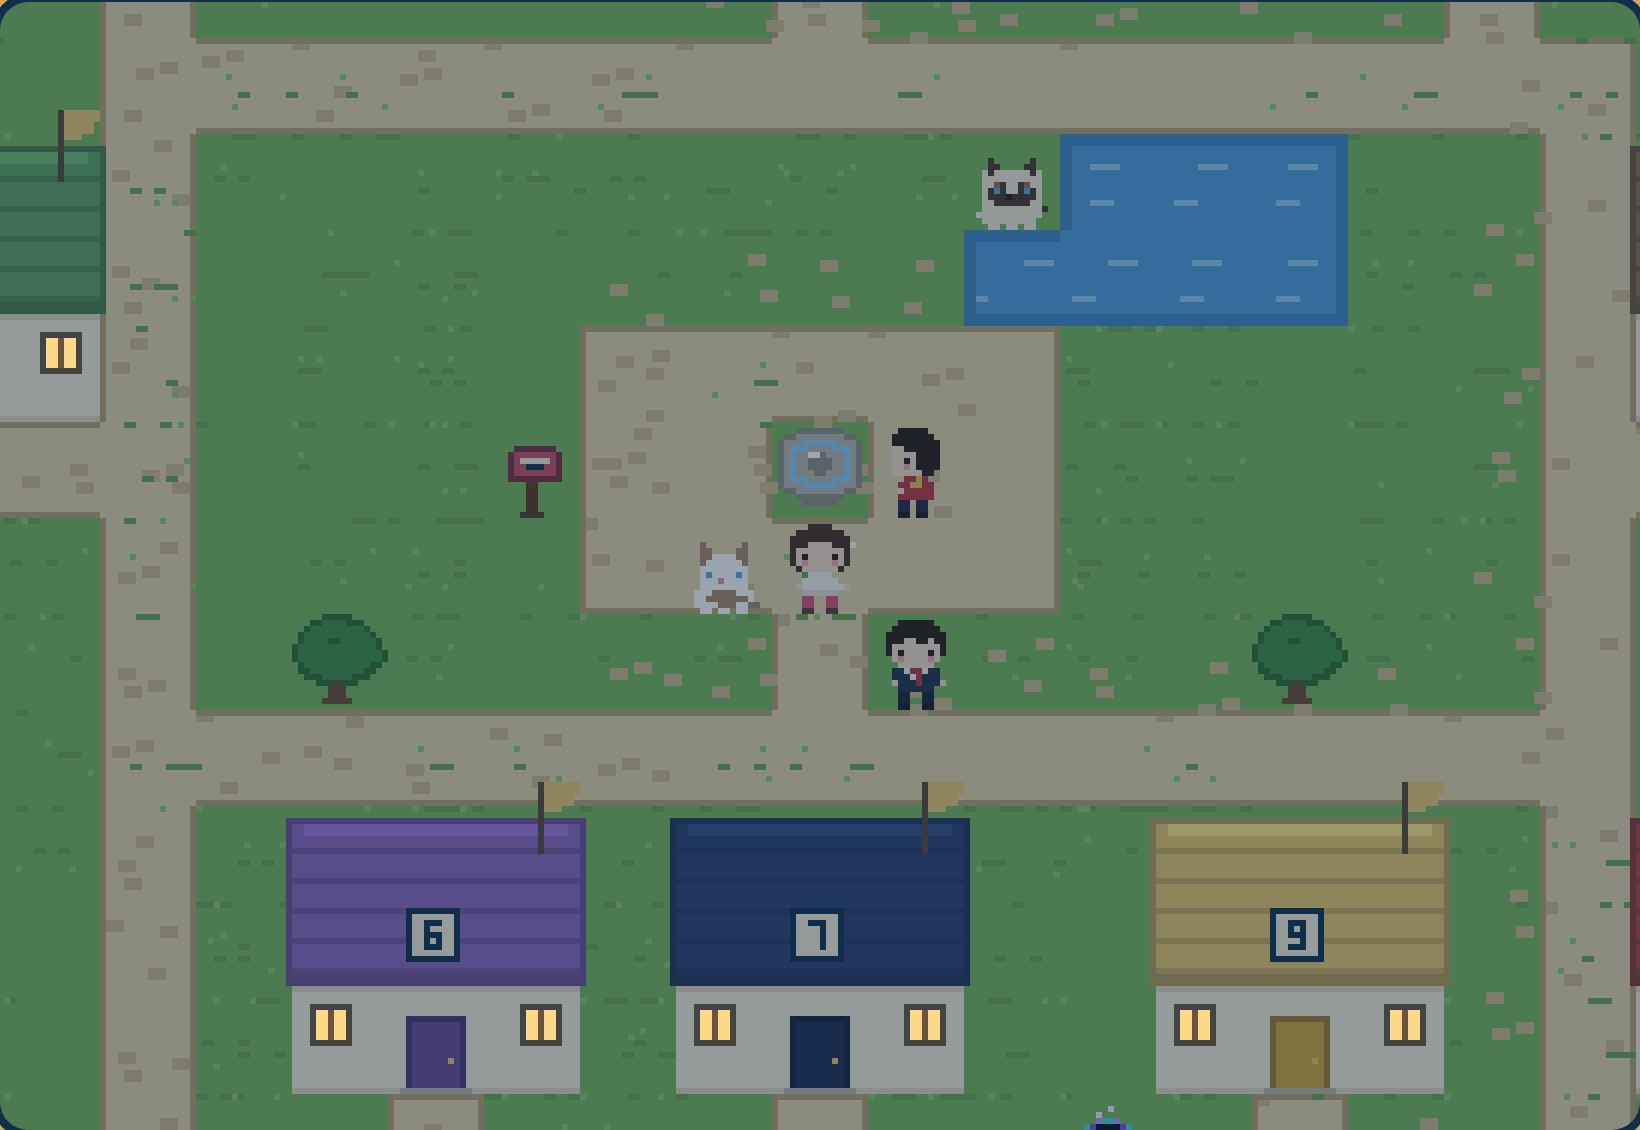
\includegraphics[width=\linewidth]{figures/town-done-canvas.jpg}\\[2pt]
    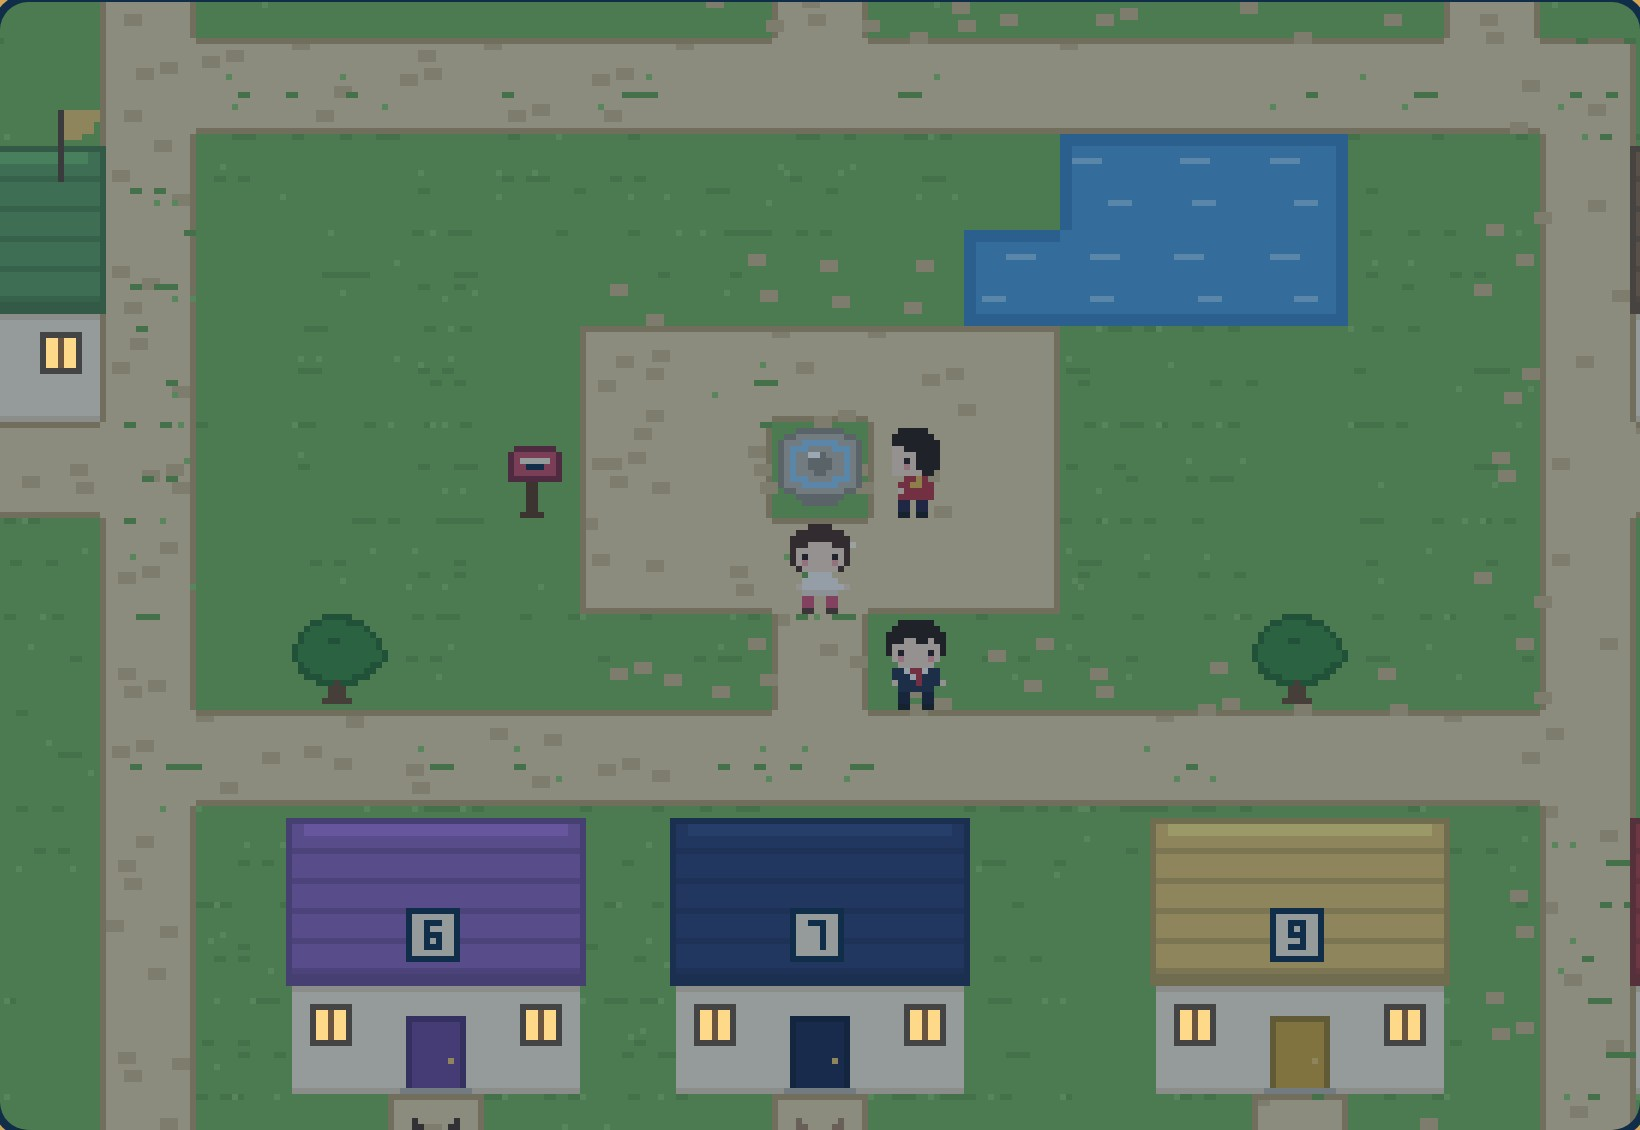
\includegraphics[width=\linewidth]{figures/town-canvas.jpg}
    \caption{The square: guide, partner, cats}\label{fig:teaser-square}
  \end{subfigure}\hfill
  \begin{subfigure}[b]{0.245\textwidth}
    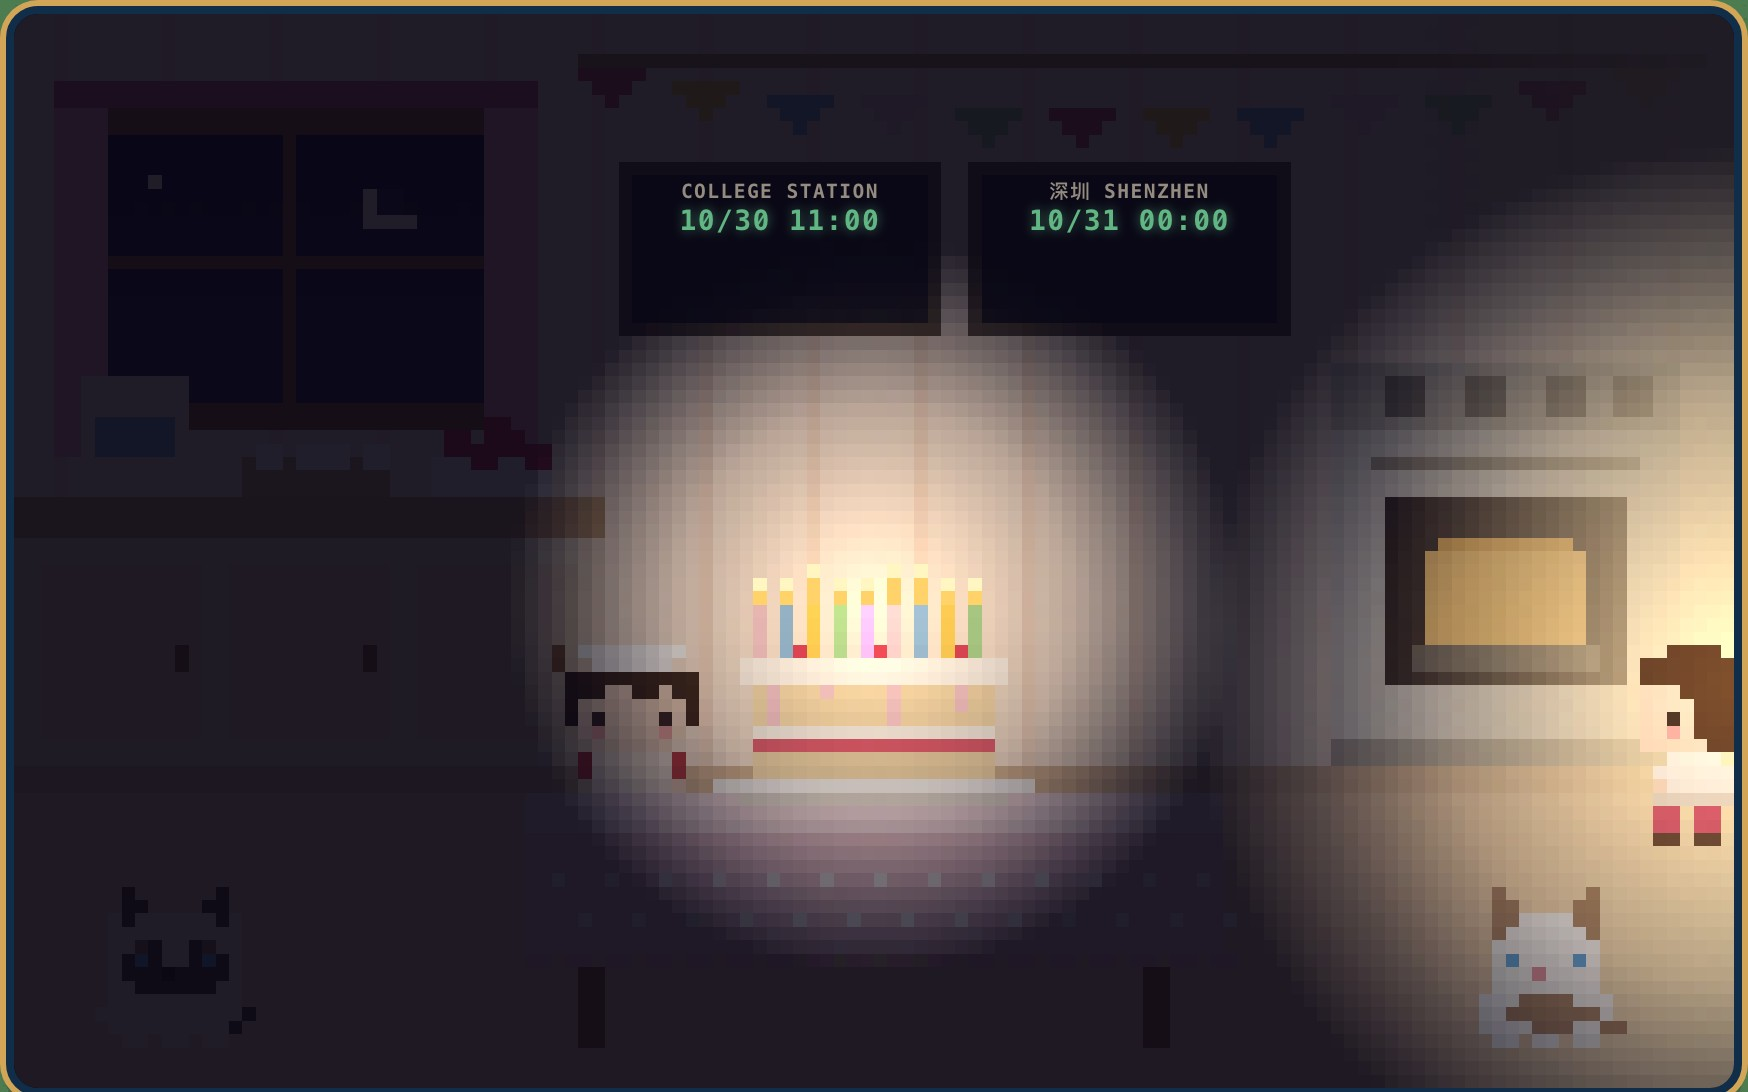
\includegraphics[width=\linewidth]{figures/bday-34.jpg}\\[2pt]
    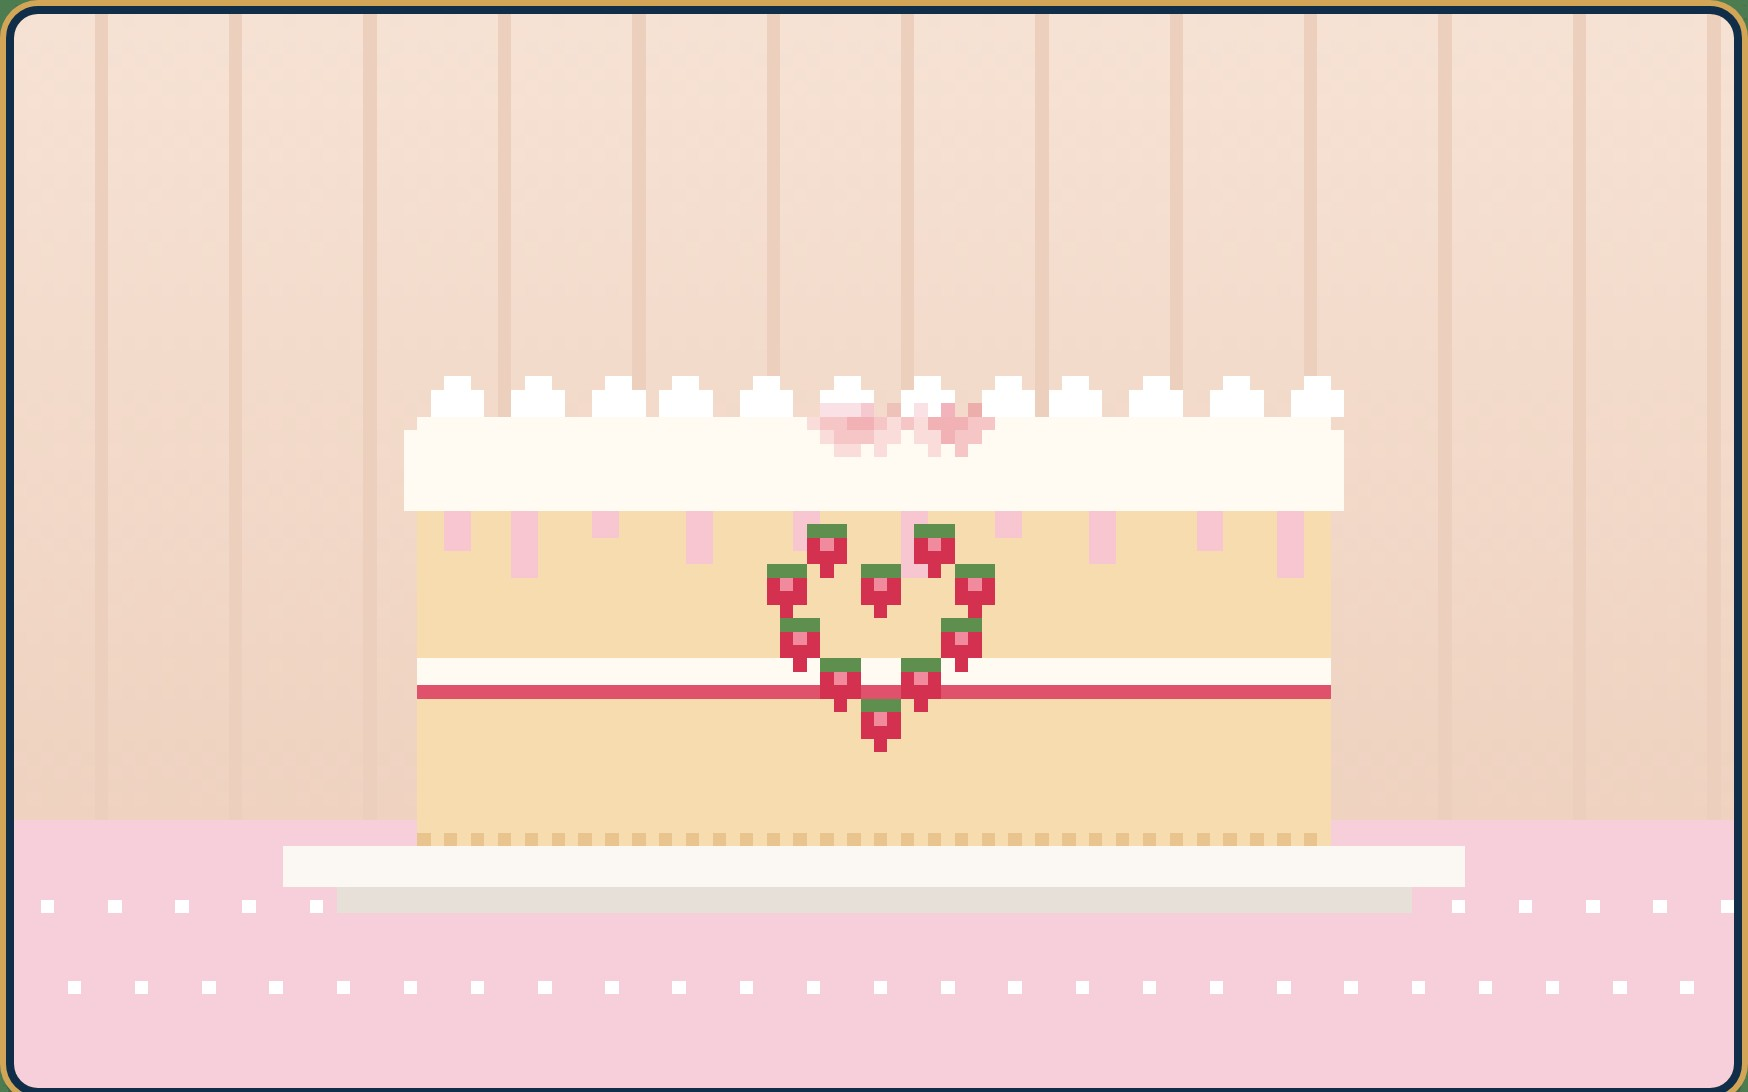
\includegraphics[width=\linewidth]{figures/bday-24.jpg}
    \caption{Prologue: the birthday cake}\label{fig:teaser-bday}
  \end{subfigure}\hfill
  \begin{subfigure}[b]{0.245\textwidth}
    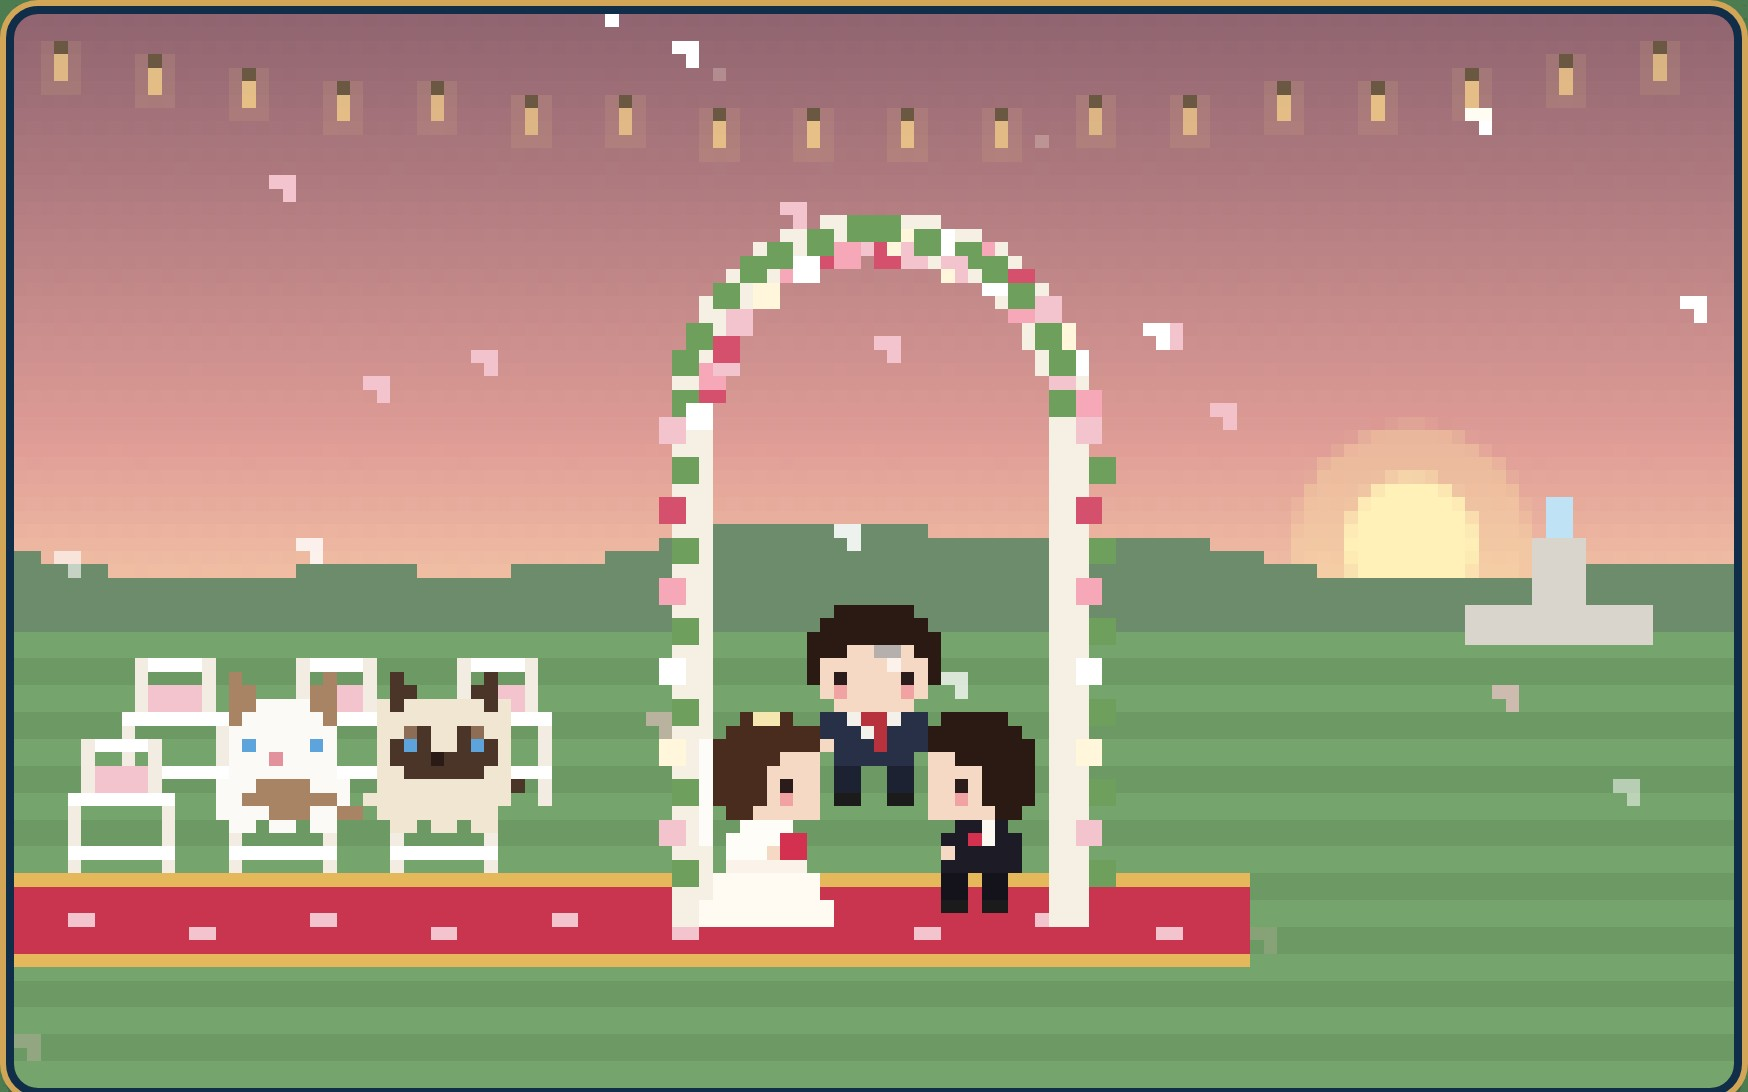
\includegraphics[width=\linewidth]{figures/wed-13.jpg}\\[2pt]
    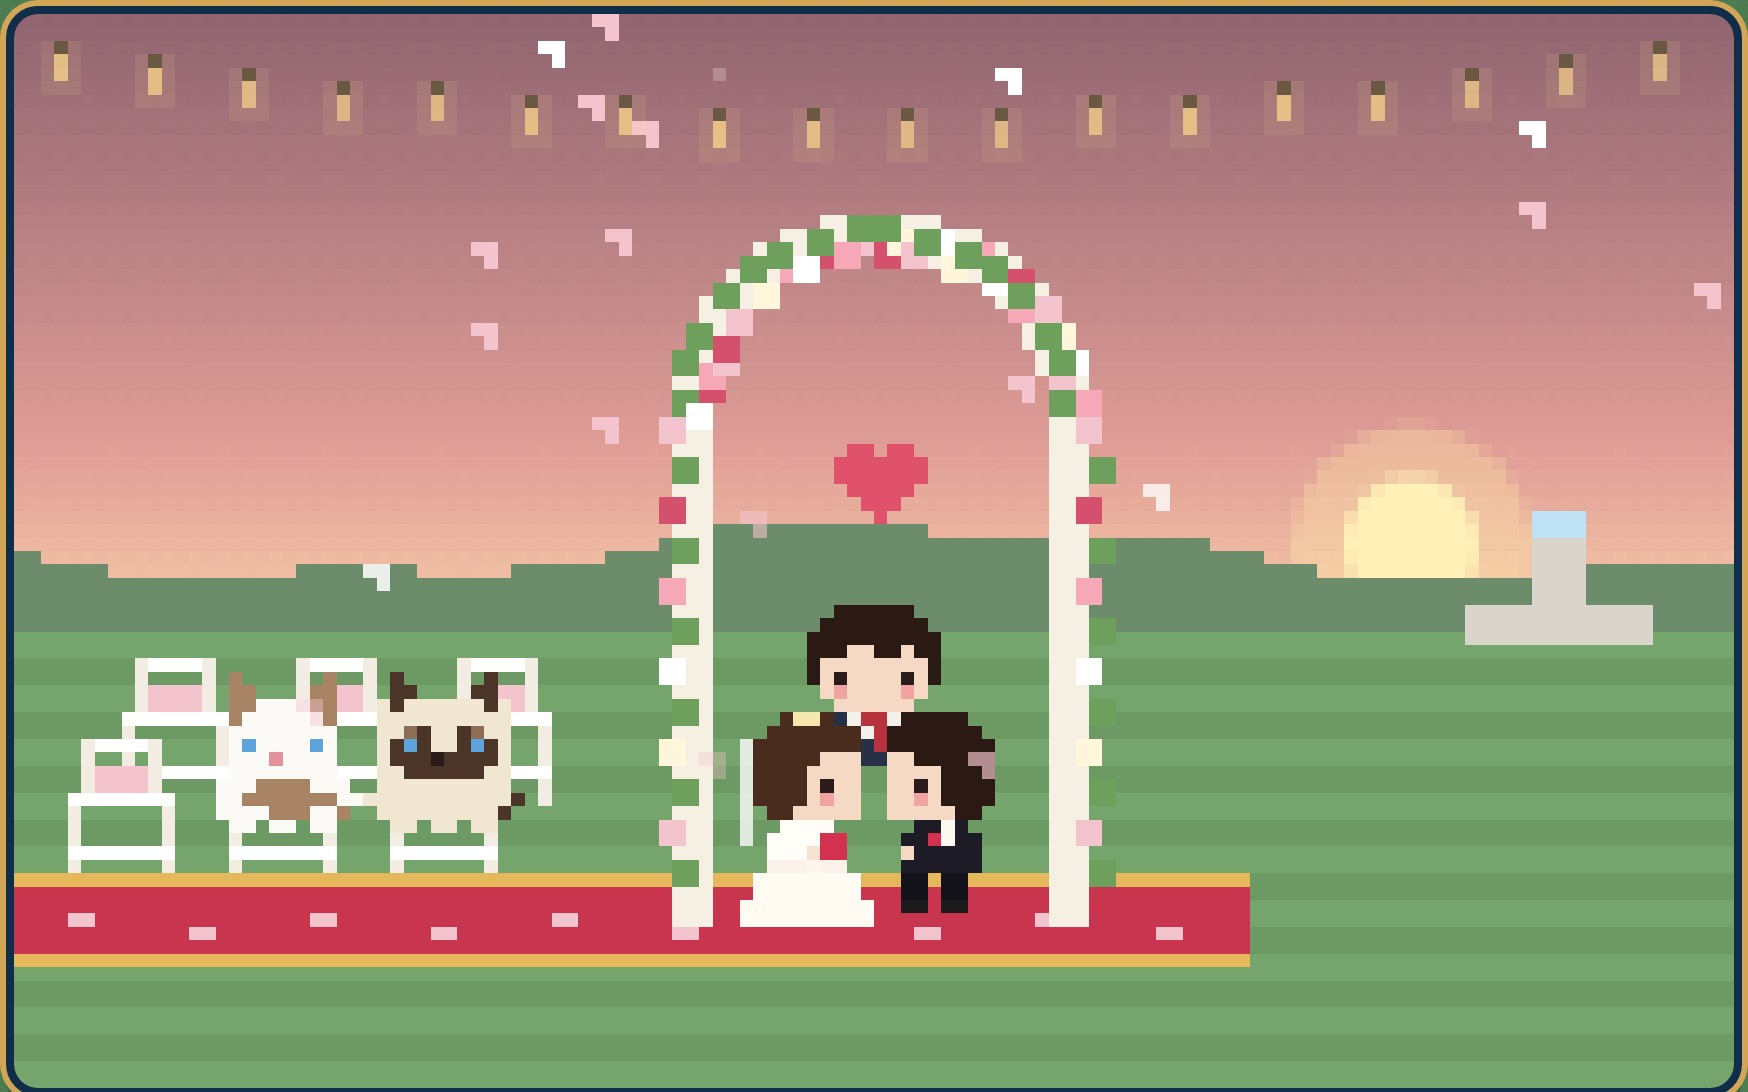
\includegraphics[width=\linewidth]{figures/wed-27.jpg}
    \caption{Finale: the wedding}\label{fig:teaser-wed}
  \end{subfigure}
  \caption{\yt{} at a glance. (a) The town map: a $24\times20$ grid of $16$-pixel tiles with nine
  numbered houses, one per level, painted entirely by code. (b) The fountain square in play, top
  after every level is cleared (gold flags, a cat sunbathing by the pond) and bottom halfway
  through; the player meets the partner, the guide Rayford and the cats. (c) The birthday
  prologue: nine candles in the dark at Shenzhen midnight, and ten strawberries set in a heart.
  (d) The wedding in the fountain garden, officiated by Rayford with the two cats as guests.}
  \Description{Four panels: a full pixel-art town map with nine coloured houses around a fountain;
  two close-ups of the square with small characters; two frames of a pixel kitchen with a lit
  birthday cake; two frames of a pixel wedding under a flower arch at sunset.}
  \label{fig:teaser}
\end{teaserfigure}

\maketitle

%% ===================================================================================
\section{Introduction}

Jingyi and Yifan met on 20 September 2026. From the first day they have lived on opposite
sides of the Pacific: Jingyi in Shenzhen, Guangdong, where she works in product management, and
Yifan in College Station, Texas, where he is a doctoral student. Between their
clocks lie thirteen hours, so that one of them is always walking home in the dark while the other
is starting a morning. Their next meeting is fixed by a plane ticket Yifan drew by hand on their
first video call (flight \emph{CYF925}, Shenzhen to New York, 5 February 2027, gate
\emph{LOVE910}, seat \emph{99A}).

Long-distance couples are not rare, and their communication is often more intimate, not less,
than that of couples who live together~\cite{jiang2013absence,stafford2005maintaining}. Human-computer
interaction (HCI) has long designed for such couples, from devices that pass a squeeze or a hug
across a distance~\cite{brave1997intouch,mueller2005hug,strong1996feather} to systems that share
the empty moments of a day~\cite{lottridge2009sharing,tsujita2008syncdecor} or one bit of
``I~am thinking of you''~\cite{kaye2006clicked}. These systems are built by researchers for couples
whom the researchers then study. The artefact in this paper reverses that relation. \yt{} was
built by one member of a couple, for the other and for himself, out of material that only the two
of them hold: the date they met, the songs they share, the photos, a first game played on a Zoom
whiteboard, the stars of their two birth signs.

\yt{} is a web game for exactly two players (Figure~\ref{fig:teaser}). After a question that
only the two can answer, a player picks who they are and walks a twelve-by-sixteen-pixel version
of themselves through a small town. The partner waits by the fountain. Each of the nine houses is
a level made from something that happened to the couple; a cleared house flies a gold flag, and the
two cats of the household, Coffee and Duoduo, sit at the next locked doors. The first time a player
arrives, a cutscene shows Yifan baking a birthday cake against the Shenzhen-midnight clock. When
both players have reached the last house, a letter opens, and after it a wedding.

This paper makes four contributions.
\begin{enumerate}[leftmargin=*,itemsep=1pt,topsep=2pt]
  \item A \textbf{design case} of an intimate game built autobiographically, for an audience of
  one other person, documented through its design log of 109 commits and 28 versions
  (Sections~\ref{sec:method} and~\ref{sec:experience}).
  \item Six \textbf{design commitments} for intimate play across distance, each traced to concrete
  mechanisms (Table~\ref{tab:commitments}).
  \item A \textbf{serverless architecture} for two-person progress: progress as a grow-only set
  whose merge is a union, carried between phones as a short checksummed code, with a sky that
  follows each player's local time and a test that guards the final surprise (Section~\ref{sec:system}).
  \item A \textbf{reflection} on privacy, asynchrony, bilingualism and ceremony when the designer,
  the player and the subject of the design are the same two people (Section~\ref{sec:discussion}).
\end{enumerate}

%% ===================================================================================
\section{Related Work}

\subsection{Mediating intimacy at a distance}
Vetere et al.\ studied how couples and families express intimacy and argued that technologies for
strong ties should support the expressive, the physical and the playful, not only the
informational~\cite{vetere2005mediating}. Hassenzahl et al.\ reviewed 143 intimacy-mediating
artefacts and grouped them into six strategies: awareness, expressivity, physicalness, gift
giving, joint action and memories~\cite{hassenzahl2012love}. Most systems they reviewed are
minimal channels: a lamp that lights when the partner touches theirs, a single button
whose meaning the couple negotiates~\cite{kaye2006clicked}. Neustaedter and Greenberg showed
that long-distance couples keep video calls open for hours to share ``being together'' rather
than to talk~\cite{neustaedter2012intimacy}; CoupleVIBE conveyed a partner's location by
vibration~\cite{bales2011couplevibe}; SyncDecor linked everyday appliances in two
homes~\cite{tsujita2008syncdecor}. \yt{} sits in Hassenzahl's \emph{memories} and \emph{gift giving}
strategies, but differs in scale and authorship: it is not a minimal channel but a whole world,
and its content is the couple's own history rather than a live signal.

\subsection{Autobiographical and first-person design}
Neustaedter and Sengers defined autobiographical design as design research drawing on genuine
use by the people who built the system~\cite{neustaedter2012autobiographical}, and Desjardins
and Ball documented its tensions, including the blurred line between designer and
participant, and the intimacy of the data involved~\cite{desjardins2018tensions}. First-person
methods, ``a sample of one''~\cite{lucero2019sample}, accept that what is learned is situated and
deep rather than general. Research through design treats the artefact itself as a carrier of
knowledge~\cite{zimmerman2007rtd,gaver2012expect}. \yt{} is autobiographical twice over: it is built
by one of its two users, and it is built \emph{out of} the two users' lives.

\subsection{Play, ritual and games for two}
Huizinga described play as a ``magic circle'' set apart from ordinary life~\cite{huizinga1955homo};
Salen and Zimmerman made the circle a design tool~\cite{salen2004rules}; Juul showed that games
are half real rules and half fiction~\cite{juul2005halfreal}. Sicart argued that play
appropriates the world and its objects~\cite{sicart2014play}, and Isbister showed how games build
connection between players through shared action~\cite{isbister2016games}. Ludic design in HCI
values curiosity and ambiguity over task efficiency~\cite{gaver2004drift,gaver2003ambiguity}, and
slow technology designs for reflection rather than throughput~\cite{hallnas2001slow,odom2012technology}.
Aron et al.'s procedure for generating closeness through escalating mutual
disclosure~\cite{aron1997closeness} is, in a sense, a level structure. \yt{} takes the game form
literally: locks, levels, a guide, a prologue and a finale, and play that follows the order of
a relationship that is still being lived.

\subsection{Local-first and serverless software}
Kleppmann et al.\ argued for local-first software that keeps the primary copy of data on the
user's device and works offline~\cite{kleppmann2019localfirst}. Conflict-free replicated data types
(CRDTs) guarantee convergence without coordination; the simplest, the grow-only set, merges by
union~\cite{shapiro2011crdt}. In intimate computing, keeping data on the device is as much a
matter of feeling as of security: photos, voice notes and letters between two people should not
live on a third party's server. \yt{} applies the grow-only set to a two-player game and replaces
the network with a code that can be read aloud.

%% ===================================================================================
\section{Design Context and Method}\label{sec:method}

\subsection{The two of us}
Table~\ref{tab:dates} lists the dates that the system encodes. The couple speak Mandarin to each
other; Yifan works in English, Jingyi in Chinese and English. Both use phones as their main
devices, and Jingyi's network in mainland China blocks some services (YouTube, Google Fonts) that
Yifan's does not. These facts became requirements: every string exists in both languages; no
feature may depend on a service blocked on either side; and everything must run on a phone.

\begin{table}[t]
  \caption{Key dates encoded in the system (\code{src/core/config.ts}).}
  \label{tab:dates}
  \small
  \begin{tabular}{@{}lp{0.62\columnwidth}@{}}
    \toprule
    Date & Moment \\
    \midrule
    2026-09-20 & We met; day 1 of every counter in the town \\
    2026-09-25 & Yifan's birthday (Libra) \\
    2026-10-17 & First video call; the hand-drawn ticket CYF925 \\
    2026-10-23 & First Gomoku game, on a Zoom whiteboard \\
    2026-10-24 & First commit of \yt{} \\
    2026-10-31 & Jingyi's birthday (Scorpio); first release \\
    2027-02-05 & CYF925, Shenzhen $\rightarrow$ New York; the countdown's target \\
    \bottomrule
  \end{tabular}
\end{table}

\subsection{Method}
We follow research through design~\cite{zimmerman2007rtd,gaver2012expect} in its autobiographical
form~\cite{neustaedter2012autobiographical,desjardins2018tensions}. Yifan acted as designer, author
of the content and (with an AI coding assistant, see Acknowledgments) implementer; he also
playtested every level as both players. Jingyi is the intended first player; her birthday,
31 October 2026, is the release date. The design log consists of the repository history
(109 commits between 24 and 28 October 2026), a changelog of 28 versions (0.1.0 to 1.17.0), and the design
specifications written before each major step (the site, the game of levels, the town). We treat
the corrections the owner made to his own system as data: each one records a moment where a
plausible default was wrong for \emph{these} two people.

\subsection{Six design commitments}
Six commitments emerged and hardened over the five days. Table~\ref{tab:commitments} maps each to
the mechanisms that realise it.

\begin{description}[leftmargin=0pt,itemsep=2pt,topsep=2pt,font=\normalfont\scshape]
  \item[D1 Memory as mechanics.] Every level's rule is derived from something that happened.
  The first game was Gomoku on a Zoom whiteboard, so a level is Gomoku. The ticket was drawn
  on the first call, so the first level counts down to that flight.
  \item[D2 Earned access.] Levels unlock in order, and only through their doors: there are no menu
  shortcuts. The progression mirrors the relationship, from the day they met to what comes next.
  \item[D3 Intimacy without a server.] Nothing leaves the device: no accounts, no analytics, no
  database. Progress crosses phones as a code the two can send in a chat.
  \item[D4 Bilingual parity.] Chinese and English are equal: neither is a translation of the
  other, and a test fails if a string is missing in either.
  \item[D5 Art drawn in code.] Every tile and sprite is a string of characters in the source; the
  game ships no image files of its own, so there is no licensed art and the art can be changed
  as easily as text.
  \item[D6 Secrecy as narrative tension.] The last house holds a surprise, which nothing before it
  may reveal; a unit test enforces this across every user-visible string.
\end{description}

\begin{table}[t]
  \caption{Design commitments and the mechanisms that realise them.}
  \label{tab:commitments}
  \small
  \begin{tabular}{@{}p{0.30\columnwidth}p{0.62\columnwidth}@{}}
    \toprule
    Commitment & Realised by \\
    \midrule
    \dc{1} Memory as mechanics & Nine levels, each from one event (Table~\ref{tab:levels}); two ``days'' mapped from real routines \\
    \dc{2} Earned access & Ordered level registry; router guard; door-only entry; cats guarding the next locks \\
    \dc{3} No server & \code{localStorage} per player; grow-only set; progress codes; PWA offline cache \\
    \dc{4} Bilingual parity & One 791-line dictionary with both languages per key; tests on both \\
    \dc{5} Drawn in code & Sprites and tiles as strings; banner and icons generated from them \\
    \dc{6} Secrecy & \code{secret.test.ts} over the whole dictionary; a guide whose lines never name the ring \\
    \bottomrule
  \end{tabular}
\end{table}

%% ===================================================================================
\section{The Experience}\label{sec:experience}

\subsection{The front door}
The site at \code{jingyifan.love} opens on a single question. The answer, a date both
players know, is accepted in several spellings (\code{9.20}, \code{0920}, \zh{9月20日},
\code{20260920}); it is reduced to its digits and compared by SHA-256 hash~\cite{fips1804}, so the
answer is not written in the bundle. Behind it is a dashboard that lists everything the couple
build under the domain (Figure~\ref{fig:front}a), of which \yt{} is the first. Choosing the town
asks \emph{Who are you?} (Figure~\ref{fig:front}b). Progress is kept per player on each device,
so both can play on one phone.

\begin{figure}[t]
  \centering
  \begin{subfigure}[b]{0.49\columnwidth}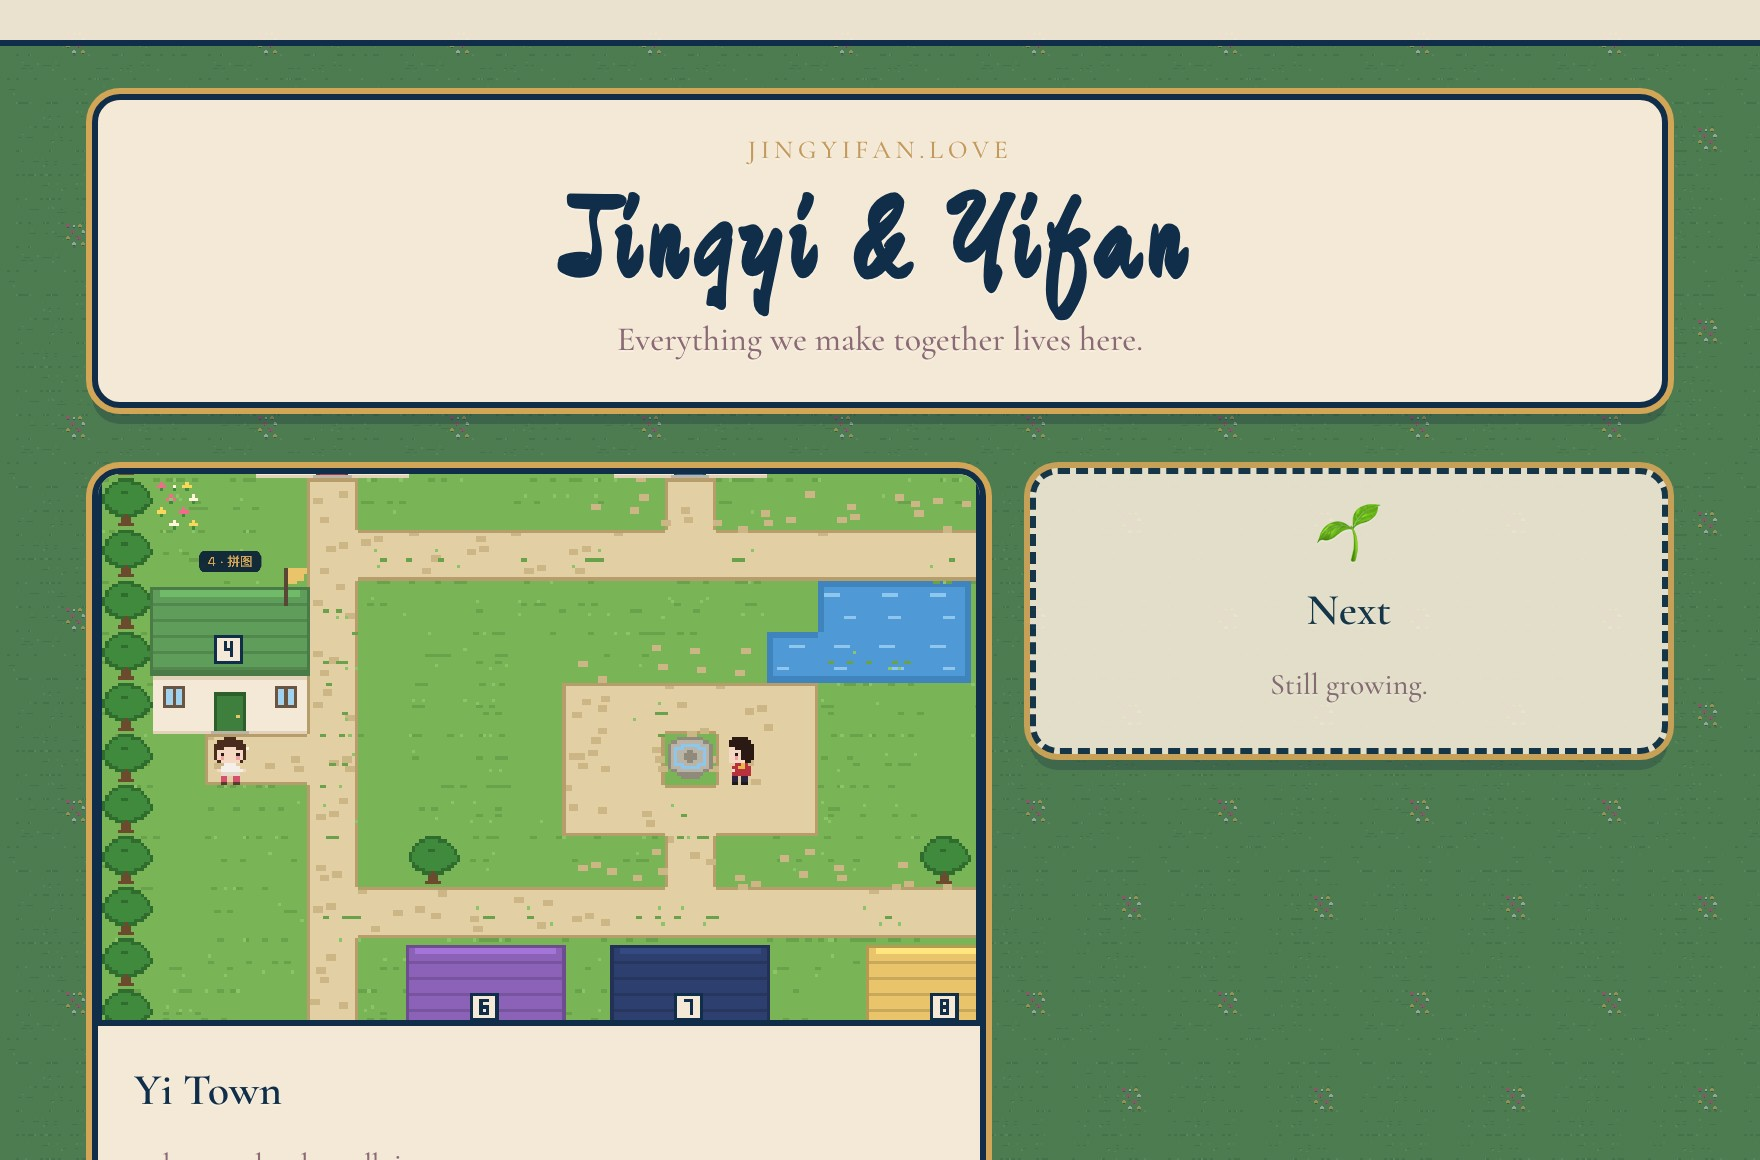
\includegraphics[width=\linewidth]{figures/page-dashboard.jpg}\caption{Dashboard}\end{subfigure}\hfill
  \begin{subfigure}[b]{0.49\columnwidth}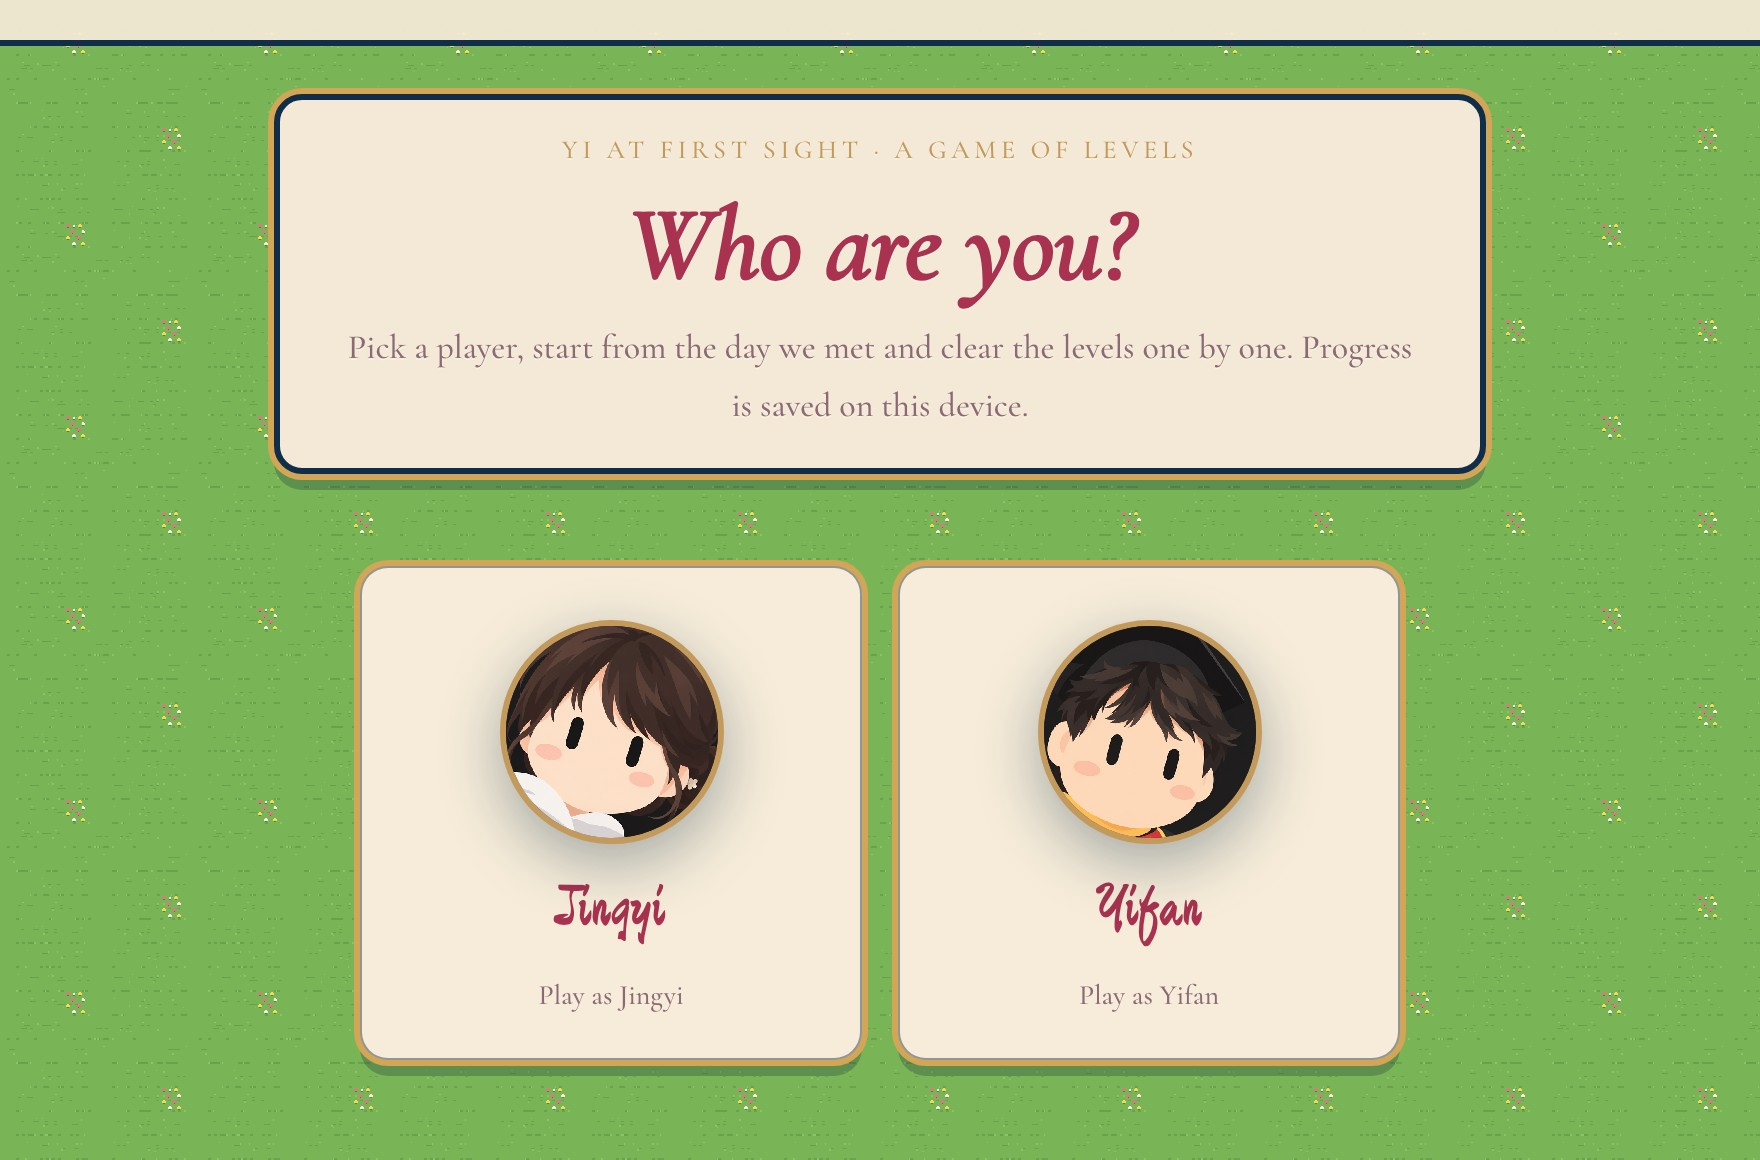
\includegraphics[width=\linewidth]{figures/page-start.jpg}\caption{Pick a player}\end{subfigure}\\[3pt]
  \begin{subfigure}[b]{0.49\columnwidth}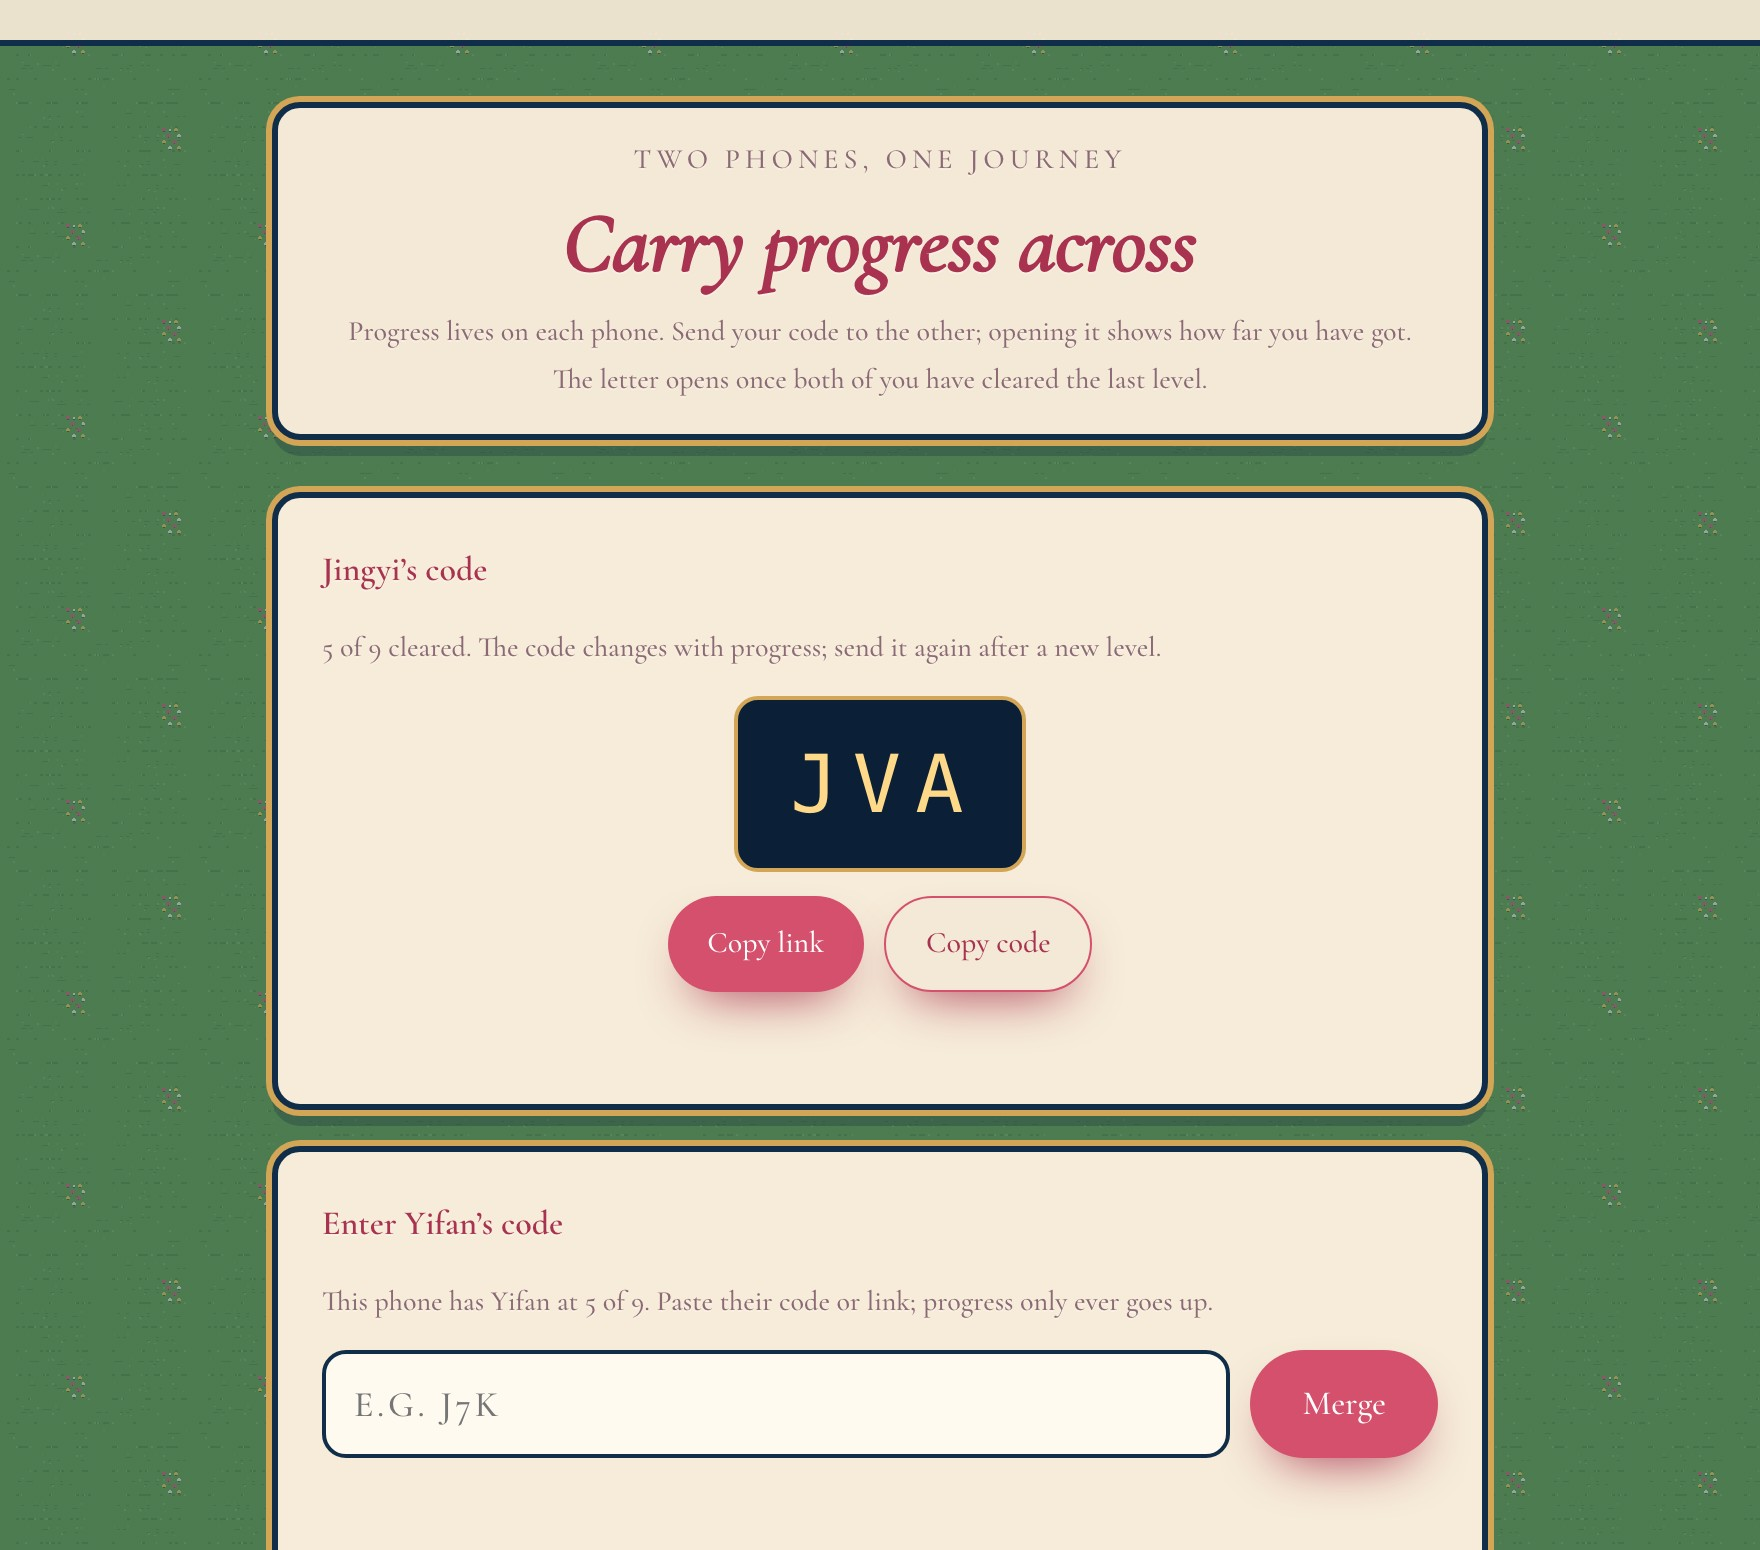
\includegraphics[width=\linewidth]{figures/page-sync.jpg}\caption{Progress code}\end{subfigure}\hfill
  \begin{subfigure}[b]{0.49\columnwidth}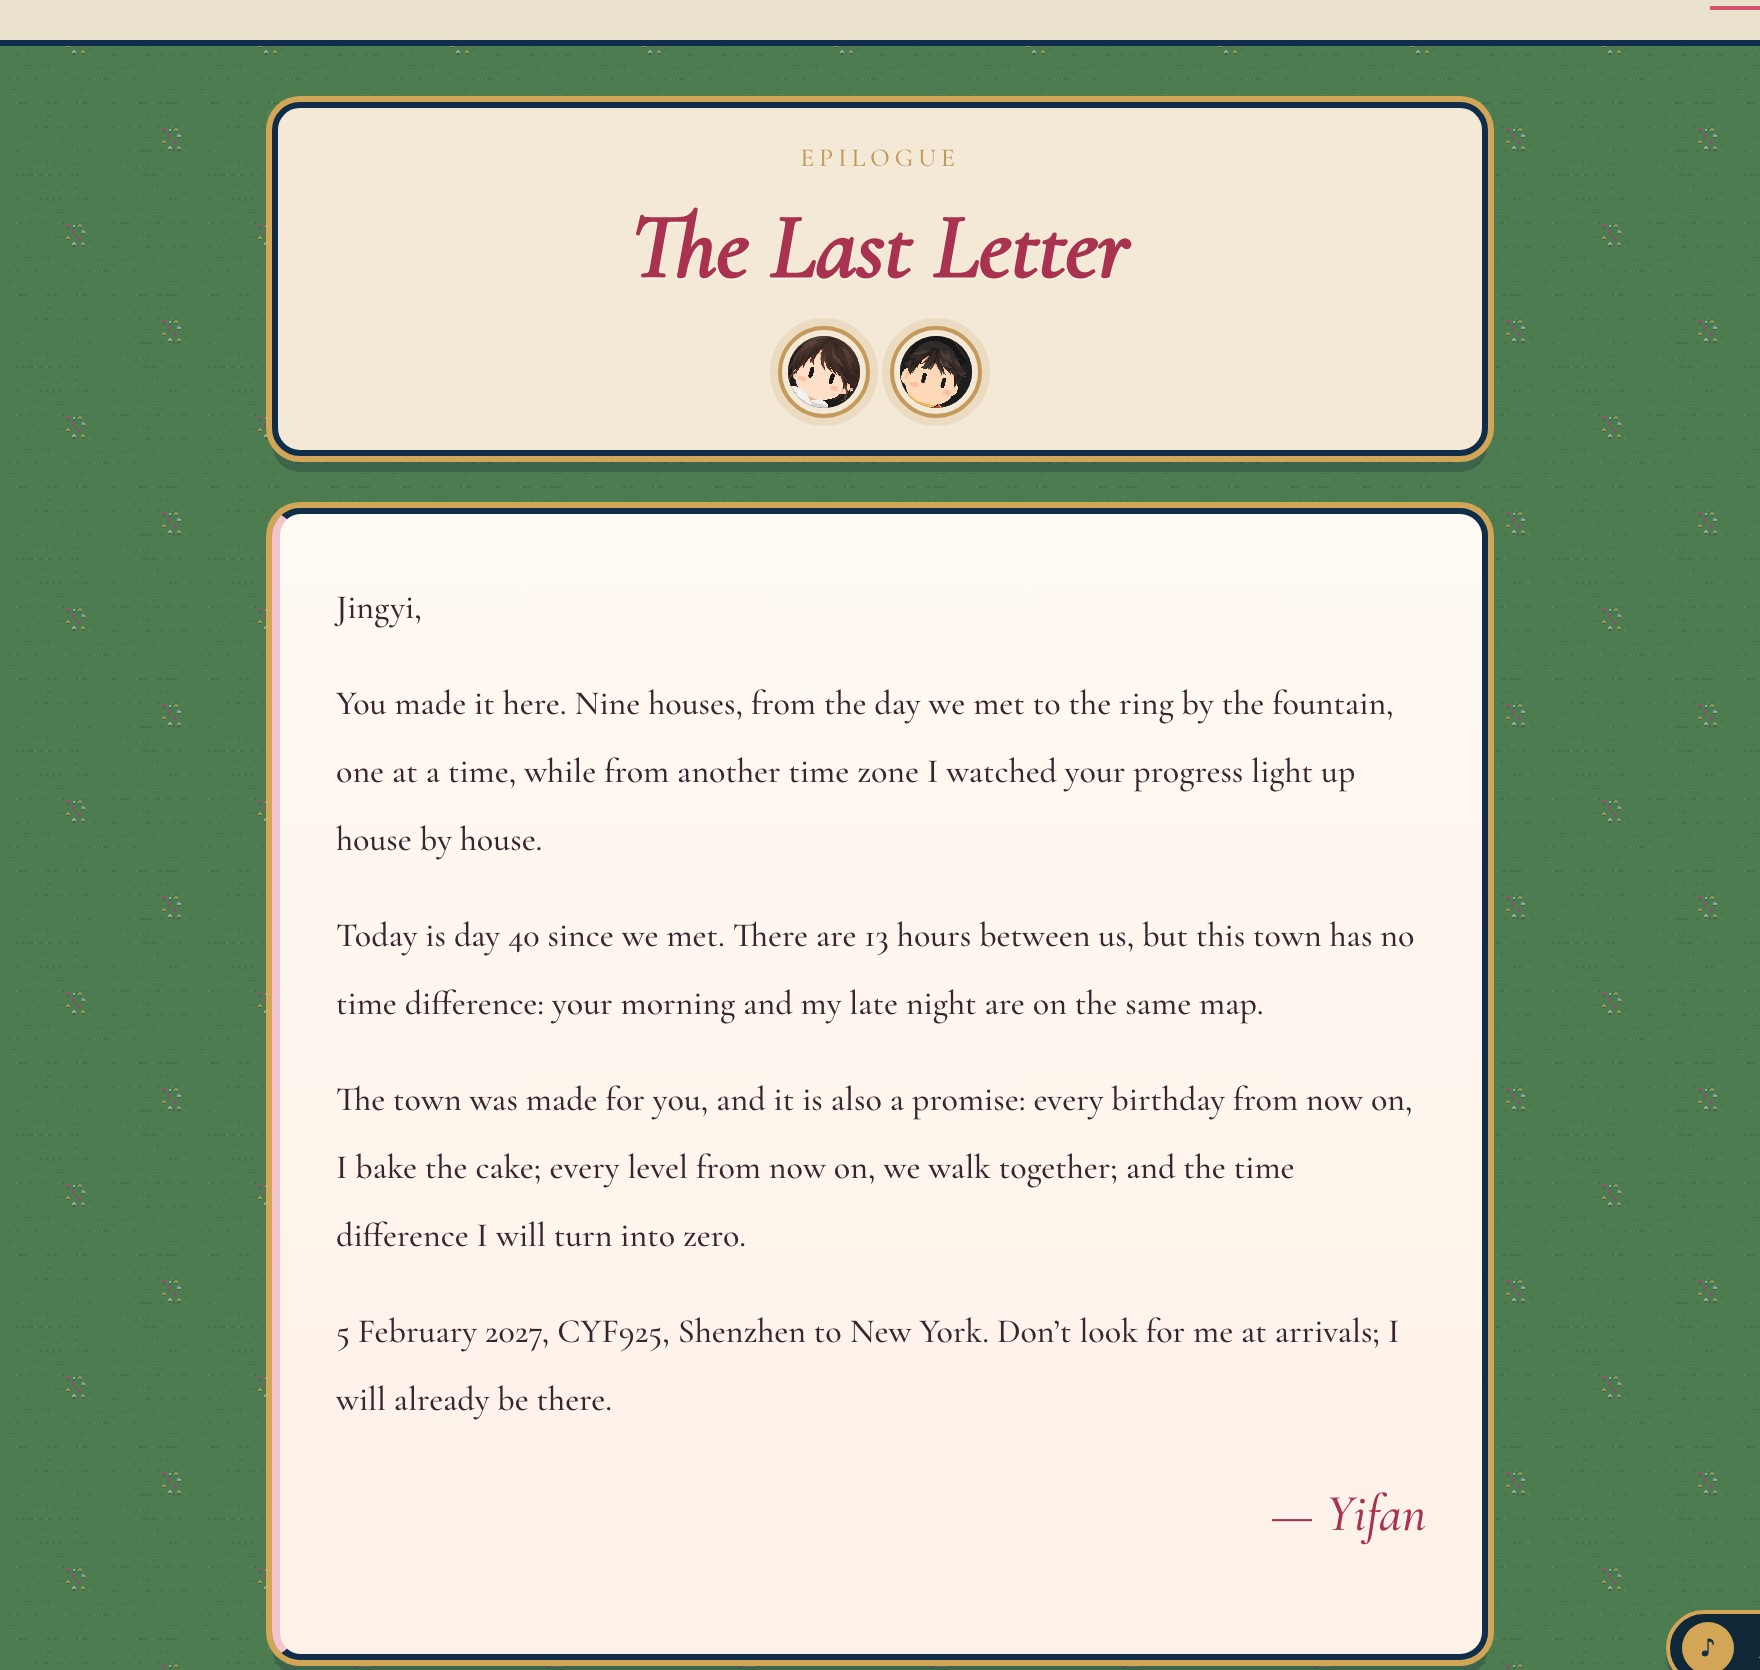
\includegraphics[width=\linewidth]{figures/page-letter.jpg}\caption{The last letter}\end{subfigure}
  \caption{Around the town. (a) The dashboard lists every product under the domain. (b) Each device
  keeps one progress per player. (c) Progress crosses phones as a code (here \code{JVA}). (d) The
  epilogue opens once both players have cleared the last level.}
  \Description{Four screenshots in cream and navy on a green pixel meadow: a dashboard card with a
  map thumbnail; two avatar cards; a large three-letter code; a handwritten-style letter.}
  \label{fig:front}
\end{figure}

\subsection{The town}
The town (Figure~\ref{fig:teaser-map}) is a $24\times20$ grid of $16\times16$-pixel tiles. Paths
connect nine houses around a fountain square and a pond. Each roof has its own colour and its
level number, and a cleared house flies a gold flag. The player moves with the arrow keys, by
tapping a tile (the avatar walks a shortest path to it), or with an on-screen d-pad. Walking into
a door opens a talk box with the level's one-line story, for example ``Our first game was on a Zoom
whiteboard. Now you place the last stone.''

Four kinds of character live in the town (Figure~\ref{fig:sprites}). The \emph{partner} waits by
the fountain and reports how far they have got (``I am waiting here. I have cleared 5 levels.
You?''). \emph{Rayford}, Yifan in a suit, is a scripted guide south of the fountain: he explains
the project, lists the levels, hints at the next one and walks the player to its door. Two Ragdoll
cats, \emph{Coffee} (\zh{咖啡}) and \emph{Duoduo} (\zh{哆哆}), guard the locks: Coffee sits at the next
locked door and Duoduo at the one after. When a door opens they walk to their new posts, and with
nothing left to guard they sunbathe by the pond. Bumping into a cat shows a photo of the real cat.
Two signposts lead out of the square to the two cities (Section~\ref{sec:days}), and a red mailbox
holds voice notes the partner has left.

The sky follows the clock in the player's own city: Jingyi walks the town in Shenzhen time and
Yifan in College Station time, so at the same instant one sees noon and the other sees lit windows
under a night wash. The whole site stands on the same pixel meadow, and every heading is a cream
sign in the town's palette, so leaving a house never leaves the world.

\begin{figure}[t]
  \centering
  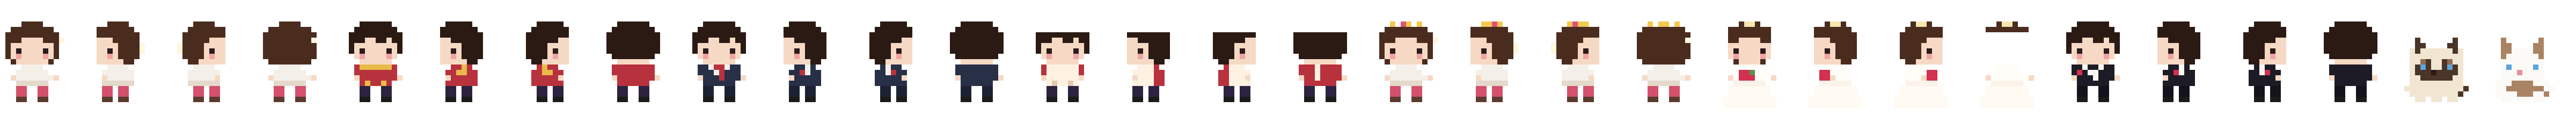
\includegraphics[width=\columnwidth]{figures/art-sprites.png}
  \caption{Every character in \yt{} is a string of characters in the source. From left: Jingyi,
  Yifan, Rayford, Yifan as the baker, Jingyi crowned, the bride and the groom (four facings each),
  then the cats Coffee and Duoduo. Bodies are $12\times12$ pixels over four rows of shared legs.}
  \Description{A row of tiny pixel-art characters seen from four sides, followed by two pixel cats.}
  \label{fig:sprites}
\end{figure}

\subsection{Nine levels}
Table~\ref{tab:levels} lists the levels with their source memory, mechanic and input modality,
and Figure~\ref{fig:levels} shows them in play.

\begin{table*}[t]
  \caption{The nine levels: each is a memory turned into a rule (\dc{1}). Modalities: \emph{V}~voice,
  \emph{T}~touch or pointer, \emph{C}~camera, \emph{K}~keyboard alternative available.}
  \label{tab:levels}
  \small
  \begin{tabular}{@{}clp{0.25\textwidth}p{0.36\textwidth}cl@{}}
    \toprule
    \# & Level & Source memory & Task (clear condition) & Input & Data \\
    \midrule
    1 & The Day We Met & 20 September 2026; the vow & Answer a question, then say \emph{\zh{我爱你，<name>，我愿意}} aloud; homophones of the name accepted & V/K & 1 vow per player \\
    2 & Love Map & Where each studied; where they will meet & Name six street views; each right answer drops a heart on the map to collect & T & 6 places \\
    3 & Tattoo & A promise to write on each other & Handwrite a line on an arm or shoulder, then ``ink it'' & T & strokes \\
    4 & Moments & The first 40 days & Order five memories, then reassemble a $3\times3$ portrait of the partner & T & 8 memories \\
    5 & Gomoku & First game on a Zoom whiteboard & Ten win-in-one endgames; the ten answers form a heart & T & 10 positions \\
    6 & Our Songs & The six songs they share & Hear a passage, pick the title from four & T & 6 songs \\
    7 & Libra and Scorpius & Their birth signs, neighbours in the sky & Join 22 stars along 20 edges & T/K & J2000 positions \\
    8 & Us, in Old Verse & Classical love poetry & Restore the missing half-line of five poems character by character & T & 5 poems \\
    9 & Meridian & What comes next & Try the ring on through the camera and take a photo & C & 3 GLB models \\
    \bottomrule
  \end{tabular}
\end{table*}

\begin{figure*}[t]
  \centering
  \begin{subfigure}[b]{0.24\textwidth}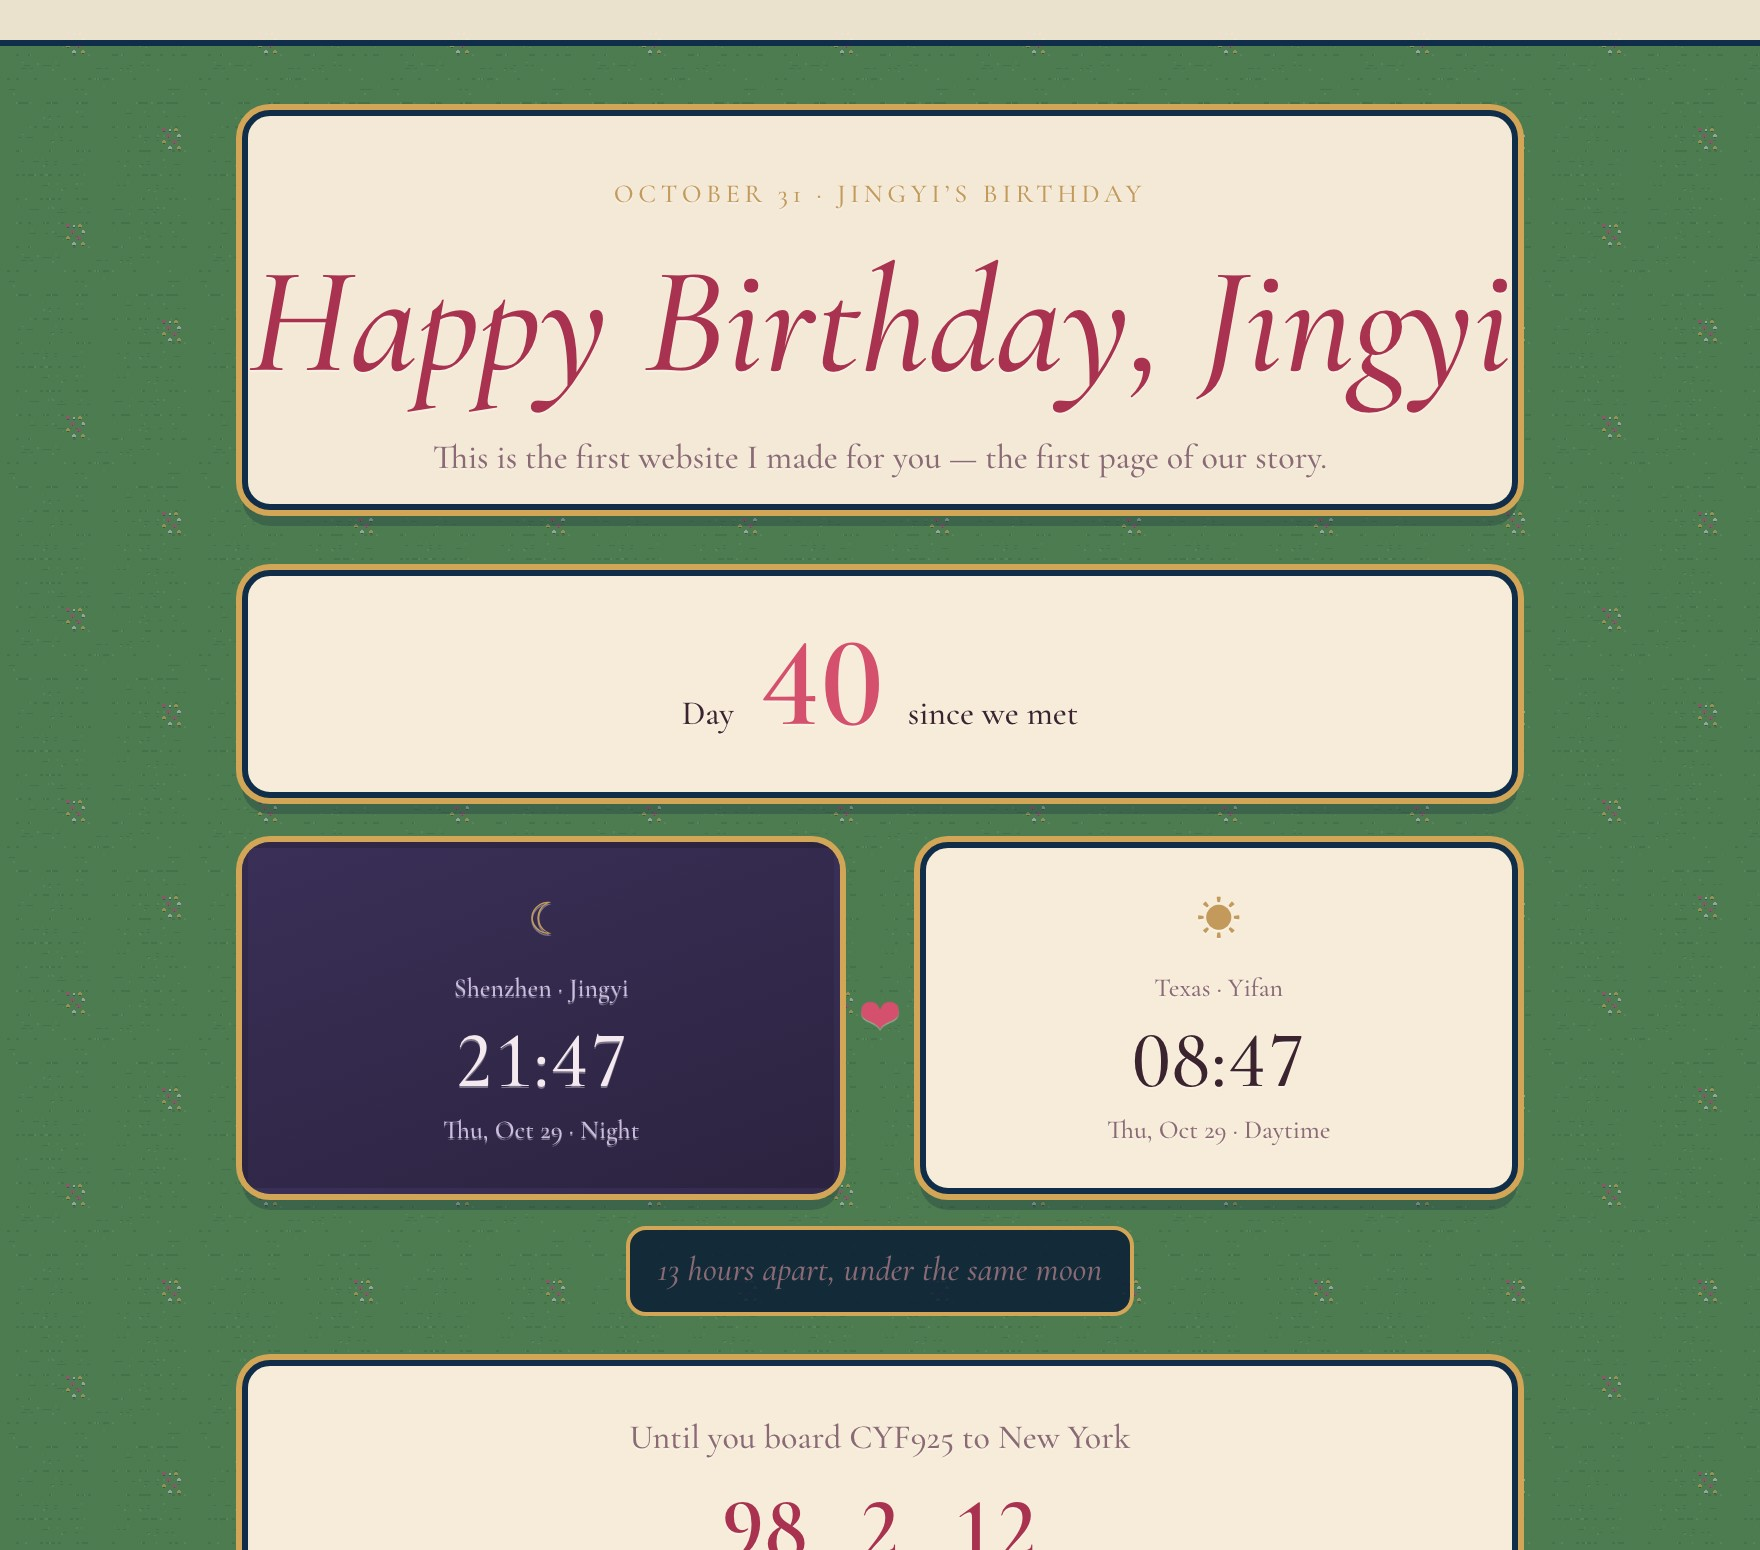
\includegraphics[width=\linewidth]{figures/page-met.jpg}\caption{1 The Day We Met}\end{subfigure}\hfill
  \begin{subfigure}[b]{0.24\textwidth}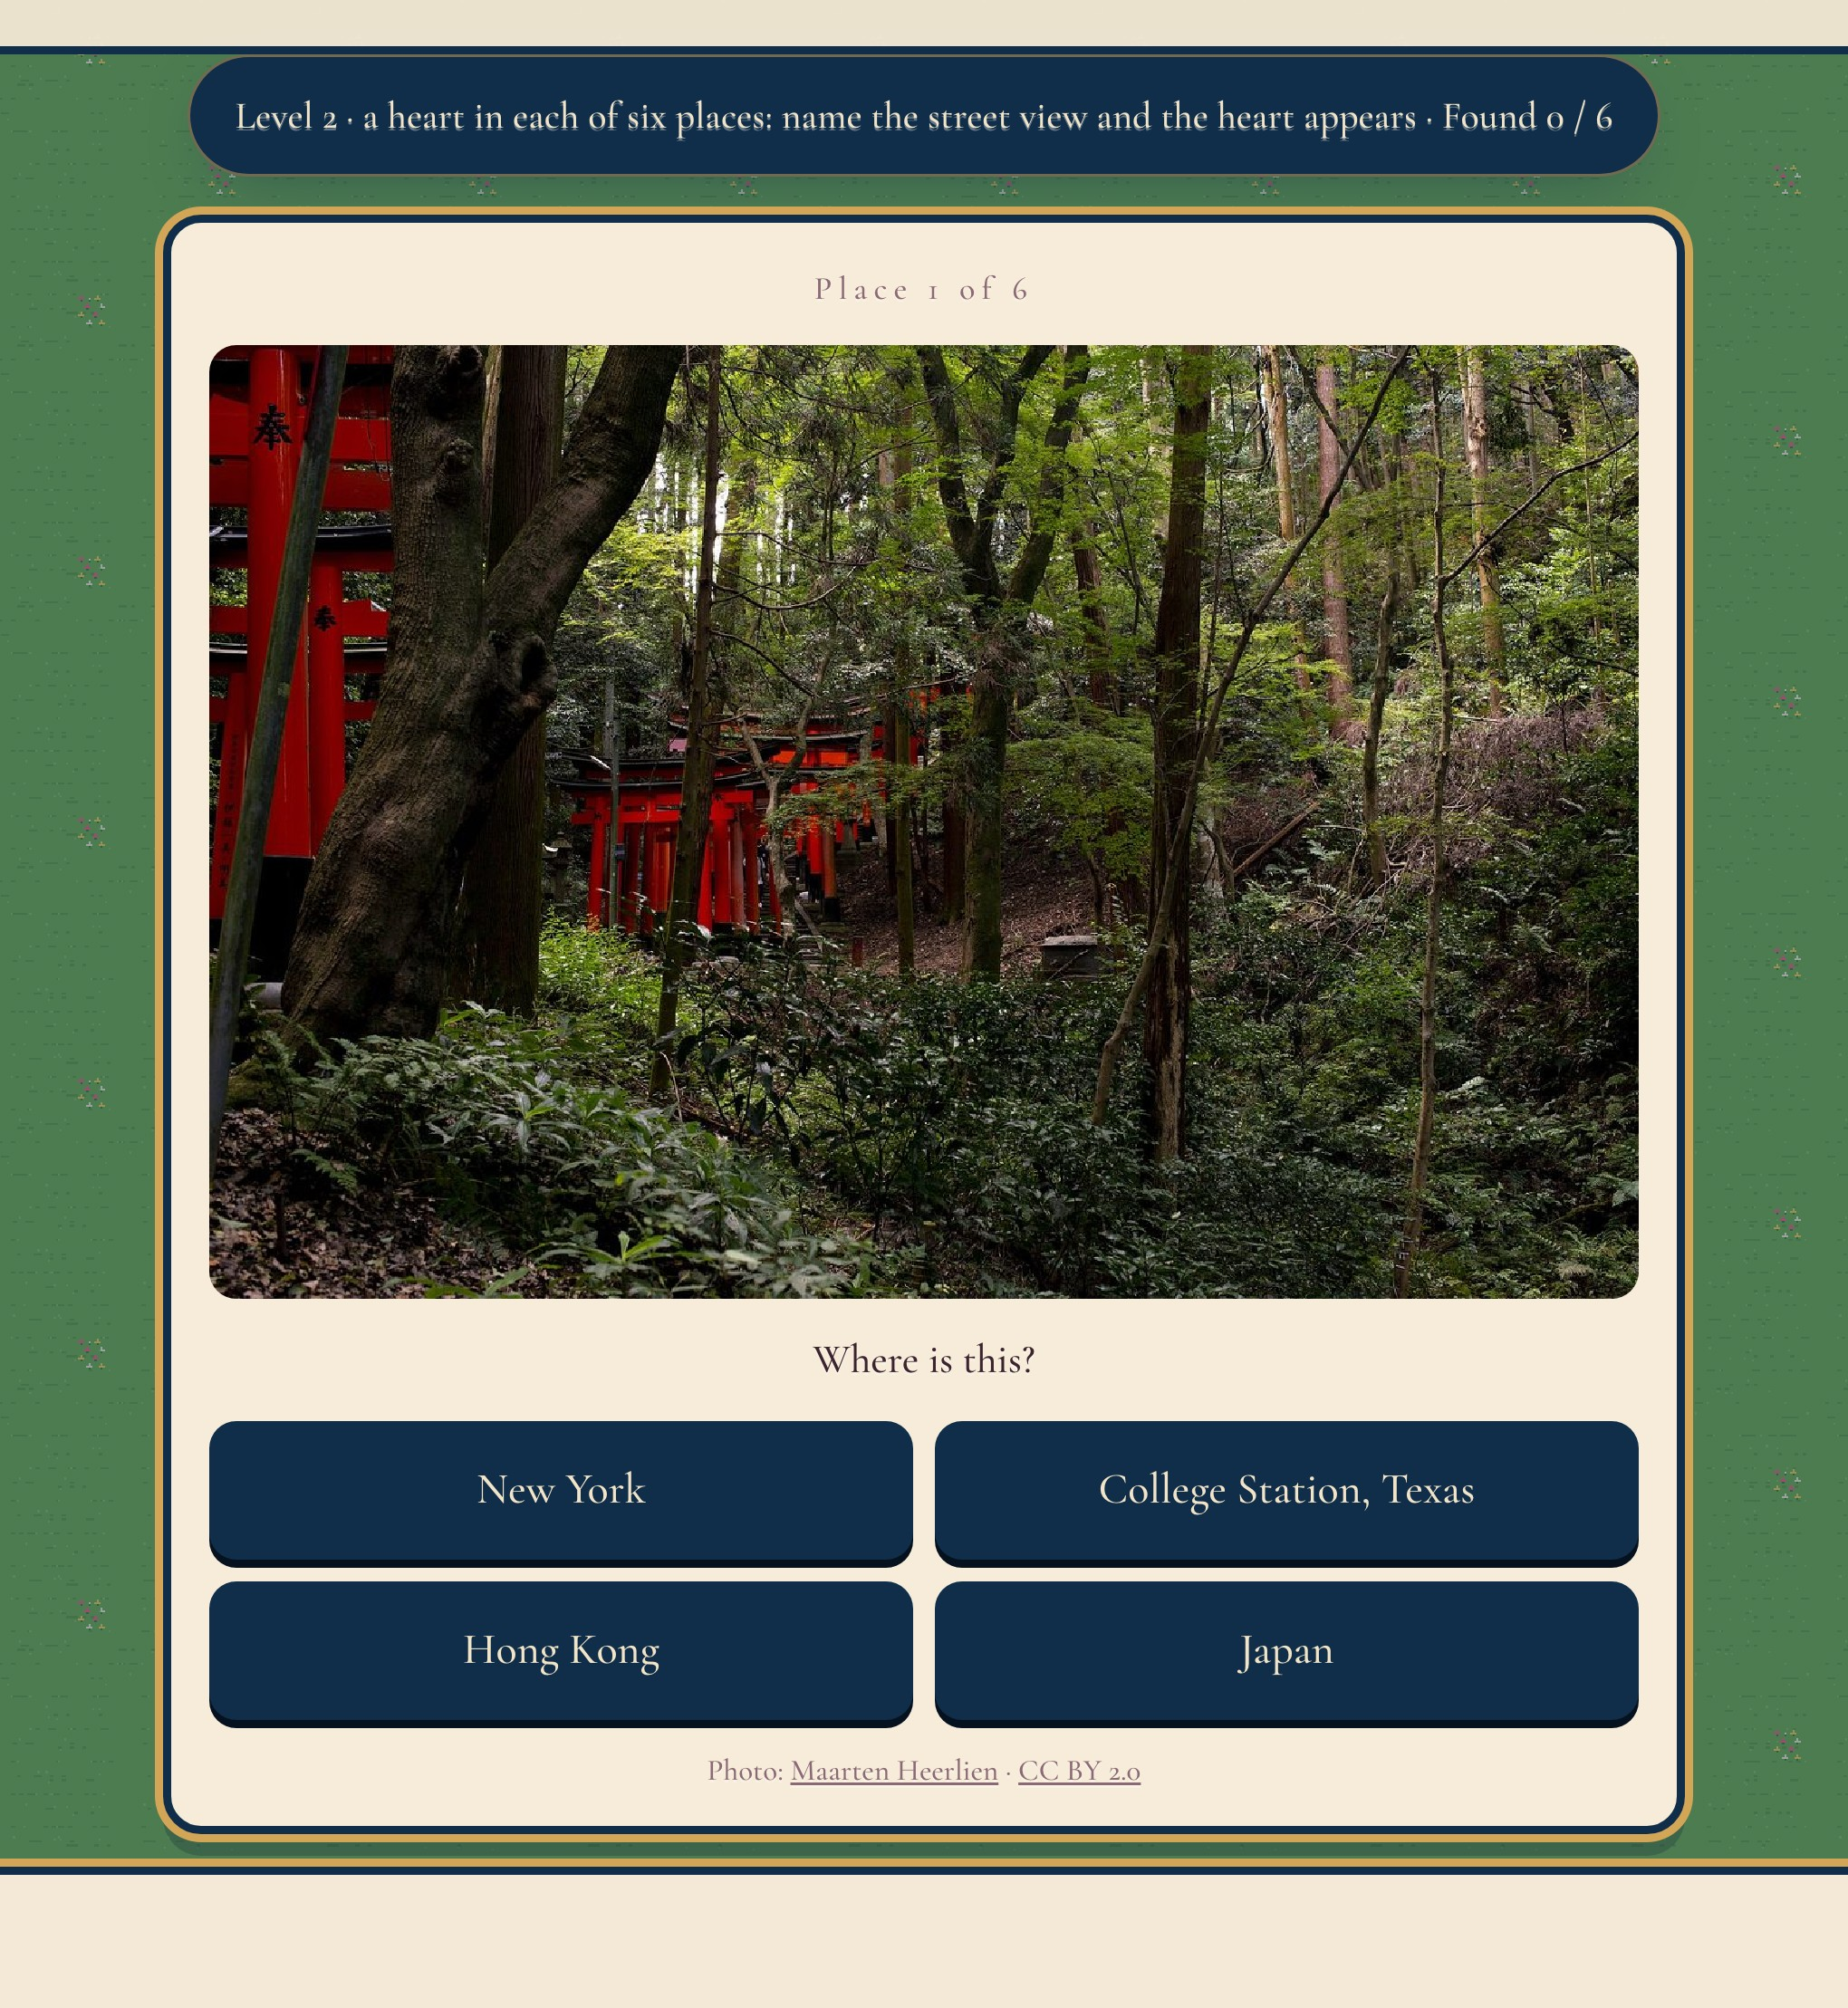
\includegraphics[width=\linewidth]{figures/page-map.jpg}\caption{2 Love Map}\end{subfigure}\hfill
  \begin{subfigure}[b]{0.24\textwidth}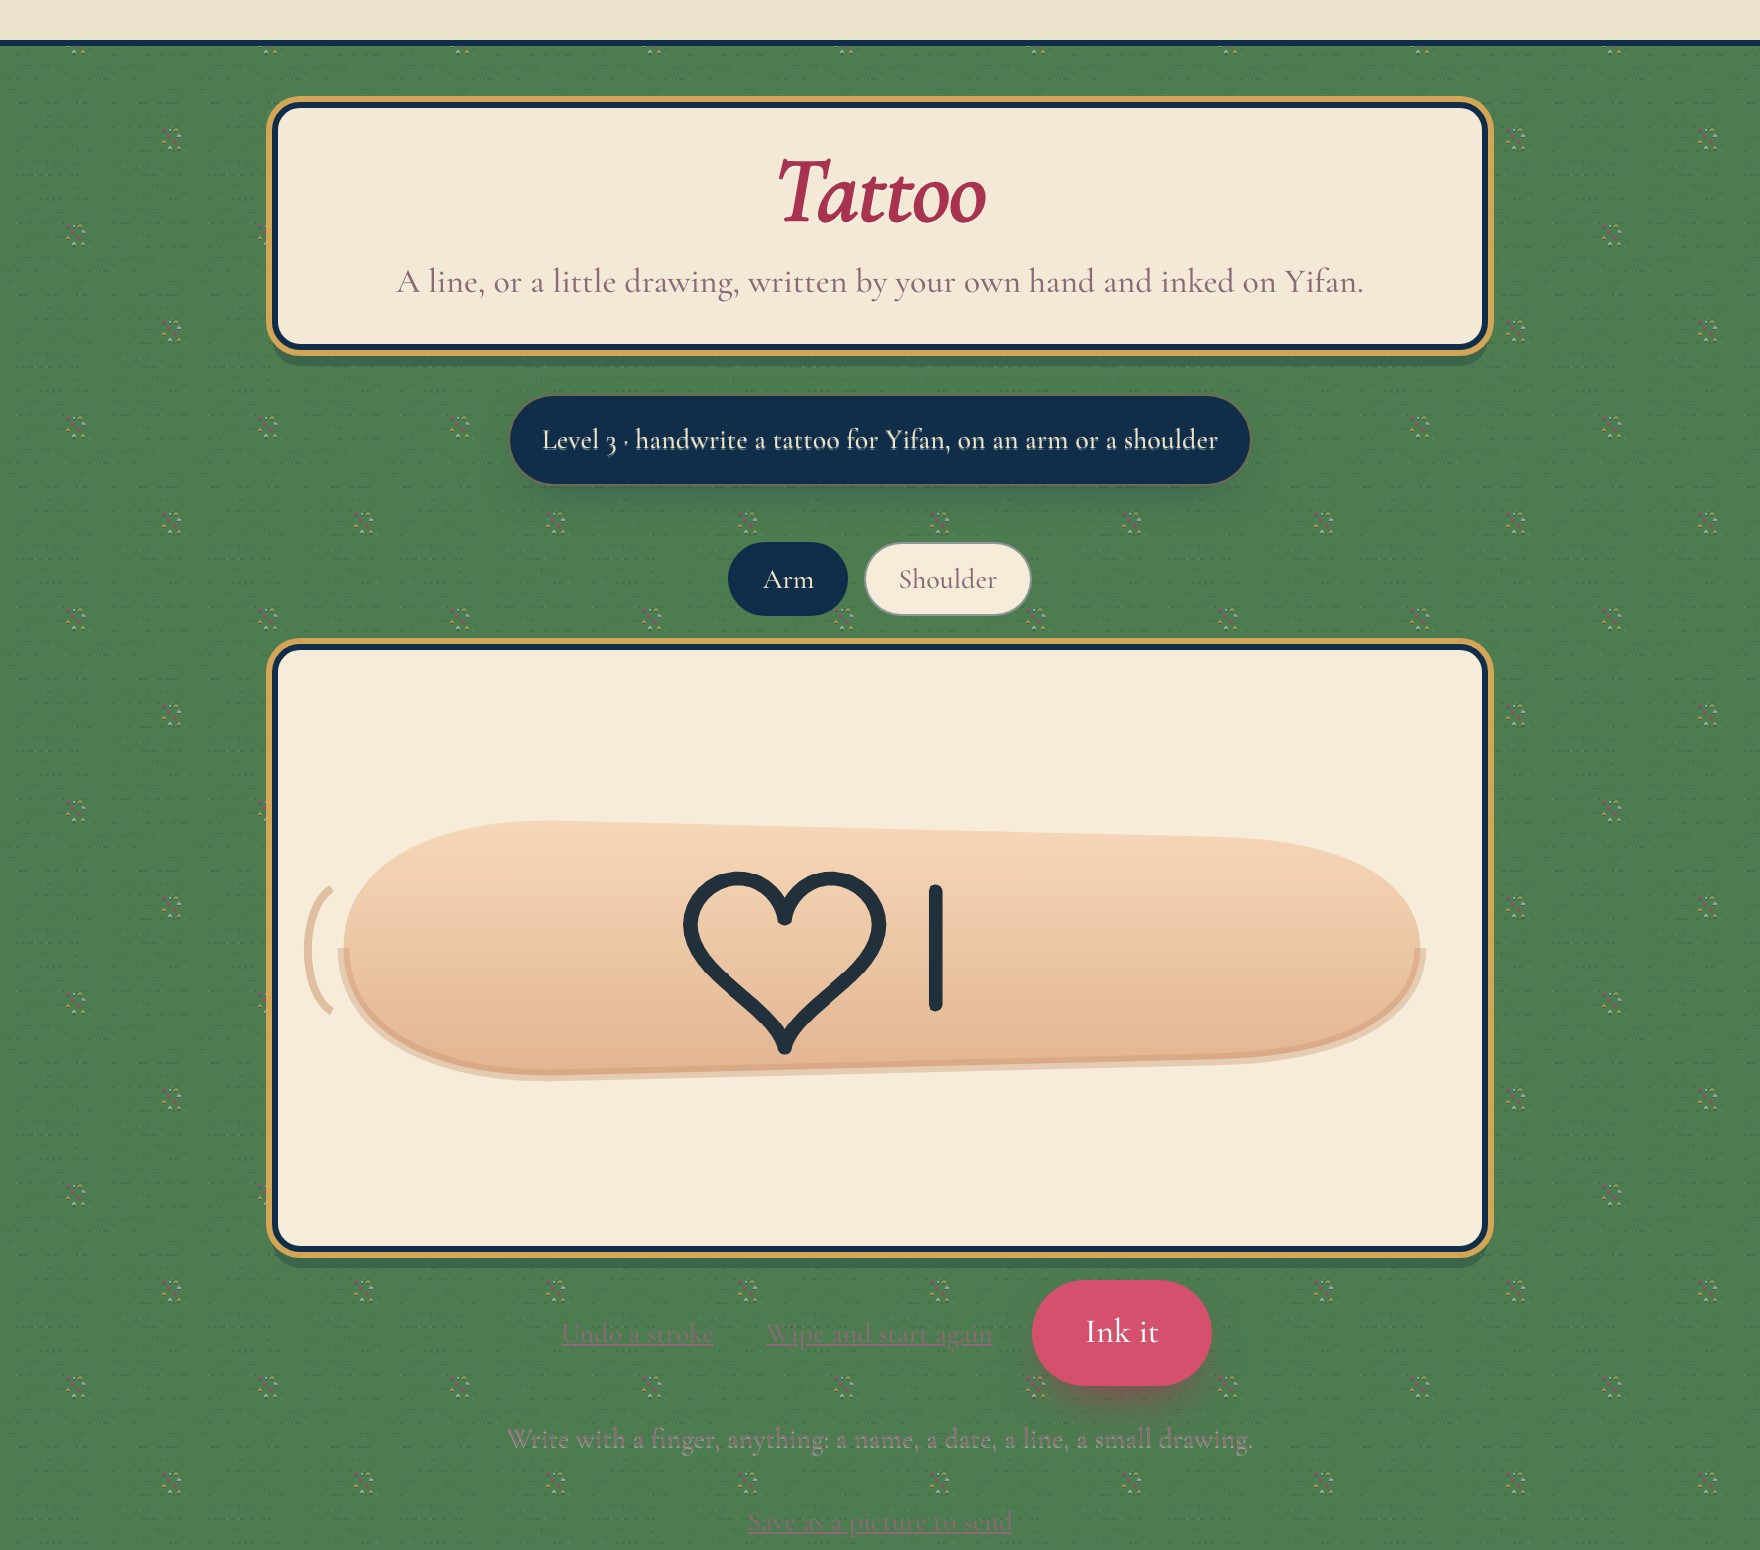
\includegraphics[width=\linewidth]{figures/page-tattoo.jpg}\caption{3 Tattoo}\end{subfigure}\hfill
  \begin{subfigure}[b]{0.24\textwidth}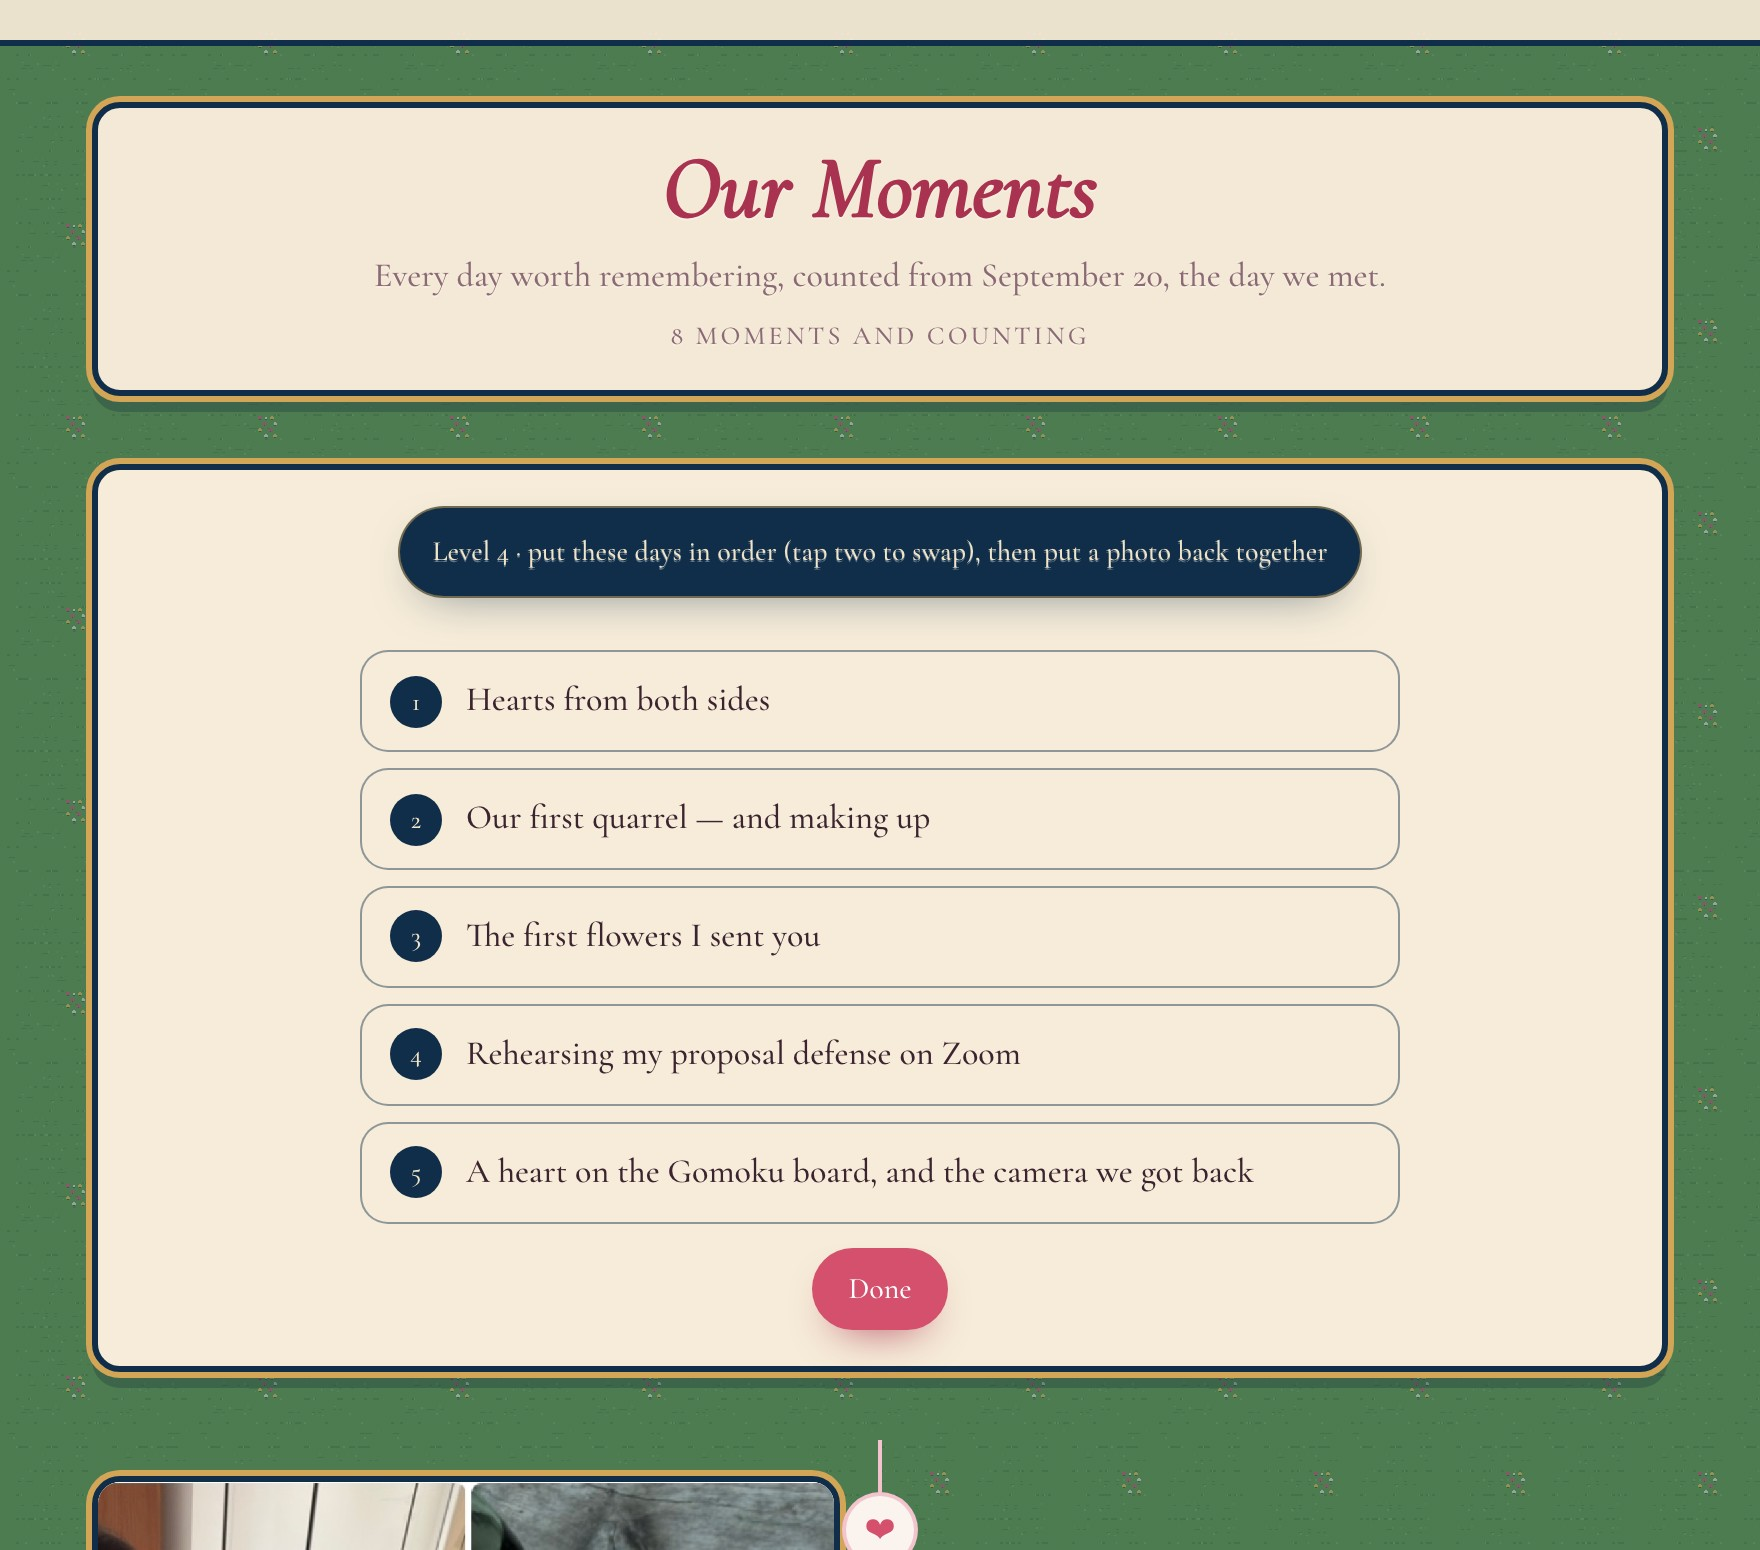
\includegraphics[width=\linewidth]{figures/page-moments.jpg}\caption{4 Moments}\end{subfigure}\\[4pt]
  \begin{subfigure}[b]{0.24\textwidth}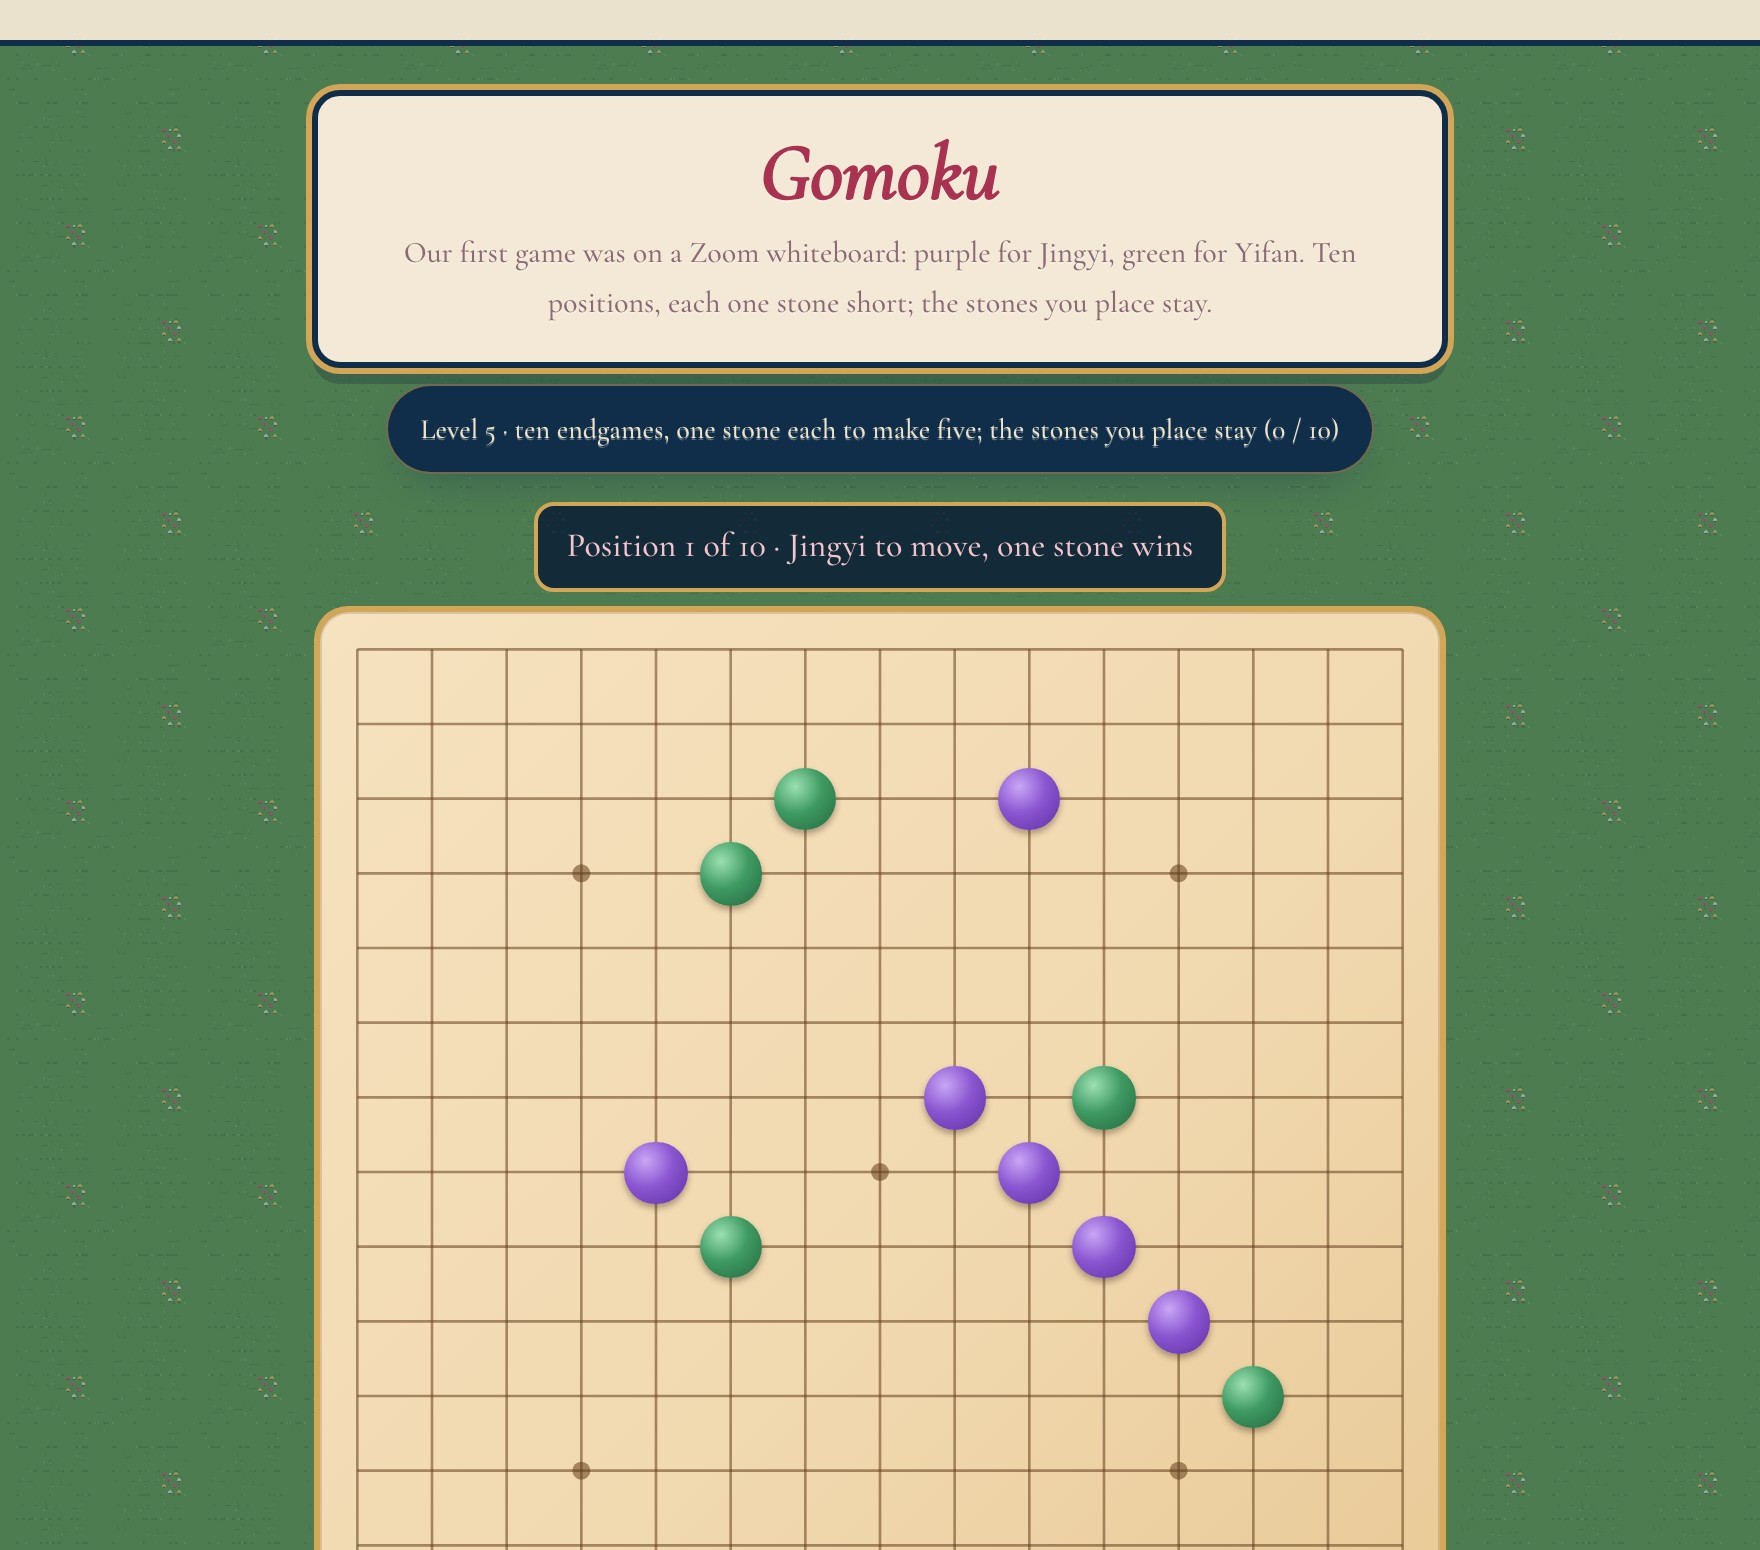
\includegraphics[width=\linewidth]{figures/page-gomoku.jpg}\caption{5 Gomoku}\end{subfigure}\hfill
  \begin{subfigure}[b]{0.24\textwidth}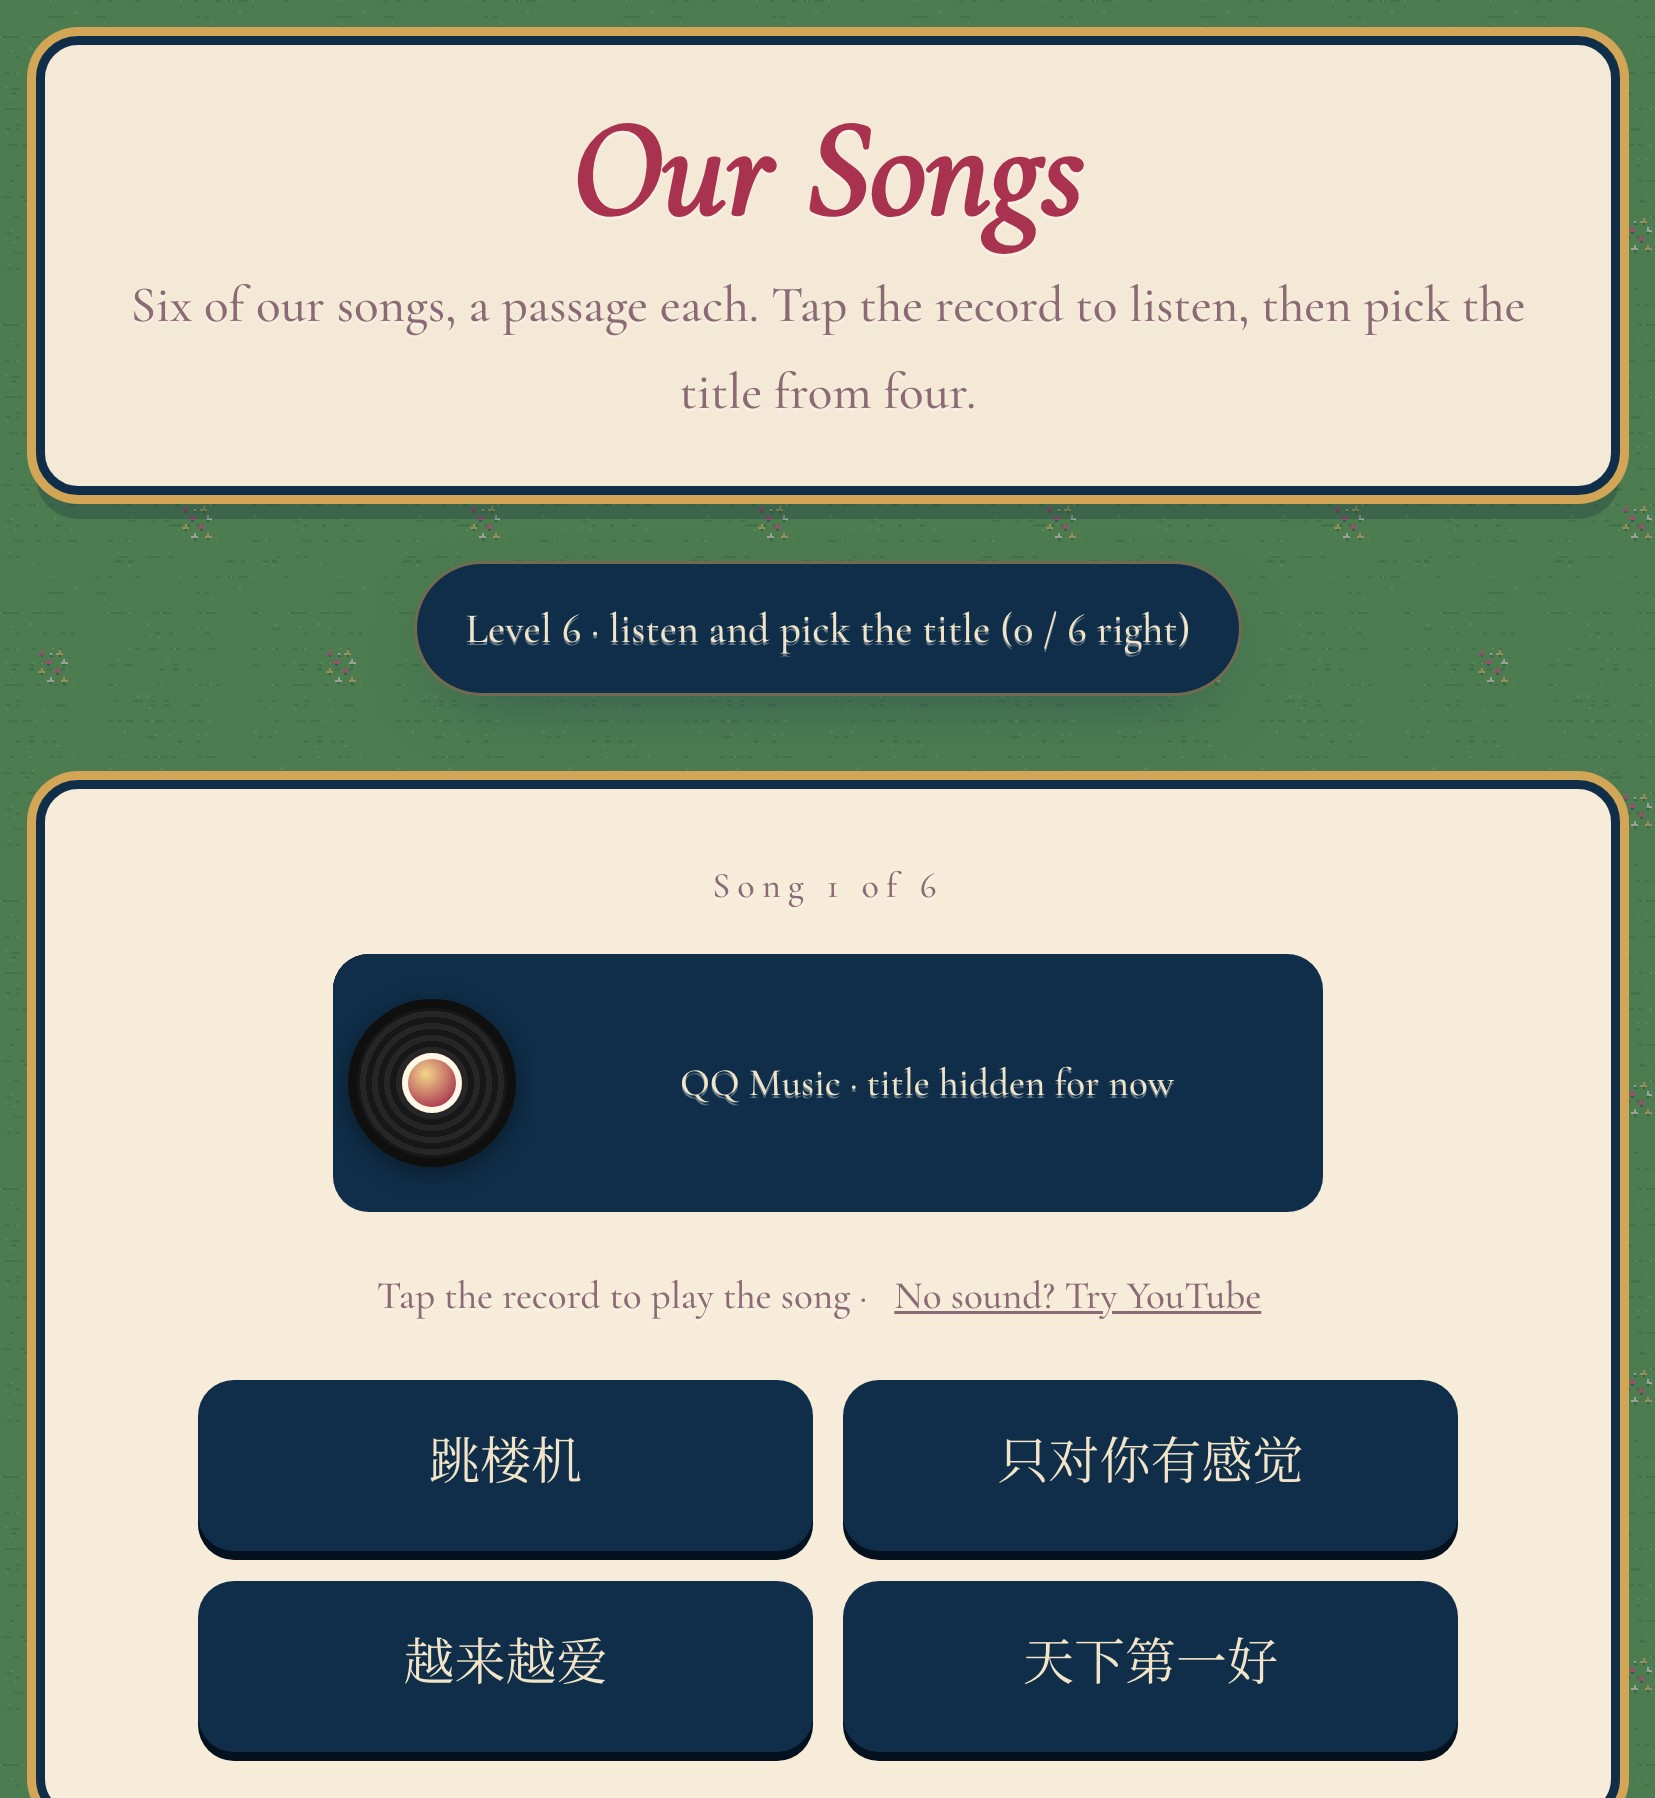
\includegraphics[width=\linewidth]{figures/page-songs.jpg}\caption{6 Our Songs}\end{subfigure}\hfill
  \begin{subfigure}[b]{0.24\textwidth}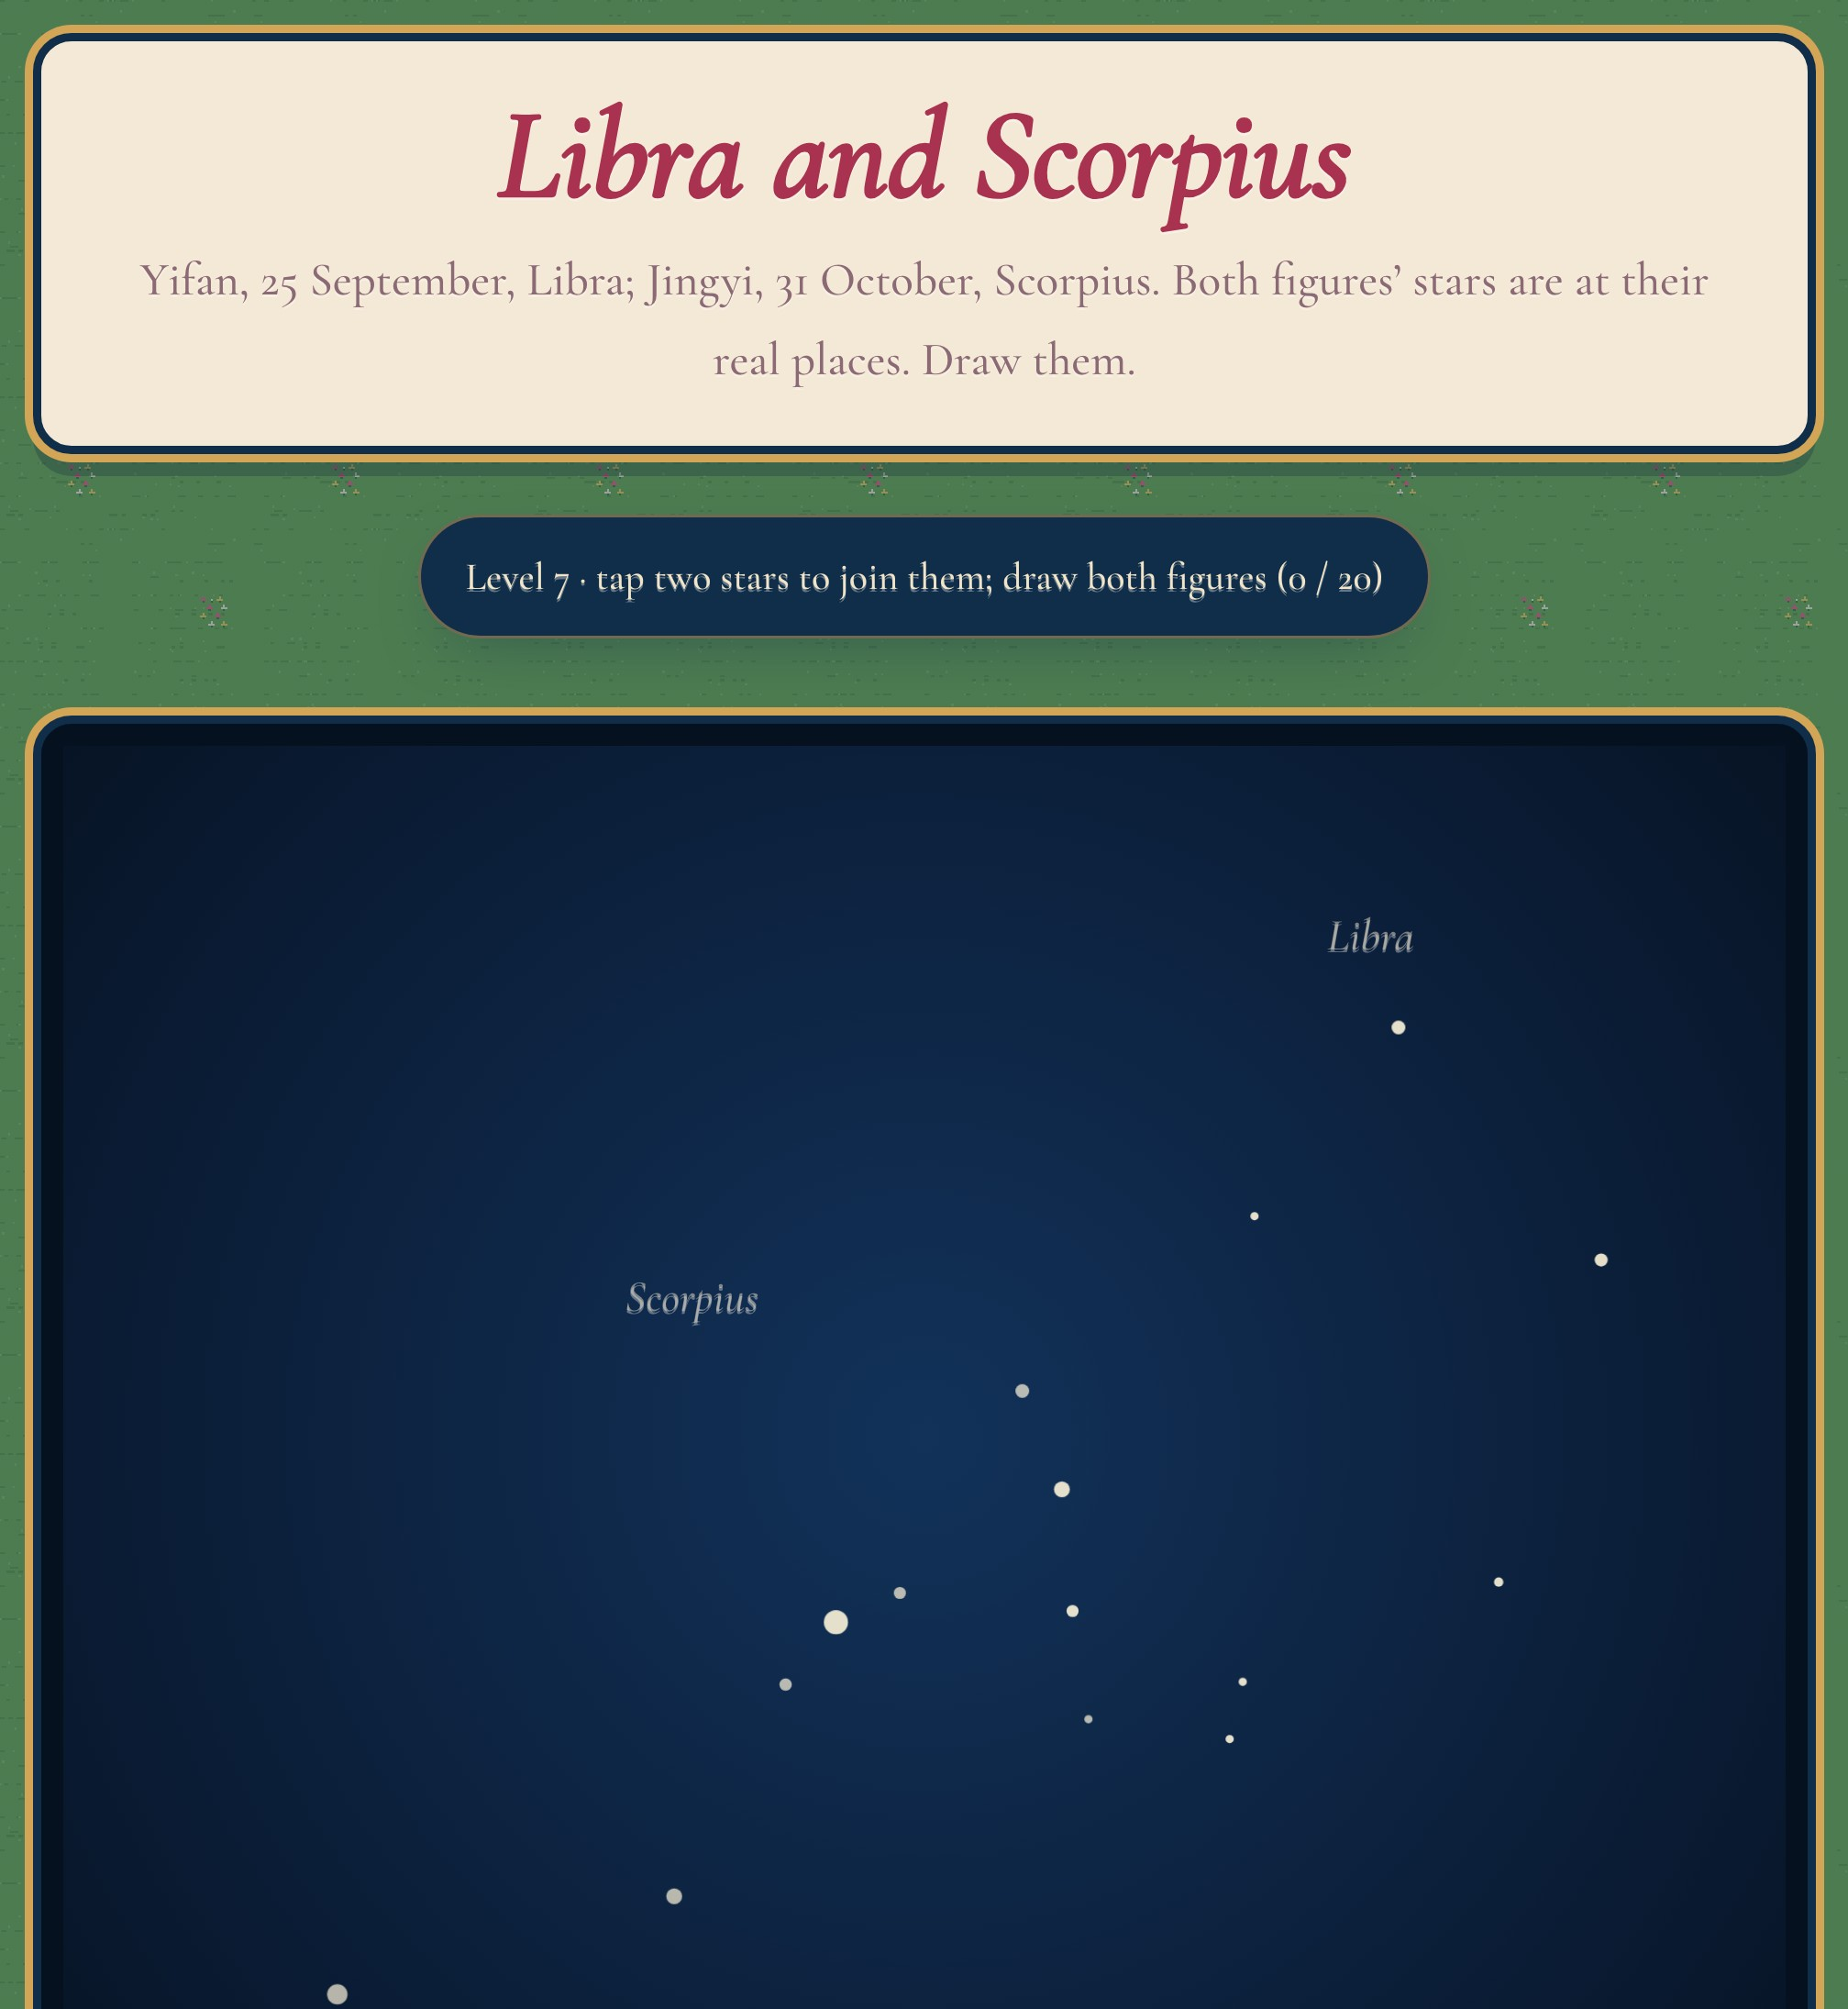
\includegraphics[width=\linewidth]{figures/page-stars.jpg}\caption{7 Libra and Scorpius}\end{subfigure}\hfill
  \begin{subfigure}[b]{0.24\textwidth}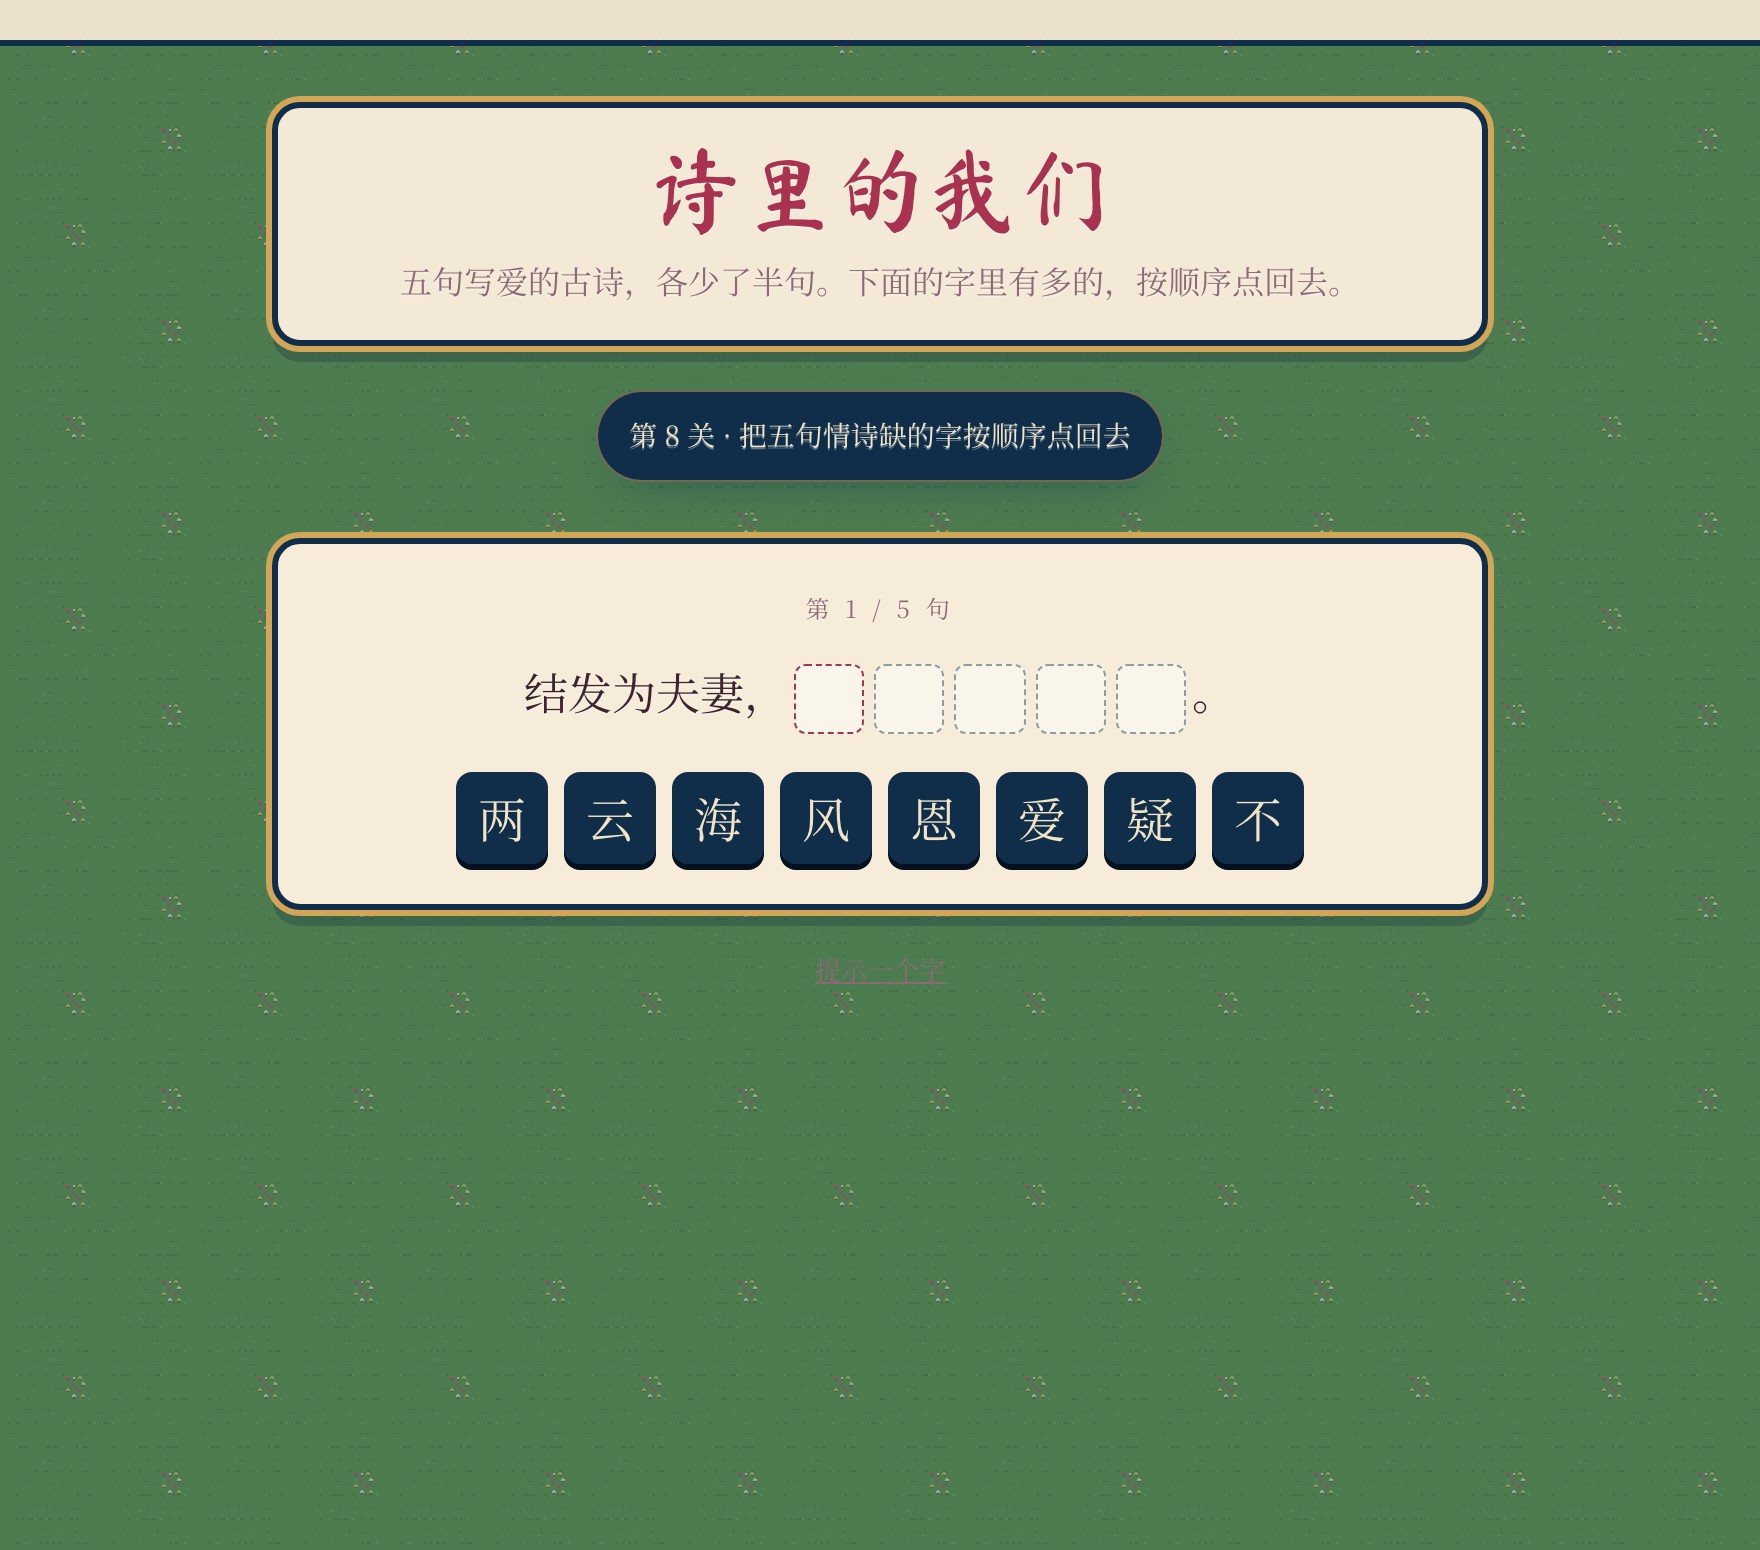
\includegraphics[width=\linewidth]{figures/page-poems.jpg}\caption{8 Us, in Old Verse}\end{subfigure}
  \caption{Eight of the nine levels in play (the ninth is shown in Figure~\ref{fig:ring}). (a) Day
  counter, twin clocks and the countdown to CYF925. (b) Name the place in the street view. (c)~A
  heart inked on an arm. (d) Put the first days in order. (e) Position~1 of~10: one stone wins.
  (f)~Name the song. (g) Libra's ``claws'' and Scorpius, before they are joined. (h) Su Wu's line
  \kai{结发为夫妻，恩爱两不疑} with its second half to restore.}
  \Description{Eight screenshots of the levels, each a cream panel on green pixel grass.}
  \label{fig:levels}
\end{figure*}

\paragraph{1. The Day We Met.} The first level shows the day count since 20 September, the time
in both cities with day and night icons, and a countdown to the flight. To clear it, each player
reads a vow, rewritten from the wedding formula as the vow of ``becoming each other's partner
once more'', and says one line aloud: \zh{我爱你，陈静仪，我愿意} (``I love you, Jingyi Chen, I do''),
with the partner's full name. Browser speech recognition~\cite{w3c2023speech} hears Mandarin
names inconsistently, so the matcher removes everything except Han characters and Latin
letters and accepts any of eight or nine homophone spellings of each name (for example \zh{陈静怡},
\zh{陈静宜}). A typed fallback keeps the level playable in browsers that cannot listen.

\paragraph{2. Love Map.} Six places matter to the couple: Texas, Los Angeles, Japan, Shenzhen,
Hong Kong and New York. Before each heart appears on a Leaflet map, the player names a
street-level photograph from four options (Figure~\ref{fig:levels}b); a wrong pick reshuffles the
options. Great-circle arcs connect the two home cities.

\paragraph{3. Tattoo.} The player handwrites a line or a small drawing on an arm or a shoulder,
drawn in SVG, and inks it. The tattoo is kept on the device and can be saved as an image to send.

\paragraph{4. Moments.} The timeline holds eight dated memories, each with photos and a story in
both languages, from hearts made from both sides of the ocean (day~21) to a heart drawn on the
Gomoku board (day~35). The player orders five of them by tapping pairs to swap, then reassembles a
$3\times3$ portrait of the partner.

\paragraph{5. Gomoku.} Each of ten positions on a $15\times15$ board has exactly one winning point
for the player's own colour (purple for Jingyi, green for Yifan, as in their first game). The ten
answers are the ten points of a heart; solved answers stay on the board in gold, so the heart draws
itself as the player progresses. Positions are generated from three patterns (a four closed at one
end, a broken four, three-and-one) placed around each heart point in varied directions with decoy
stones, and a test checks that each has a unique winning move. Gomoku is a first-player win under
optimal play~\cite{allis1994searching}; win-in-one puzzles avoid that question entirely and make
every move feel like a find.

\paragraph{6. Our Songs.} Six songs the couple share (among them \zh{只对你有感觉} and
\zh{天下第一好}) play a passage through the official embedded players: QQ Music for the player in
China and YouTube for the player in the United States, each switchable. The site hosts no audio.
The options unlock only after the passage has been heard.

\paragraph{7. Libra and Scorpius.} Yifan is a Libra (25 September) and Jingyi a Scorpio
(31 October); in the sky the two constellations are neighbours, and Libra's two brightest stars
still bear the Arabic names of the Scorpion's claws, \emph{Zubenelgenubi} and
\emph{Zubeneschamali}. The level projects 22 stars from J2000 coordinates and
magnitudes~\cite{meeus1998astronomical} and asks the player to draw both figures, 20 edges in all.

\paragraph{8. Us, in Old Verse.} Five classical lines about love lose their second half, to be
restored from a bank of characters: Su Wu's farewell to his wife, \kai{结发为夫妻，恩爱两不疑};
Guan Daosheng's \emph{Song of You and Me}; a couplet of Li Shangyin; the paired birds of the
sixth-century anthology \emph{New Songs from a Jade Terrace}~\cite{birrell1982jade}; and an
anonymous couplet. Each solved line shows a plain English gloss.

\paragraph{9. Meridian.} The last level is a pair of rings, called \emph{Meridian}, modelled
procedurally in Blender from a Python script (Figure~\ref{fig:ring}). The pair share a signature:
a yellow-gold line inlaid around a platinum band like a meridian on a globe, a hidden sapphire
inside the bottom, and an inner engraving that carries the \emph{other} person's name and birthday,
the date they met and the coordinates of the airport where they will meet ($40.64^\circ$N
$73.78^\circ$W). Her ring exists in two designs, a solitaire on four compass prongs (v1) and the
current flush-set stone sunk into his band's profile (v2); the page keeps both as a design history.
The level is cleared only one way: the player tries the ring on through the camera and takes a
photo (Section~\ref{sec:sensing}).

\begin{figure}[t]
  \centering
  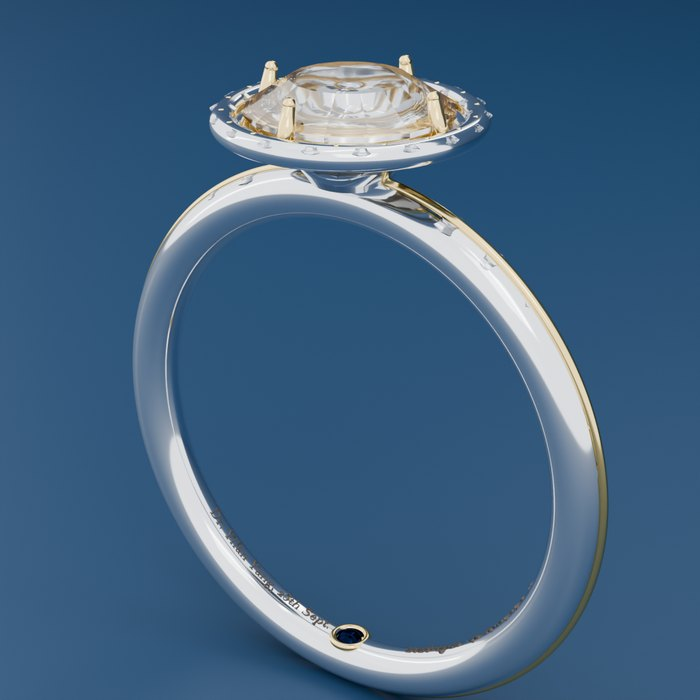
\includegraphics[width=0.325\columnwidth]{figures/hers_v1_hero.jpg}\hfill
  
\includegraphics[width=0.325\columnwidth]{figures/hers_hero.jpg}\hfill
  
\includegraphics[width=0.325\columnwidth]{figures/his_hero.jpg}
  \caption{The Meridian pair, path-traced from the procedural Blender model: hers v1 (solitaire,
  halo and graduated shoulder stones), hers v2 (flush-set 4.2\,mm stone in a 5\,mm flat band), and
  his (brushed flat comfort-fit band). The gold meridian runs around each band.}
  \Description{Three renders of rings on a dark background: a diamond solitaire, a flat band with
  a sunken stone, and a plain wide band, each with a thin gold line around it.}
  \label{fig:ring}
\end{figure}

\subsection{Two days}\label{sec:days}
Two signposts lead from the square to a day in each city (Figure~\ref{fig:days}). Each is a second
map with the person's stops: Yifan's home, gym, his advisor's office, the golf course and the
pool in College Station; Jingyi's home with the cats at the door, her drive, the office and
Shenzhen Bay. Each stop has hours, and the person's sprite stands wherever the clock in their own
city puts them. A partner who opens Yifan's day at 9:49 p.m. in Shenzhen finds him at 8:49 a.m. at
his advisor's office. The schedules began as guesses and were corrected by the owner: Yifan drives
rather than taking the bus; Jingyi drives a Tesla rather than taking the metro; and the
Shenzhen Bay stop keeps a joke between them about where they will one day live.

\begin{figure}[t]
  \centering
  \begin{subfigure}[b]{0.49\columnwidth}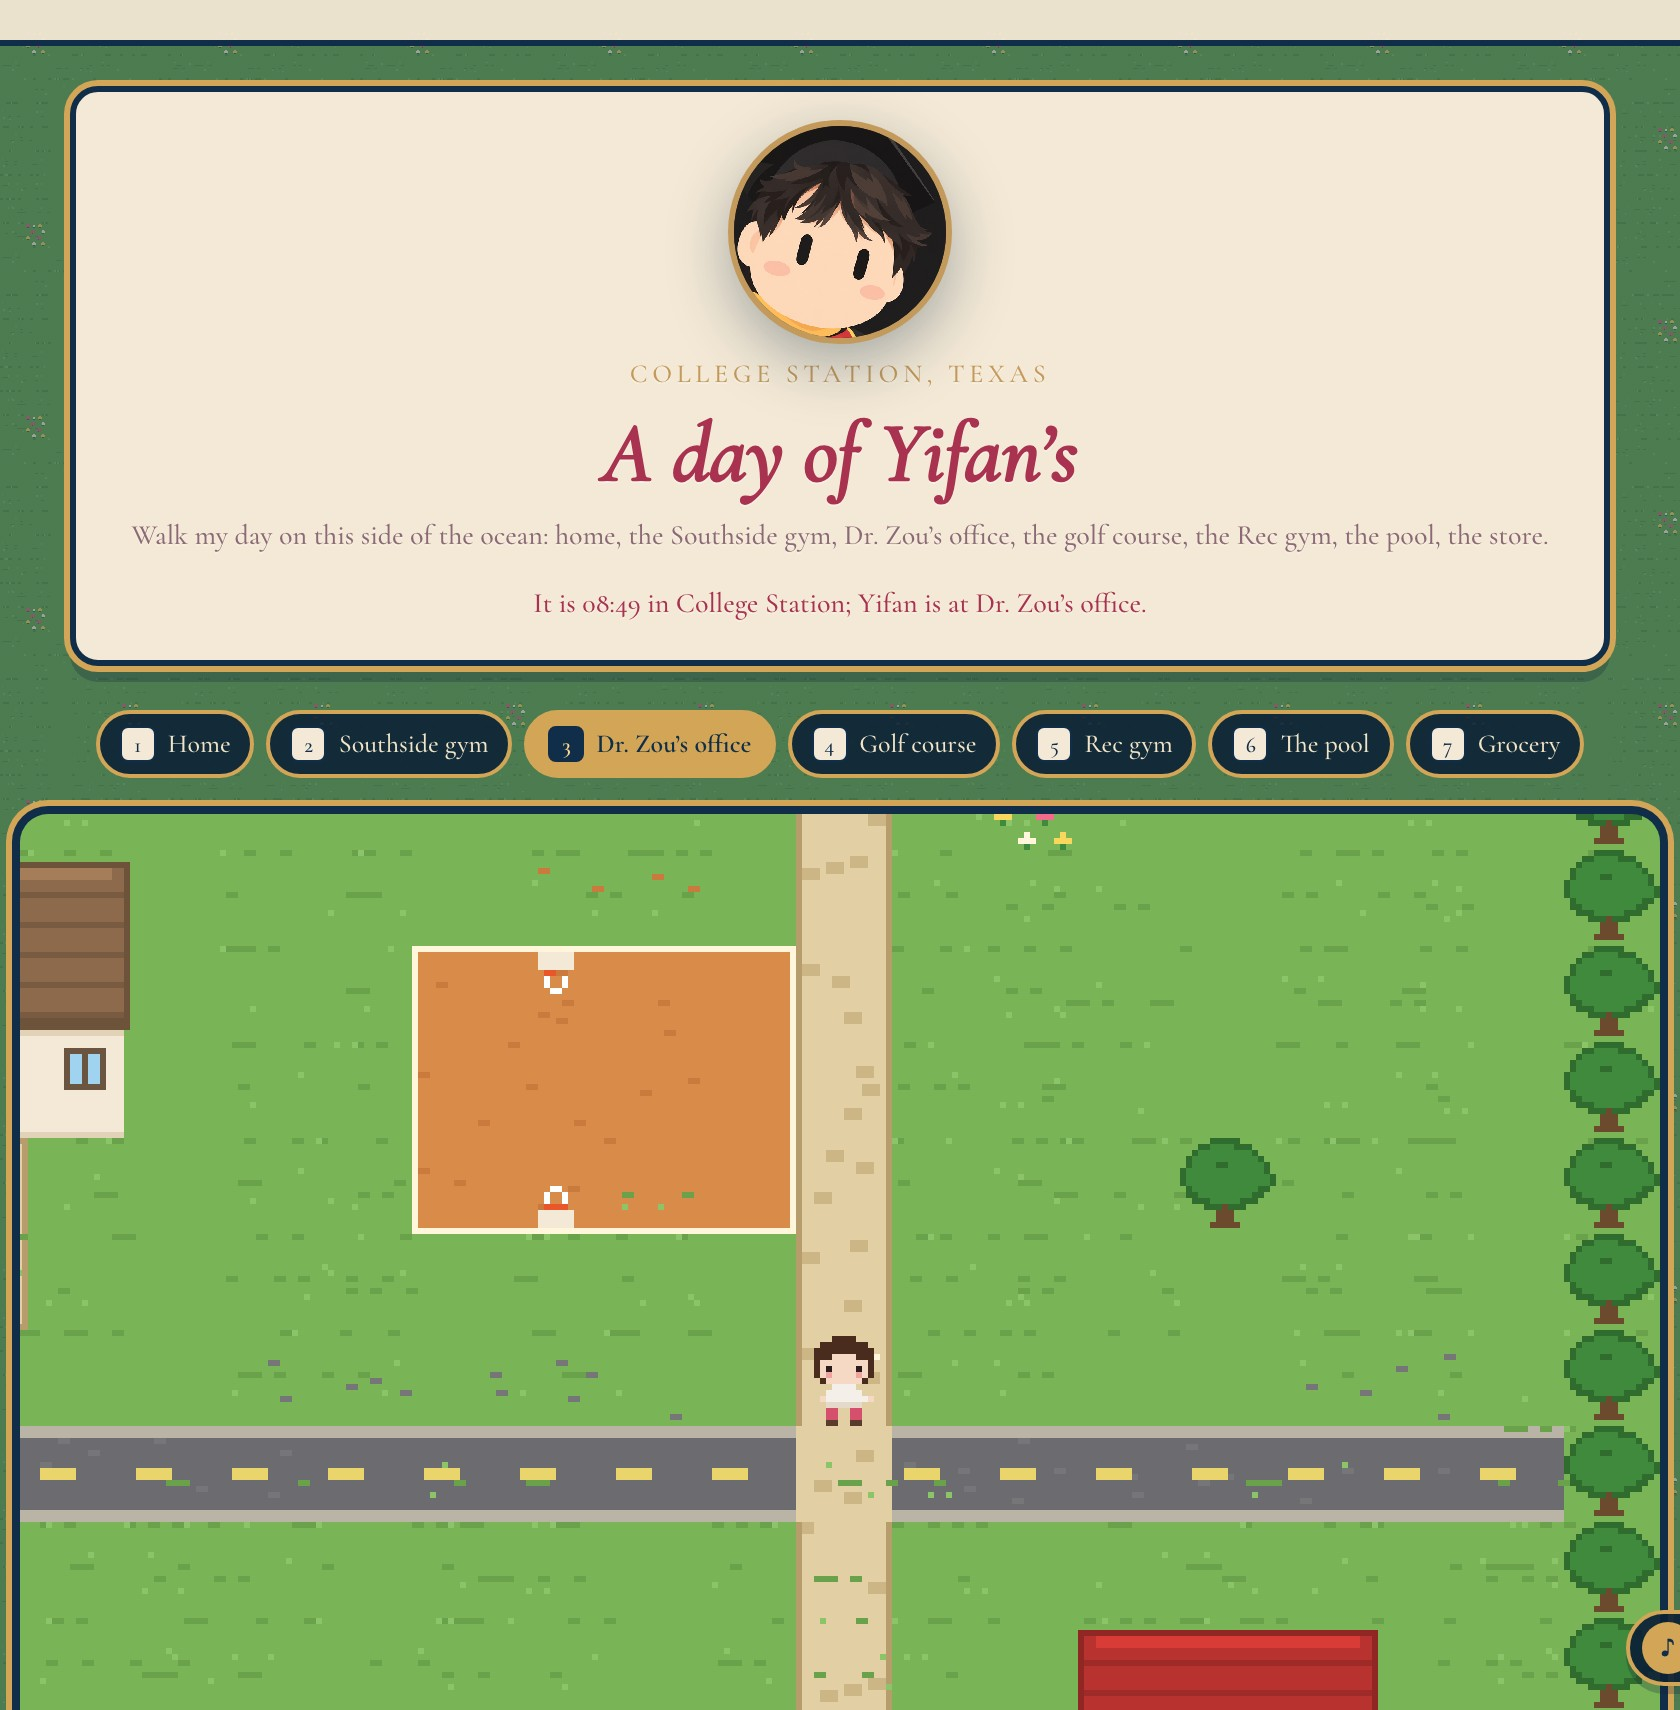
\includegraphics[width=\linewidth]{figures/page-cs.jpg}\caption{A day of Yifan's}\end{subfigure}\hfill
  \begin{subfigure}[b]{0.49\columnwidth}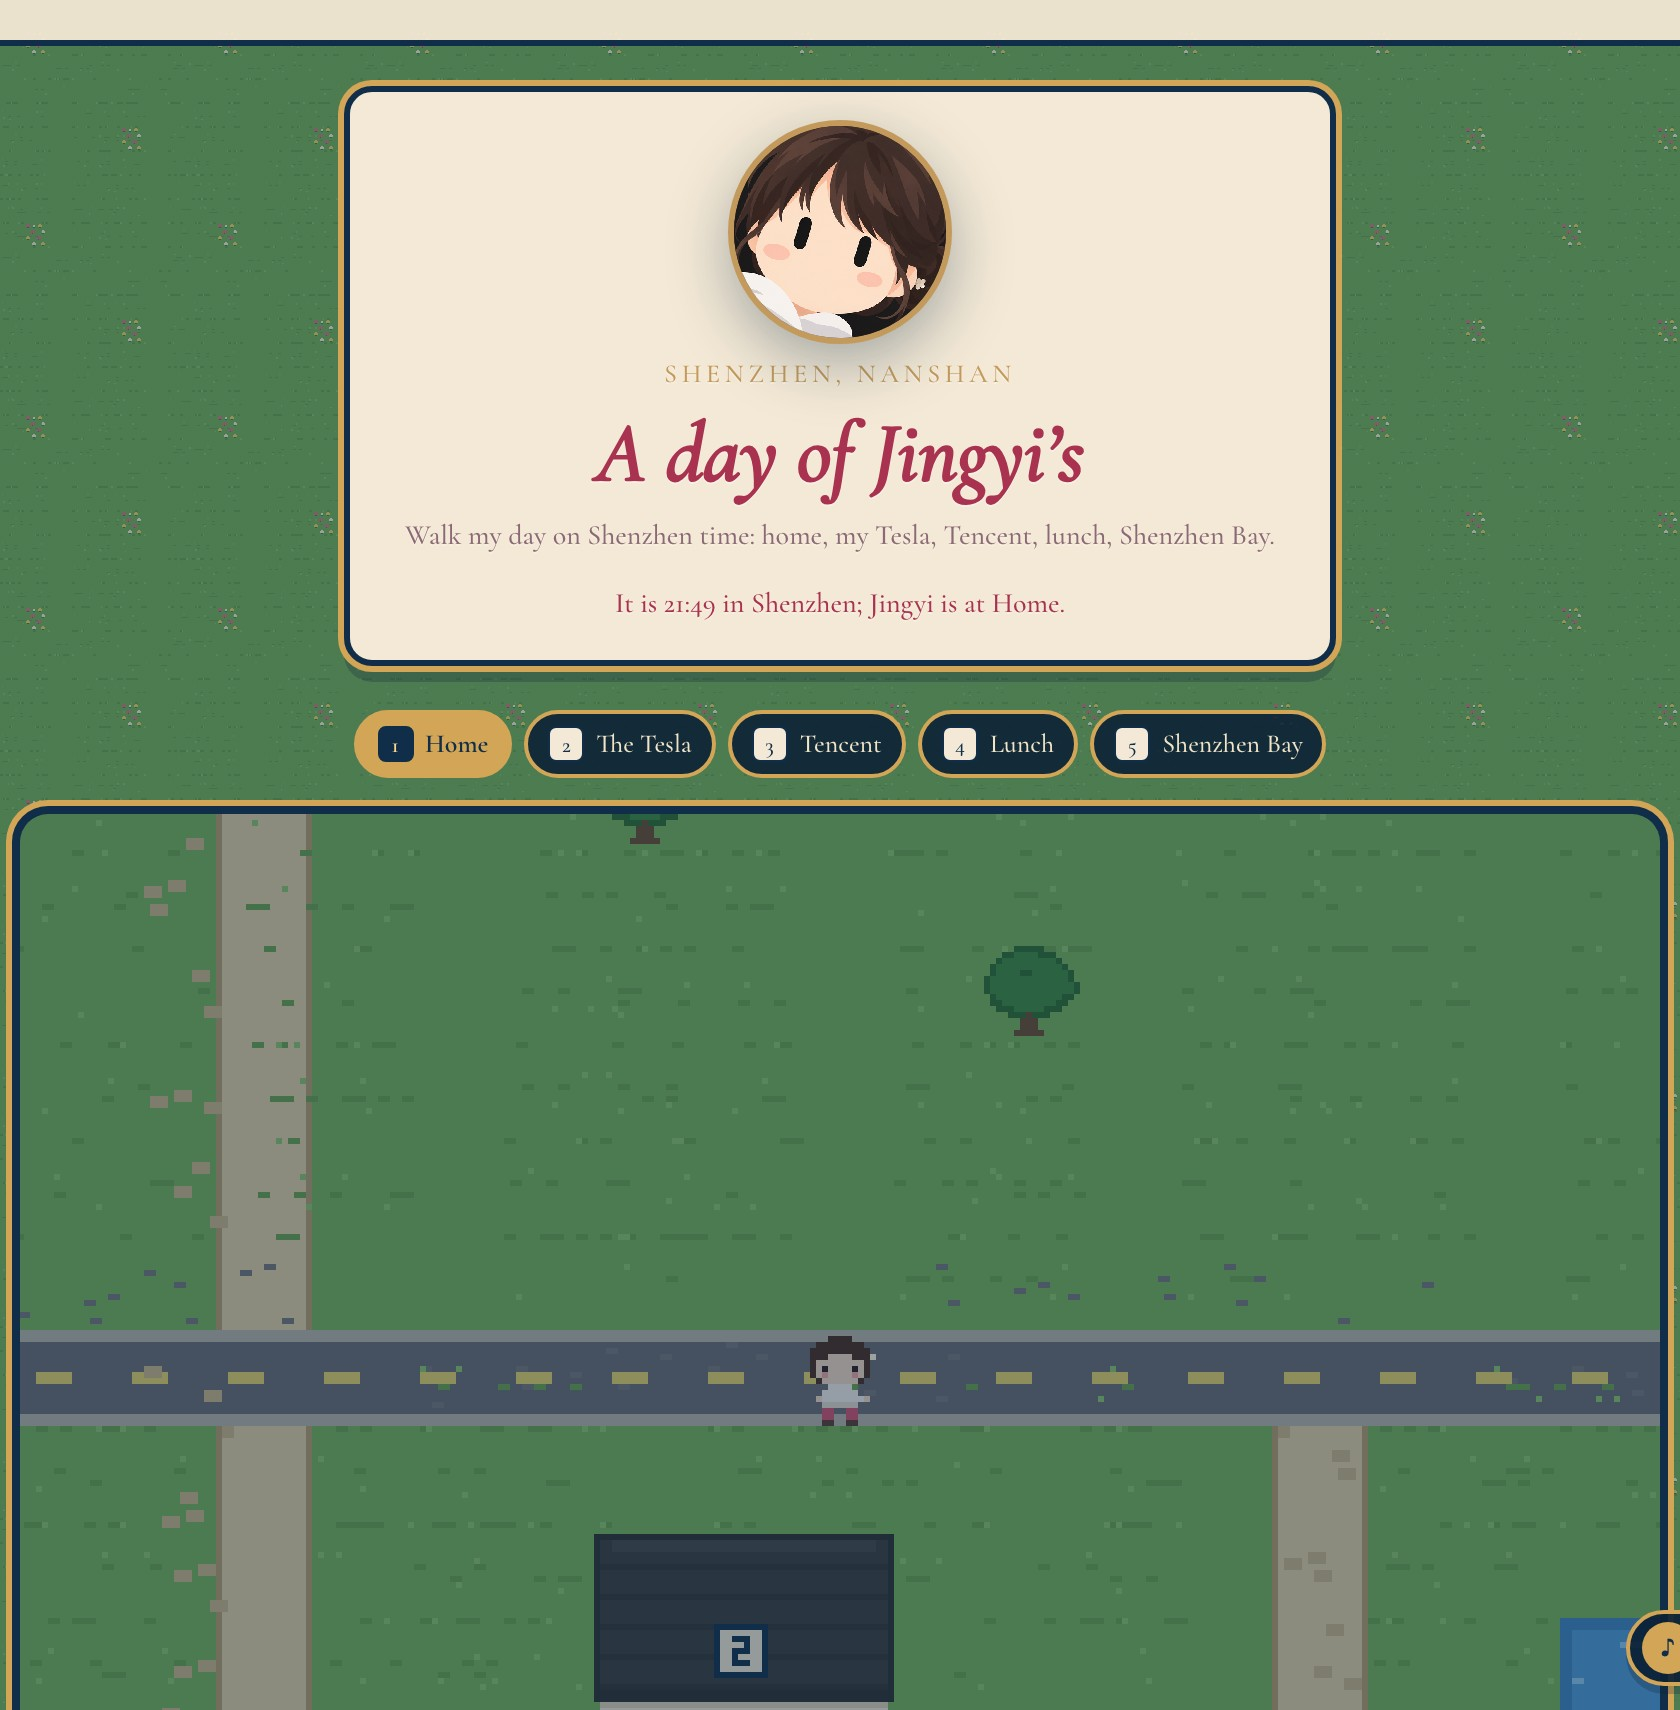
\includegraphics[width=\linewidth]{figures/page-sz.jpg}\caption{A day of Jingyi's}\end{subfigure}
  \caption{The two cities as maps. The person stands at the stop whose hours contain the current
  local time in their own city: (a) Yifan at his advisor's office at 8:49 a.m.\ in College
  Station; (b) Jingyi at home at 9:49 p.m.\ in Shenzhen, the same instant.}
  \Description{Two pixel maps with roads and buildings, each with a person card above it and a row
  of stop buttons.}
  \label{fig:days}
\end{figure}

\subsection{Prologue and finale}
Two cutscenes frame the game (Figure~\ref{fig:cutscenes}). They run in a small pixel theatre: a
$128\times80$ canvas scaled without smoothing, actors built from the town's sprite sheets, a
darkness layer with candle-like glows, particles, a synthesised score, and a caption box for words
and buttons.

\emph{The birthday prologue} plays once per player before the town opens. In College Station it is
9:47 a.m.; in Shenzhen 10:47 p.m., 73 minutes before Jingyi's birthday. Yifan, in a chef's hat,
bakes the cake against the Shenzhen clock. The player helps by whisking the batter (twelve taps),
placing ten strawberries in the same heart that the Gomoku answers make, and watching nine candles
lit (nine levels; in Chinese \zh{九} ``nine'' sounds like \zh{久} ``for a long time''). At midnight in
Shenzhen the lights go out, the door opens on the town (``In Yi Town there is no thirteen-hour
time difference''), everyone sings, the player makes a wish and blows the candles out, by
breathing into the microphone or holding a button.

\emph{The wedding} opens after the last letter, once both players have cleared the last level.
In the fountain garden at dusk, Rayford reveals why he had worn a suit all along: he is the
master of ceremonies. The groom waits under the arch, the bride walks the aisle to Mendelssohn's
\emph{Wedding March}, both say ``I do'' (aloud if the browser can listen; ``I don't'' is not
accepted), Coffee carries the rings down the aisle on a red pillow, the Meridian rings turn in
3D, and the scene ends in a kiss, bells, doves and a certificate to keep
(Figure~\ref{fig:cert}). Afterwards the town dresses the two sprites as bride and groom.

\begin{figure*}[t]
  \centering
  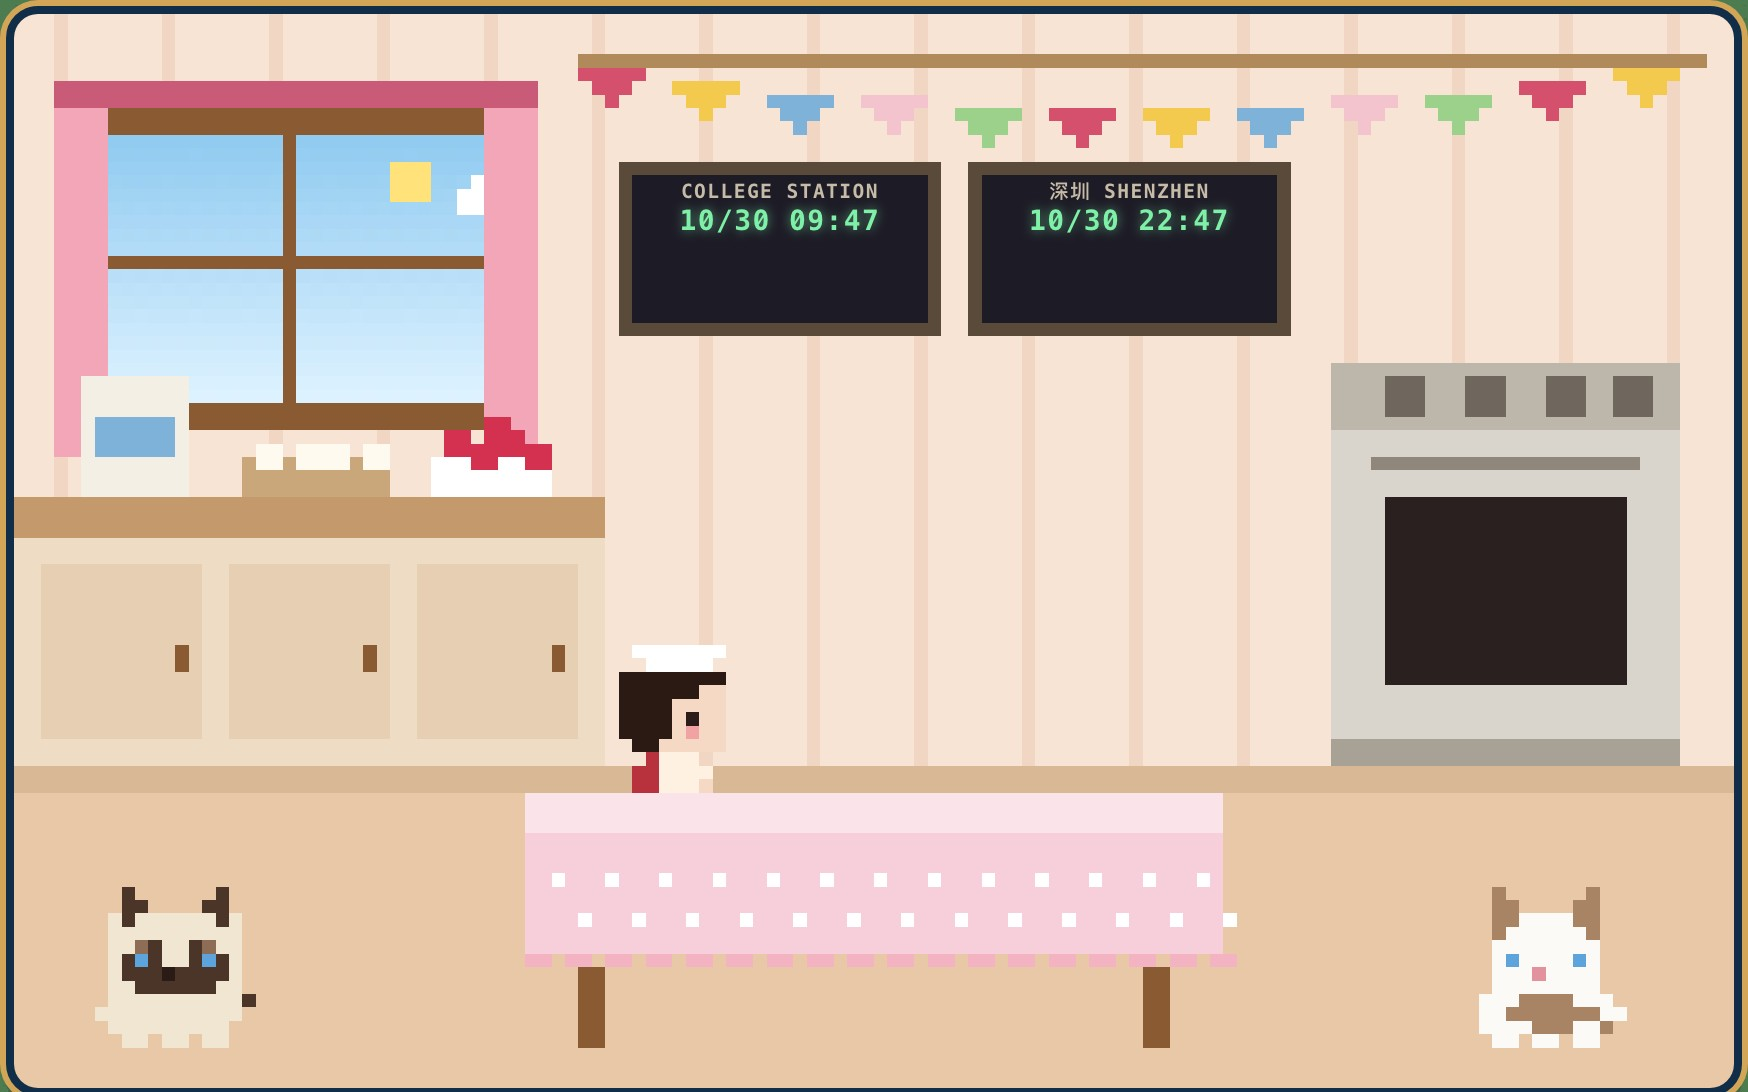
\includegraphics[width=0.245\textwidth]{figures/bday-03.jpg}\hfill
  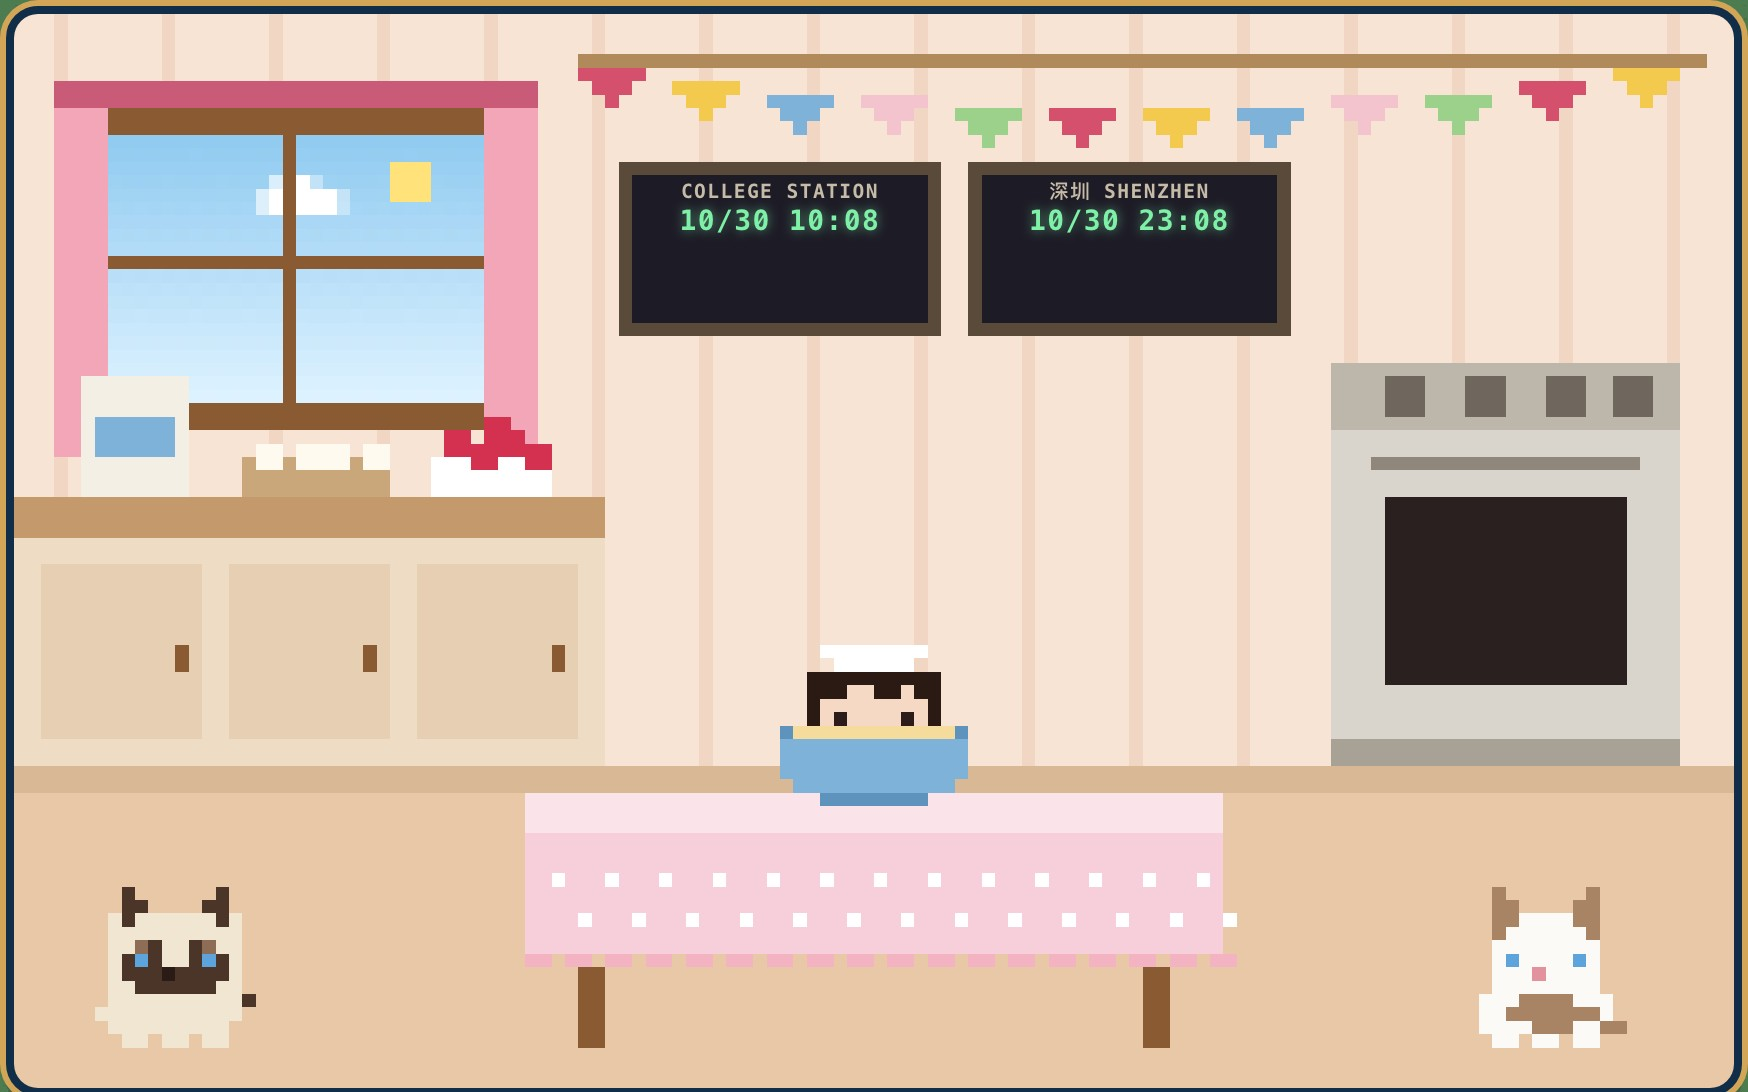
\includegraphics[width=0.245\textwidth]{figures/bday-09.jpg}\hfill
  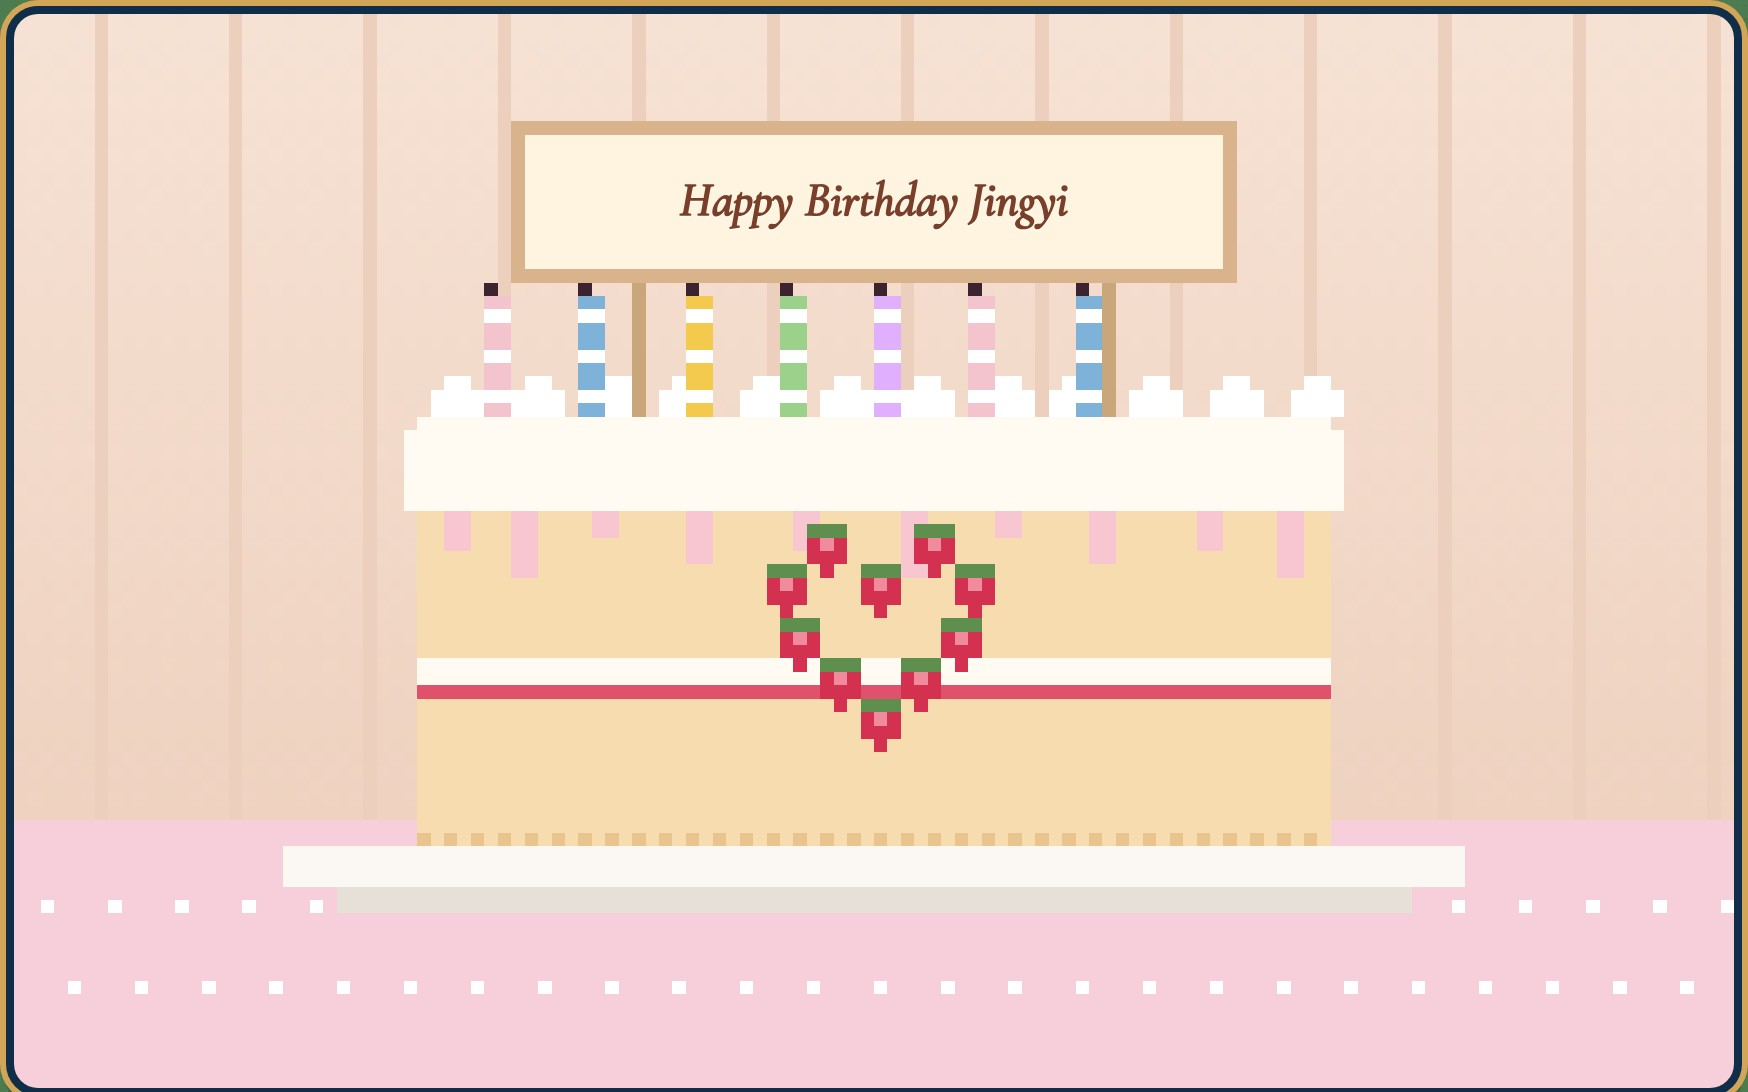
\includegraphics[width=0.245\textwidth]{figures/bday-27.jpg}\hfill
  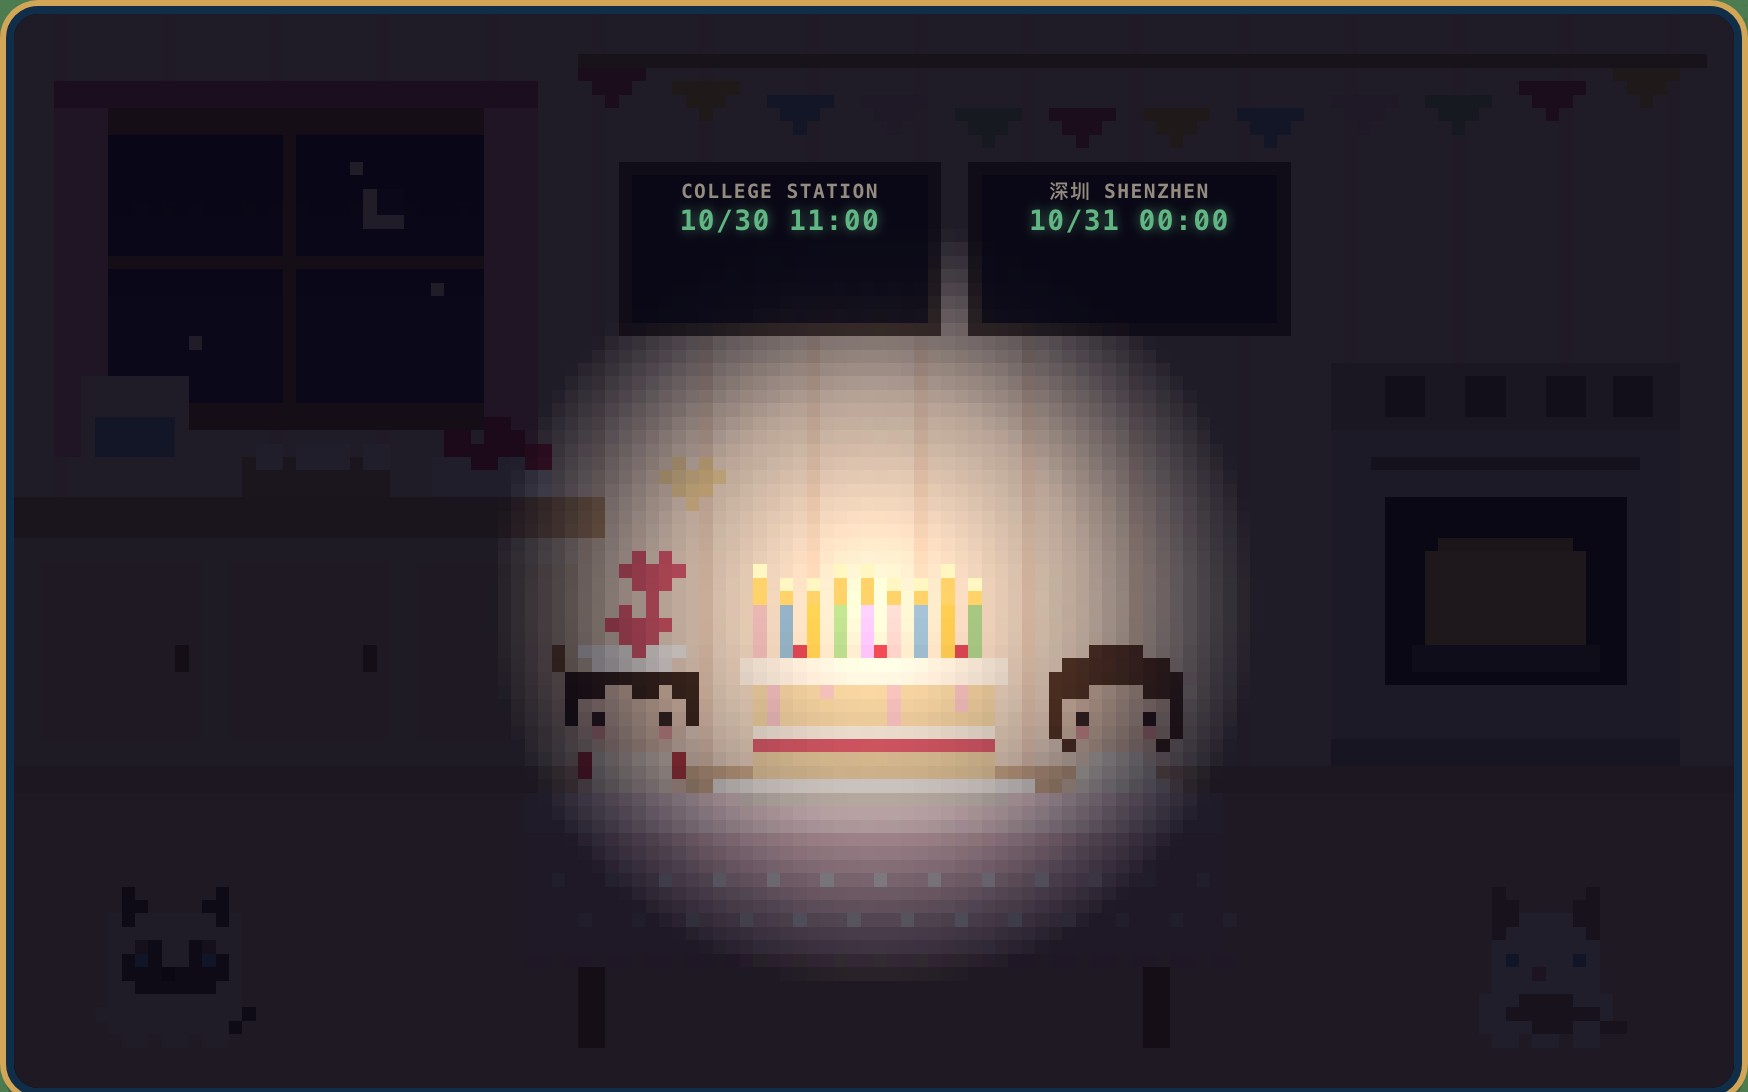
\includegraphics[width=0.245\textwidth]{figures/bday-37.jpg}\\[3pt]
  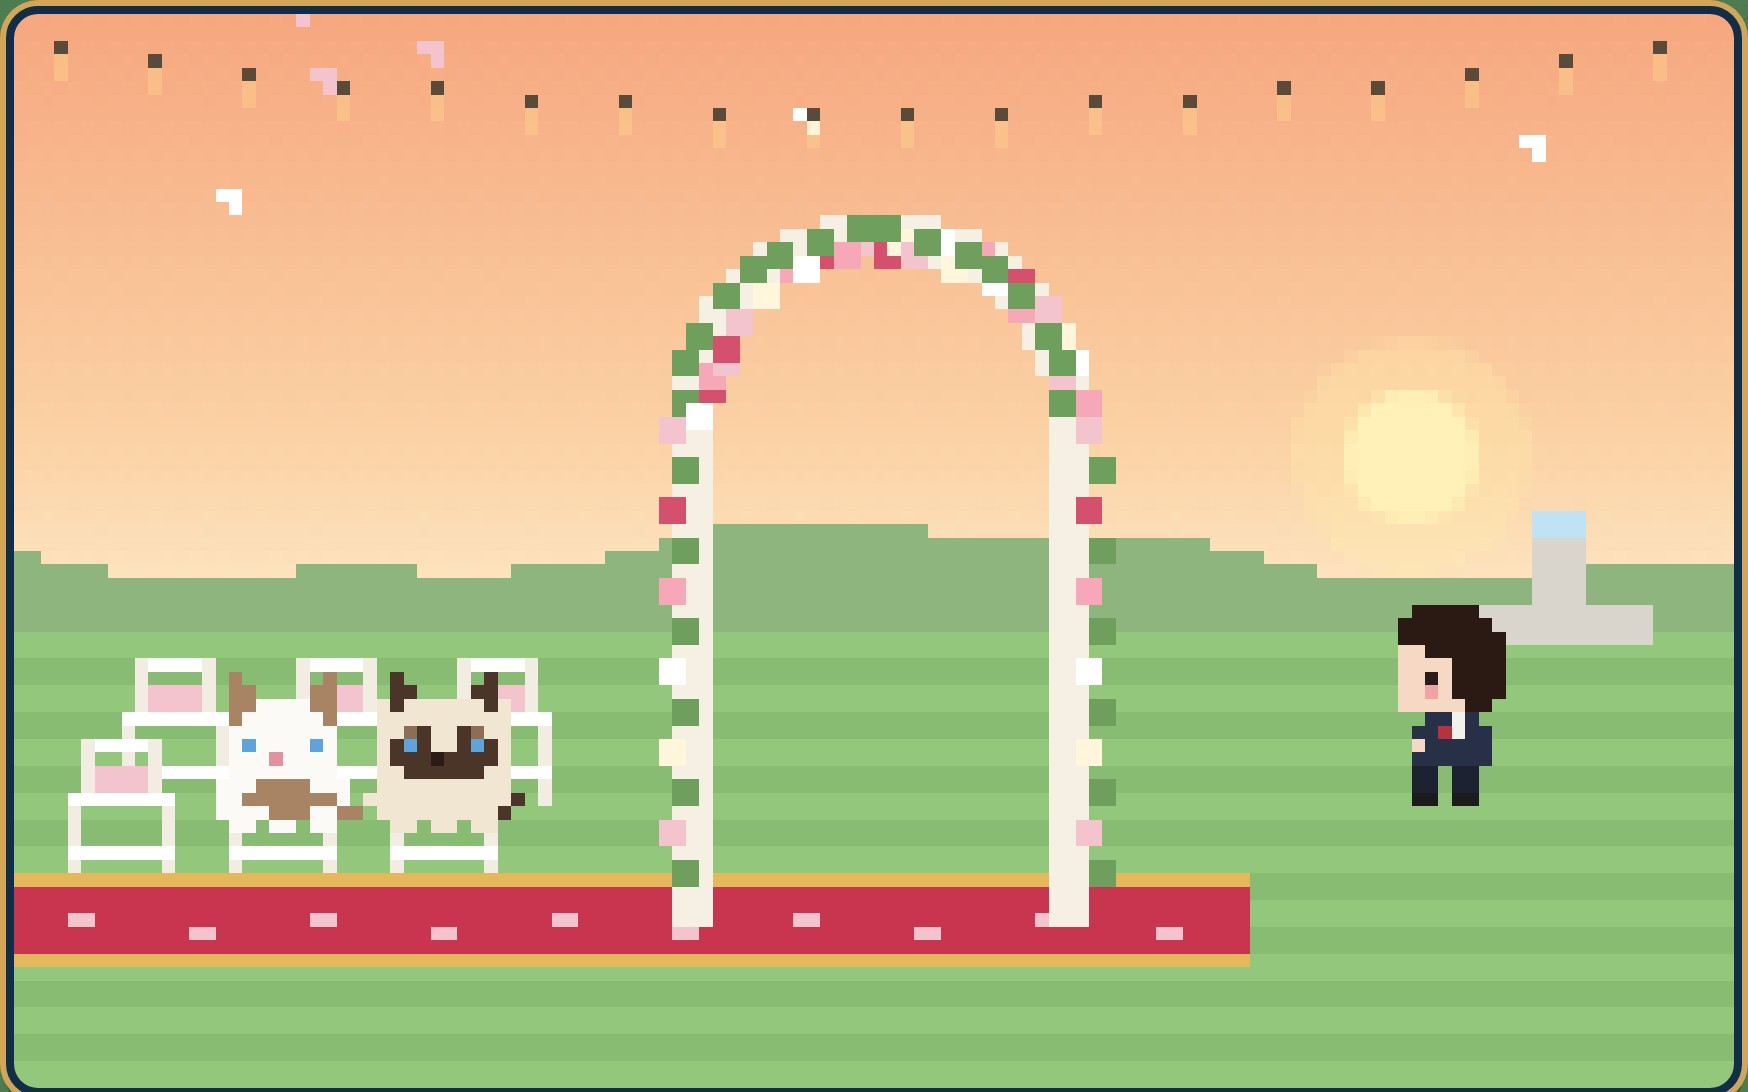
\includegraphics[width=0.245\textwidth]{figures/wed-03.jpg}\hfill
  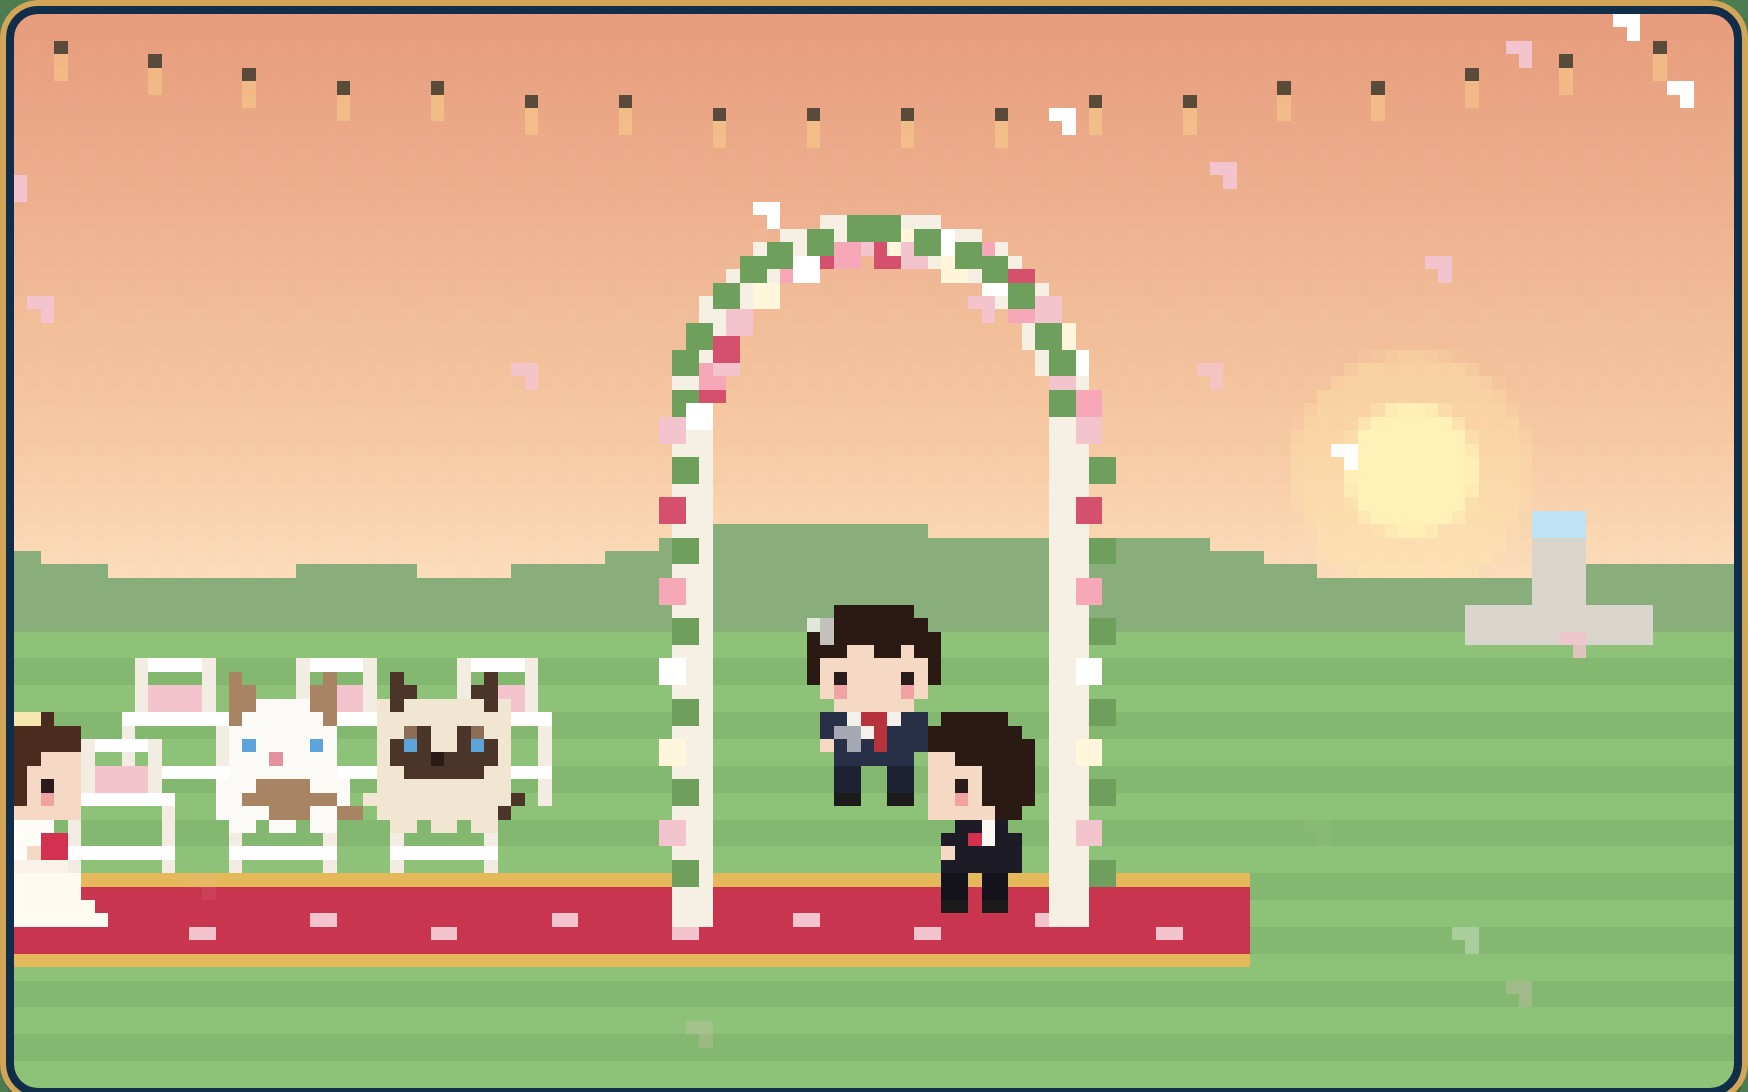
\includegraphics[width=0.245\textwidth]{figures/wed-11.jpg}\hfill
  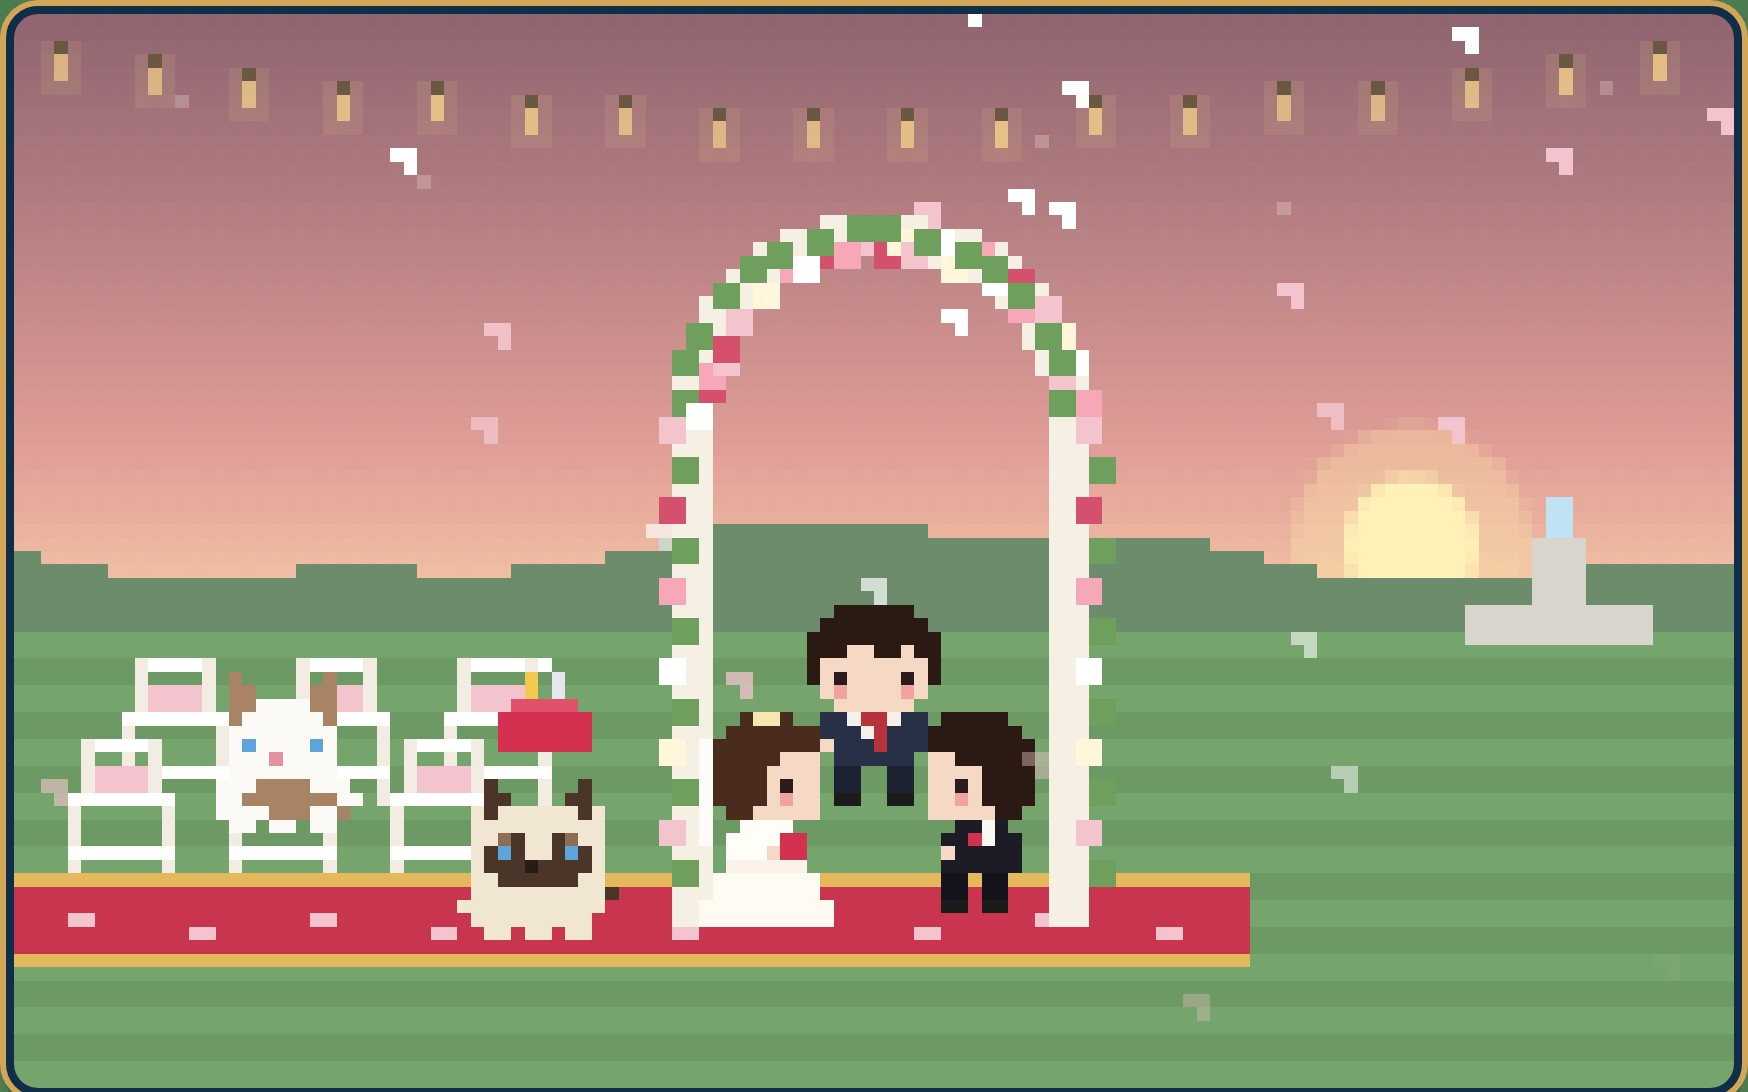
\includegraphics[width=0.245\textwidth]{figures/wed-21.jpg}\hfill
  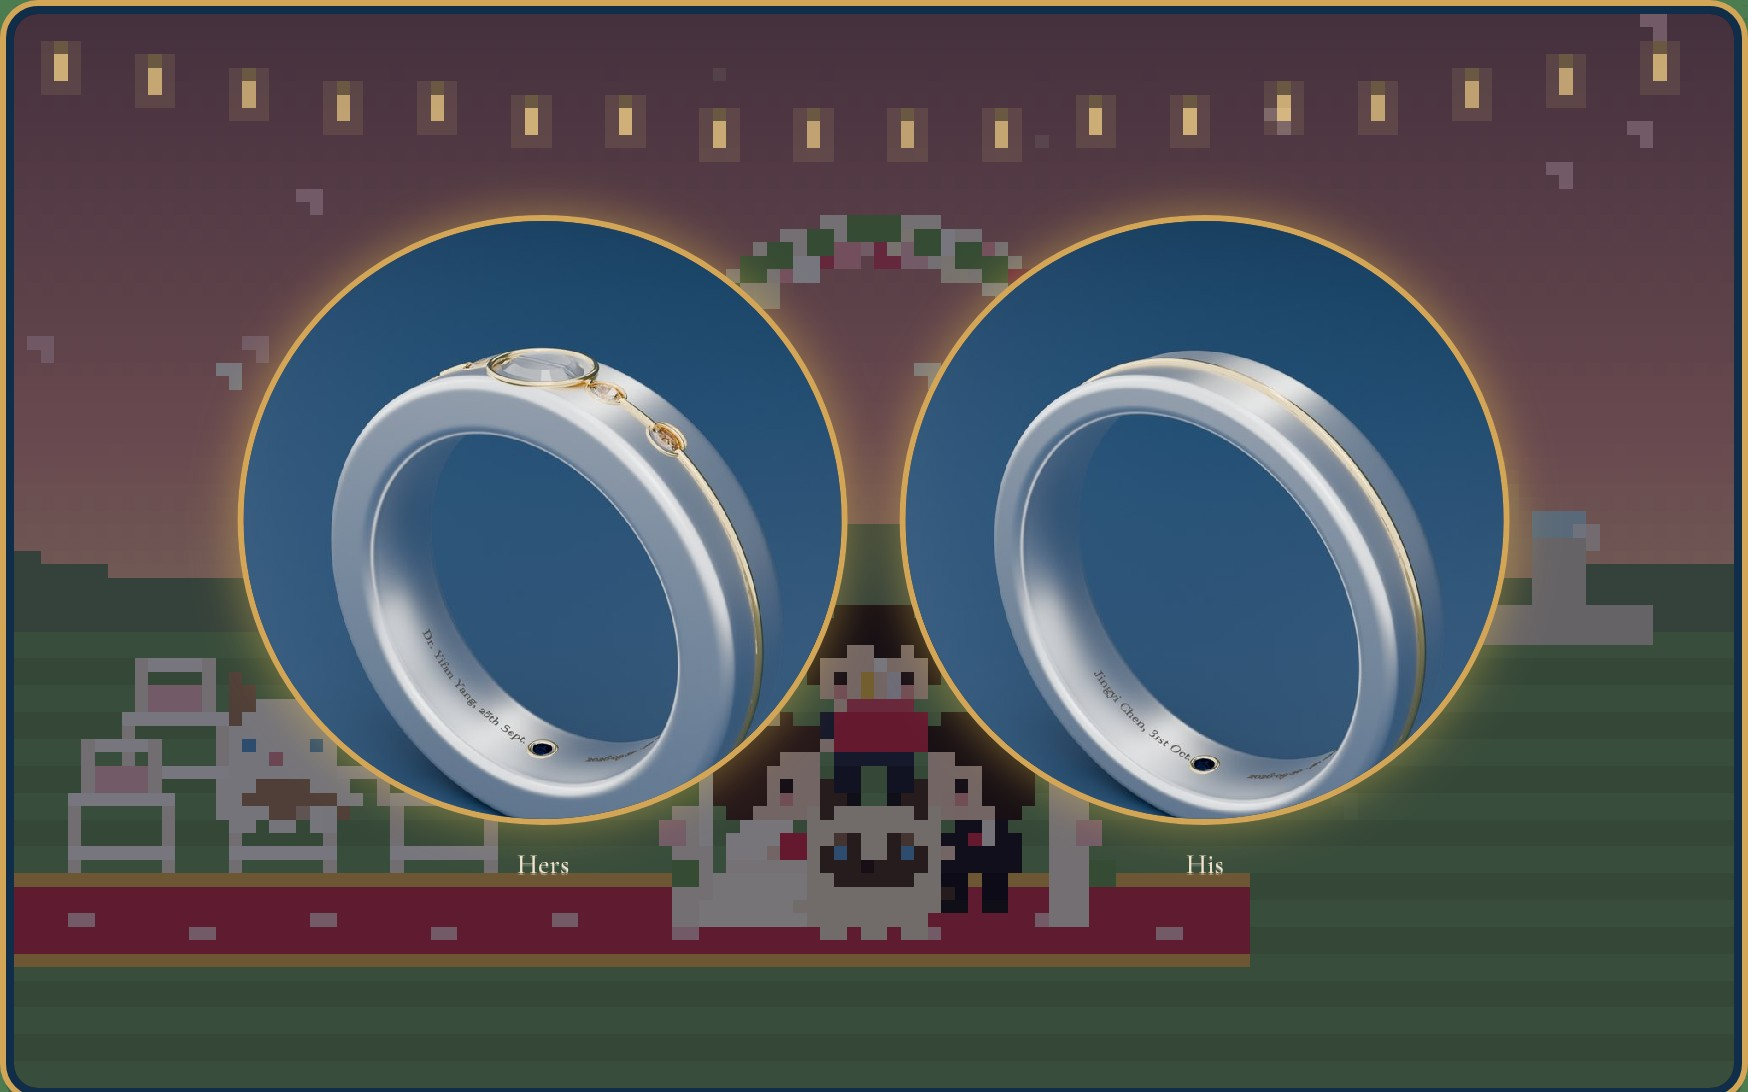
\includegraphics[width=0.245\textwidth]{figures/wed-23.jpg}
  \caption{The two cutscenes, left to right. Top, the birthday prologue: the kitchen at 9:47 a.m.\
  in College Station (10:47 p.m.\ in Shenzhen) with both clocks on the wall; whisking the batter;
  nine candles on the finished cake; singing at Shenzhen midnight with the cats. Bottom, the
  wedding: the guests take their seats; the bride walks the aisle; Coffee brings the rings; the
  Meridian rings in 3D over the ceremony.}
  \Description{Eight pixel-art frames. Top row: a pink kitchen, a chef at a table, a cake with
  candles, the same kitchen dark with candlelight. Bottom row: a garden with a flower arch at sunset,
  a couple under the arch, a cat carrying a pillow, two large 3D rings in circles.}
  \label{fig:cutscenes}
\end{figure*}

\begin{figure}[t]
  \centering
  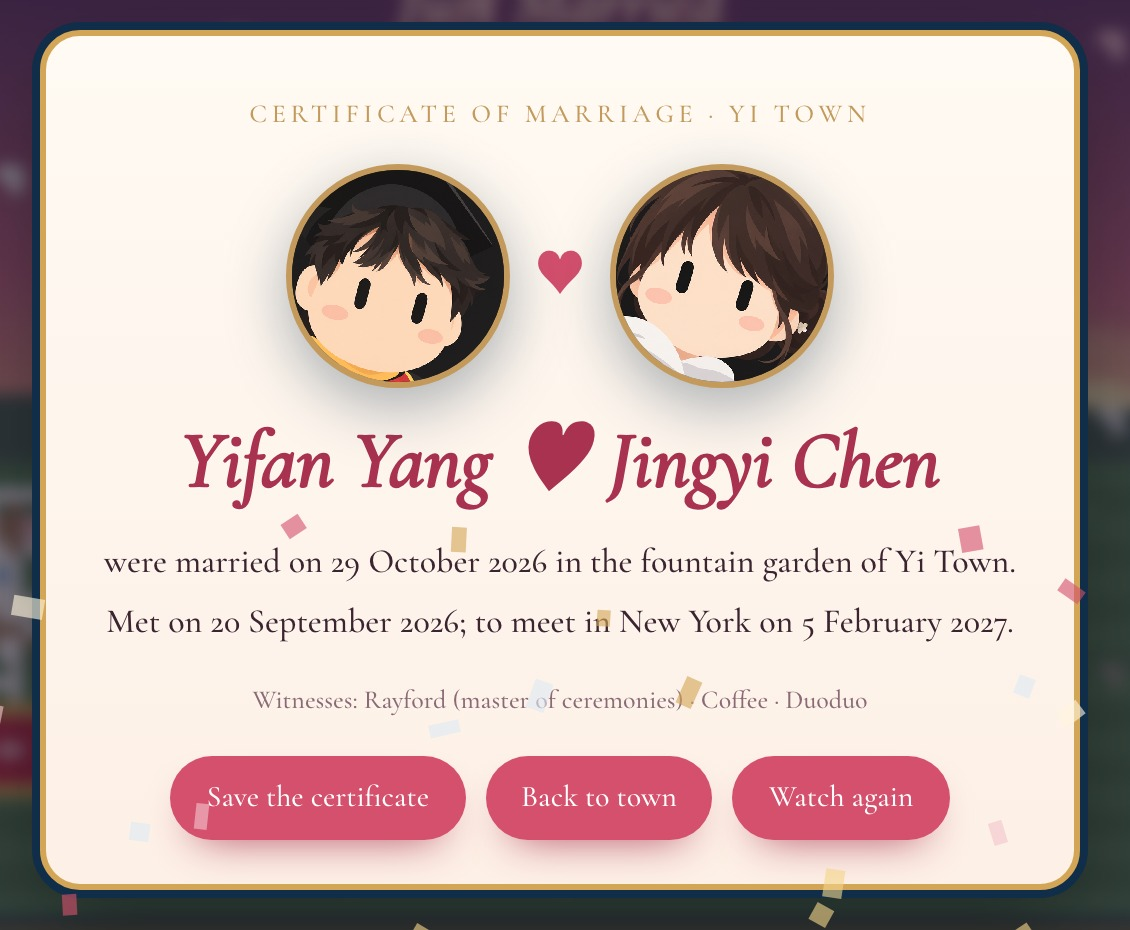
\includegraphics[width=0.78\columnwidth]{figures/wed-cert.jpg}
  \caption{The certificate at the end of the wedding, saved as an image through the phone's share
  sheet. It records the day of the ceremony, the day they met and the day they will meet.}
  \Description{A cream certificate card with two cartoon avatars and the names Yifan Yang and Jingyi Chen joined by a heart, on confetti.}
  \label{fig:cert}
\end{figure}

%% ===================================================================================
\section{System}\label{sec:system}

\subsection{Architecture}
\yt{} is a static single-page application in strict TypeScript, built with Vite and served from
GitHub Pages on the couple's own domain (Figure~\ref{fig:arch}). There is no backend. Each feature
is a folder (\code{src/features/<name>/}) with its page module, styles, data, tests and a README,
and each page is a function \code{render(root) $\Rightarrow$ cleanup} loaded lazily by a path
router, so the main bundle carries only the shell and the town. Heavy modules (Leaflet for the map,
three.js for the ring, MediaPipe for the try-on) load only inside the level that needs them. A
service worker precaches the shell, so the town installs as an app and works offline; media is
cached on first use and refreshed in the background.

\begin{figure}[t]
  \centering
  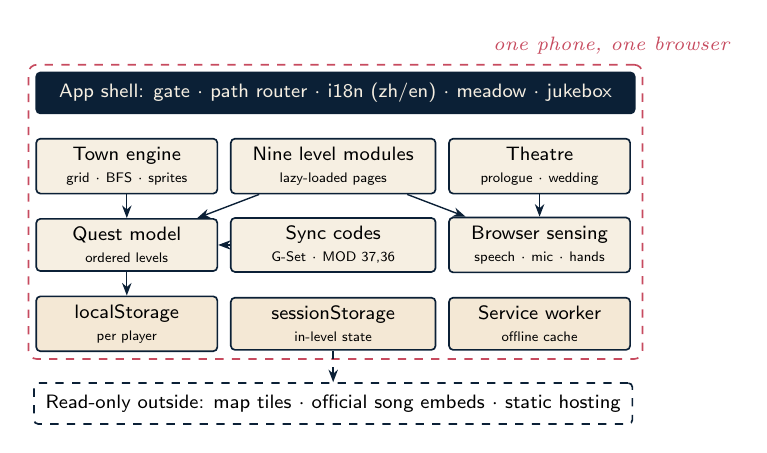
\begin{tikzpicture}[
      font=\scriptsize\sffamily,
      box/.style={draw=navy, line width=0.6pt, fill=cream, rounded corners=1.5pt, align=center, inner sep=3pt, minimum height=5.2mm},
      store/.style={box, fill=gold!25},
      ext/.style={box, dashed, fill=white},
      arr/.style={-{Stealth[length=1.6mm]}, navy, line width=0.5pt}]
    \node[box, minimum width=7.6cm, fill=navy, text=cream] (shell) {App shell: gate $\cdot$ path router $\cdot$ i18n (zh/en) $\cdot$ meadow $\cdot$ jukebox};
    \node[box, below=3mm of shell.south west, anchor=north west, minimum width=2.3cm] (town) {Town engine\\\tiny grid $\cdot$ BFS $\cdot$ sprites};
    \node[box, right=1.5mm of town, minimum width=2.6cm] (levels) {Nine level modules\\\tiny lazy-loaded pages};
    \node[box, right=1.5mm of levels, minimum width=2.3cm] (theatre) {Theatre\\\tiny prologue $\cdot$ wedding};
    \node[box, below=3mm of town, minimum width=2.3cm] (quest) {Quest model\\\tiny ordered levels};
    \node[box, right=1.5mm of quest, minimum width=2.6cm] (sync) {Sync codes\\\tiny G-Set $\cdot$ MOD 37,36};
    \node[box, right=1.5mm of sync, minimum width=2.3cm] (sense) {Browser sensing\\\tiny speech $\cdot$ mic $\cdot$ hands};
    \node[store, below=3mm of quest, minimum width=2.3cm] (ls) {localStorage\\\tiny per player};
    \node[store, right=1.5mm of ls, minimum width=2.6cm] (ss) {sessionStorage\\\tiny in-level state};
    \node[store, right=1.5mm of ss, minimum width=2.3cm] (sw) {Service worker\\\tiny offline cache};
    \node[ext, below=4mm of ss, minimum width=7.6cm] (ext) {Read-only outside: map tiles $\cdot$ official song embeds $\cdot$ static hosting};
    \node[draw=rose, dashed, rounded corners=3pt, line width=0.6pt, fit=(shell)(ls)(sw), inner sep=2.5pt,
          label={[rose, font=\scriptsize\itshape]above right:one phone, one browser}] {};
    \draw[arr] (town) -- (quest); \draw[arr] (levels) -- (quest); \draw[arr] (levels) -- (sense);
    \draw[arr] (theatre) -- (sense); \draw[arr] (quest) -- (ls); \draw[arr] (sync) -- (quest);
    \draw[arr, dashed] (ss.south) -- (ext.north);
  \end{tikzpicture}
  \caption{Architecture. Everything that holds the couple's data stays inside the browser (dashed
  red); the outside world is read only, and only for map tiles, song embeds and the static files
  themselves. A second phone joins through a code, not a server.}
  \Description{A block diagram: an app shell above three modules, which depend on a quest model,
  sync codes and browser sensing, which sit above three storage layers, all inside a dashed boundary
  labelled one phone, one browser; a dashed box below for read-only external resources.}
  \label{fig:arch}
\end{figure}

\subsection{The quest model}
Let $L = (\ell_1,\dots,\ell_9)$ be the ordered level registry and $C_p \subseteq L$ the set of
levels player $p$ has cleared on a device. A level is unlocked iff it is first or its predecessor
is cleared:
\begin{equation}
  \mathrm{unlocked}_p(\ell_i) \iff i = 1 \;\lor\; \ell_{i-1} \in C_p .
\end{equation}
Clearing adds to $C_p$ and nothing ever removes from it, except an explicit reset. The router
enforces the lock, and a second guard requires that a level be entered through its door: walking
onto the door sets a one-shot token in \code{sessionStorage}, and a level route without the token
redirects to the town. Level numbers are derived from the registry, so inserting a level (the
Poems level was inserted before the last one during development) renumbers every house, sign and
string at once; a test fails until the new house has a door that the town's path search can reach.

\subsection{Progress without a server}
Each phone holds its own $C_p$. Because $C_p$ only grows, it is a grow-only set (G-Set), the
simplest state-based CRDT~\cite{shapiro2011crdt}: the merge of two replicas is their union,
\begin{equation}
  C_p \sqcup C'_p = C_p \cup C'_p ,
\end{equation}
which is commutative, associative and idempotent. Two phones that exchange codes in any order, any
number of times, therefore converge, and importing an old code can never take progress away. The
only channel needed is one the couple already use every day: a chat message.

\paragraph{Progress codes.} A code encodes one player and a bitmask of cleared levels,
$m = \sum_{\ell_i \in C_p} 2^{\,i-1}$, written in base 36 after a player letter (\code{J} or
\code{Y}) and followed by one check character. With nine levels $m \le 511 = \mathrm{E7}_{36}$, so a
code is at most four characters: \code{JVA} says that Jingyi has cleared $m = 31$, the first five
levels (Table~\ref{tab:codes}). The check character follows the hybrid system ISO~7064
MOD~37,36~\cite{iso7064}. Writing $a_j \in \{0,\dots,35\}$ for the value of the $j$-th body
character and starting from $p_0 = 36$,
\begin{equation}
  s_j = \big((p_{j-1} + a_j) \bmod 36\big) \text{ or } 36 \text{ if } 0, \qquad
  p_j = 2 s_j \bmod 37 ,
\end{equation}
and the check character is the symbol of value $(37 - p_n) \bmod 36$. We checked the scheme exhaustively over all
1{,}024 valid codes. It rejects every one of the codes' single-character substitutions. Of the
2{,}943 transpositions of two different adjacent characters, it rejects all but five. One of
those (\code{JI0}$\to$\code{IJ0}) is still refused because \code{I} is not a player letter. The
other four all swap a \code{0} and a \code{1} inside the mask (\code{J801}$\leftrightarrow$\code{J810},
\code{YE01}$\leftrightarrow$\code{YE10}): the rule above maps a running sum of 0 to 36, so a zero
digit and its neighbour can trade places unseen. Substitutions and adjacent swaps are the two
mistakes people make when copying a code from a chat, and in practice a swapped code that passes
is still a valid code for the same player, so the union merge can at worst add levels
that were not cleared. An earlier version used a plain weighted sum,
which let some one-character typos through; it was replaced during a review pass, invalidating older
codes. A code can also travel inside a link (\code{/sync?c=JVA}), which imports it when opened.

\begin{table}[t]
  \caption{Example progress codes: player letter, base-36 mask and the check character of Eq.~3.}
  \label{tab:codes}
  \small
  \begin{tabular}{@{}lrll@{}}
    \toprule
    Cleared & Mask $m$ & Base 36 & Code \\
    \midrule
    Jingyi, levels 1--5 & 31 & \code{V} & \code{JVA} \\
    Jingyi, all nine & 511 & \code{E7} & \code{JE7Z} \\
    Yifan, all nine & 511 & \code{E7} & \code{YE7O} \\
    Yifan, none & 0 & \code{0} & \code{Y0C} \\
    \bottomrule
  \end{tabular}

\end{table}

\paragraph{Three layers of storage.} Cleared levels live in \code{localStorage} under a key per
player; half-finished state inside a level (the Gomoku position reached, the stars joined so far)
lives in \code{sessionStorage}, so a reload or a language switch inside a level does not restart it,
and it is dropped when the level is cleared; and a service worker keeps the site itself. When the
browser blocks storage, an in-memory store keeps progress for the visit.

\subsection{The town engine}
The town is a grid of characters (\code{.}\ grass, \code{\#} path, \code{\textasciitilde}\ water,
\code{T} tree, \code{O} fountain, and so on). Movement is one tile per 190\,ms with an ease-out
interpolation; the pure functions \code{step} and \code{faced} decide movement and facing and are
unit-tested, while a class wires them to a canvas and one animation loop. A tap on the map runs a
breadth-first search over walkable tiles and queues the resulting steps. The camera follows the
player. The same engine takes any map, so the two cities reuse it with their own grids, roads and a
basketball court.

\paragraph{Art as text (\dc{5}).} A sprite is an array of strings, one character per pixel, and
a palette that maps characters to colours. A figure is a $12\times12$ body per facing over four
rows of legs shared between facings, so a walk cycle is the same two leg frames under different
bodies, and the side view is mirrored. Tiles (grass with flowers, paths that join their neighbours,
roofs in each level's colour, lit windows) are painted procedurally. The README banner, the favicon
and the app icons are generated from the same strings by scripts, so a new outfit appears
everywhere at once.

\paragraph{Daylight by city.} Let $h_p$ be the current hour in player $p$'s time zone
(\code{Asia/Shanghai} or \code{America/Chicago}). The phase is dawn for $h_p \in [6,7)$, day for
$[7,17)$, dusk for $[17,19)$ and night otherwise; dawn, dusk and night each lay a coloured wash over
the map (night: navy at 42\% opacity) and light the windows. In the two cities the person's
position is $\mathrm{stopAt}(h) = $ the first stop whose hour windows contain $h \bmod 24$.

\subsection{Sensing in the browser}\label{sec:sensing}
Three levels listen or look, and none sends a frame or a sample anywhere.

\emph{Voice.} The vow and the wedding's ``I do'' use the Web Speech API~\cite{w3c2023speech} in
Mandarin. All recognition alternatives are joined and normalised to Han characters and Latin
letters; a vow counts when it contains \zh{我爱你}, \zh{我愿意} and any accepted spelling of the
partner's name.

\emph{Breath.} Blowing out the candles reads the microphone with echo cancellation, noise
suppression and gain control off, computes the root-mean-square loudness of each 1{,}024-sample
frame, smooths it ($s \leftarrow 0.6s + 0.4\min(1, 5\,\mathrm{rms})$), and blows when $s > 0.32$.
A breath on a phone microphone is a loud broadband rush, so this simple rule is enough.

\emph{Hands.} The try-on runs MediaPipe's hand landmarker~\cite{lugaresi2019mediapipe,zhang2020hands}
on the camera stream. The ring sits on the ring finger's proximal phalanx, 38\% of the way from
landmark 13 (the knuckle) to landmark 14; its axis follows the finger, and its ``up'' is the back of
the hand, from the palm normal and the reported handedness. Scale comes from anatomy: the mean
spacing of the middle, ring and little knuckles, about 19.5\,mm in adults, serves as the ruler, so
\begin{equation}
  \text{px/mm} = \tfrac{1}{2}\,\big(\lVert k_9 - k_{13}\rVert + \lVert k_{13} - k_{17}\rVert\big) \,/\, 19.5 ,
\end{equation}
and the ring's real millimetre dimensions map to the screen. Position, rotation and scale are
smoothed (factor 0.45 per frame). The shutter composes the photo with a caption, and a second card
puts both players' try-on photos side by side.

\subsection{Keeping a secret with a test (\dc{6})}
The ring is the surprise at the end, and an interface that hints at it spoils it. Rayford, the
town, the progress page and the cats all speak before the ring is reached, and their lines were
written and rewritten over days. Rather than rely on vigilance, a unit test scans every key in
the bilingual dictionary, except the keys shown only after the ring, and fails if any contains
\zh{戒} (ring) in Chinese, \emph{ring} as a word in English, or any word for wedding, marriage,
proposal, bride or groom in either language. One exception is listed by name: Jingyi's own joke on
the Shenzhen Bay stop, which is about a flat, not a ring. The test turns a promise into a property
of the build.

\subsection{Implementation and verification}
Table~\ref{tab:metrics} summarises the code base. The main bundle is 114\,kB (43\,kB compressed);
the three heaviest chunks (the ring viewer with three.js, the map with Leaflet, the try-on) load
only in their levels. Continuous integration runs the 153 unit tests and the strict type check on
every push and deploys while publishing is switched on. Beyond unit tests, each release was checked
with a scripted play-through of all nine levels in a headless browser and a sweep of every page at
320, 390 and 1{,}280 pixels wide in both languages. Some features cannot be verified headless and
were tested on real phones: speech, the breath detector, the camera try-on and the share sheet.

\begin{table}[t]
  \caption{Implementation summary (version 1.17.0, 28 October 2026).}
  \label{tab:metrics}
  \small
  \begin{tabular}{@{}lr@{}}
    \toprule
    Measure & Value \\
    \midrule
    TypeScript source, excluding tests (lines) & 8{,}414 \\
    CSS (lines) & 1{,}080 \\
    Bilingual dictionary (lines) & 791 \\
    Test files / unit tests & 36 / 153 \\
    Commits / versions (24--28 Oct.\ 2026) & 109 / 28 \\
    Main bundle (min.\ / gzip) & 114\,kB / 43\,kB \\
    Precached shell (service worker) & 44 files, 302\,KiB \\
    Feature folders & 24 \\
    Runtime dependencies & 3 (Leaflet, three.js, MediaPipe) \\
    Servers, accounts, analytics & 0 \\
    \bottomrule
  \end{tabular}
\end{table}

%% ===================================================================================
\section{Reflections from the Design Log}\label{sec:log}

Several changes the owner made to his own system show where a reasonable default failed for these
two people.

\paragraph{From Pictionary to songs.} An early level was Pictionary, after the couple's first
evening of games, played on one device by turns. The owner replaced it with \emph{Our Songs}. Our
reading of the change is that a drawing game played by turns assumes two people at one screen,
which this couple never are, whereas a song can be recognised alone and still brings the other
person's music with it.

\paragraph{From reveal to photograph.} The ring level was at first cleared by watching the reveal.
The owner changed the rule so that only the try-on photo clears it: the level asks for an act, not
for attention, and leaves an image to send.

\paragraph{Getting the person right.} Generated defaults guessed that Yifan takes the bus and that
Jingyi takes the metro, and named the baker in the prologue after Yifan's nickname. Each was
corrected: Yifan drives; Jingyi drives a Tesla; the baker is Yifan himself. For an audience of one,
a plausible guess about her life reads as not knowing her.

\paragraph{One question at the door.} The gate's placeholder text once spelled out the answer.
A review pass removed it. The gate protects little (Section~\ref{sec:privacy}), but a door that
answers its own question is no longer a question only the two of them can answer.

%% ===================================================================================
\section{Discussion}\label{sec:discussion}

\subsection{Memory as mechanics}
Hassenzahl et al.\ found \emph{memories} to be one strategy among six~\cite{hassenzahl2012love}; in
\yt{} it is the grammar of the whole system. The interesting design work was not choosing which
memories to include but finding the \emph{rule} each memory implies. A first game on a whiteboard
implies Gomoku, but ``win-in-one'' implies something more: that each step is a small discovery, and
that ten discoveries can add up to a shape. The heart then recurs: as gold stones on the board, as
strawberries on the cake, as the outline the player follows. Repeated motifs let a small system feel
authored rather than assembled.

\subsection{Privacy as intimacy, not security}\label{sec:privacy}
The gate is not security. Its answers are dates, and a determined attacker could enumerate them in
moments; the SHA-256 hash only keeps the answer from being read in the source. Its purpose is
social: the site asks a question only the two of them can answer, and that question is itself a
small ritual of recognition. Likewise, keeping all progress on the device (\dc{3}) is less about
threat models than about where the couple's things live. A voice note in a mailbox in a town on her
phone is a different object from the same audio on a server. Local-first software~\cite{kleppmann2019localfirst}
usually argues for ownership and longevity; here the argument is closeness.

\subsection{Thirteen hours}
Asynchrony is often treated as a problem to be bridged with presence. \yt{} treats it as material.
Each player's town is lit by their own clock, so the two never see the same sky; the partner by the
fountain is a message left, not a presence; and the birthday prologue is staged precisely on the
gap, a morning in Texas that is the last hour before midnight in Shenzhen. The prologue's line ``In
Yi Town there is no thirteen-hour time difference'' works because everything before it has shown the
difference. This echoes slow technology's interest in time as a design
material~\cite{hallnas2001slow,odom2012technology}.

\subsection{Secrecy as a design material}
Surprise is fragile in software: any string, any loading screen, any helpful guide can leak it. We
found it useful to treat the surprise as an invariant and to test it, as one tests that a list is
sorted. The secrecy test also shaped the writing: Rayford had to explain why he wears a suit without
saying why, and the answer is paid off only in the wedding. Ambiguity, here, was not a
resource~\cite{gaver2003ambiguity} so much as a promise held open.

\subsection{Two languages, one voice}
Writing every string twice, by the same author, made the two languages talk to each other. Puns
cross the boundary: the title \zh{仪见钟情} replaces the \zh{一} of \zh{一见钟情} (love at first
sight) with the \zh{仪} of Jingyi's name, a pun that cannot be translated, so the English site names
it and explains it. Nine candles mean ``for a long time'' only in Chinese, and the English caption
says so. Parity (\dc{4}) meant that neither reader is given the translated version.

\subsection{Building with an AI pair programmer}
\yt{} was built in five days by one person working with an AI coding assistant. The assistant
wrote most of the code from the owner's descriptions; the owner chose every memory, line, rule and
correction. Two practices kept the result personal rather than generic: the owner corrected
defaults about their lives as soon as he saw them (Section~\ref{sec:log}), and invariants that mattered to him
were written as tests rather than as instructions, which an assistant can forget.

\subsection{Limitations and future work}
\yt{} is a sample of two, and its first real play is Jingyi's birthday; this paper describes the
artefact and its making, not her experience, which we will report after it has happened, in her
own words. The two players cannot yet play at the same time over a network; the songs depend on
official embeds that may not play in every region; the quizzes can be brute-forced by guessing; and
several features (speech, breath, camera) depend on browser support that varies across phones. The
owner's next steps are to rewrite the two letters in his own words, add voice notes, and build
a second map, a long road from Shenzhen to College Station.

%% ===================================================================================
\section{Conclusion}
We described \yt{}, a game for two people who live thirteen hours apart, built by one of them out
of what they share. Its architecture is deliberately small: a grid, some strings that are pictures,
a grow-only set, a four-character code, a test that keeps a secret. Its content is deliberately
large: a vow, six places, a tattoo, forty days, a heart of stones, six songs, two constellations,
five poems, a ring, a cake and a wedding. For an audience of exactly one other person, technical
choices and emotional ones turned out to be the same choices, and we hope the commitments listed
here are useful to others who build for the person on the other side of the ocean.

\begin{acks}
To Coffee and Duoduo, who guard the doors. The street-view photographs on the Love Map are from
Wikimedia Commons and credited in the game; the \emph{Wedding March} is a public-domain recording
from the European Archive. The code was written with Claude Code, an AI coding assistant; every
memory, line and decision is ours. This paper, too, was drafted with the assistant from the
repository and checked by the authors.
\end{acks}

\balance
\bibliographystyle{ACM-Reference-Format}
\bibliography{references}

\end{document}
